\chapter{多元函数积分}
\label{chap:multivariate-integration}

累计范围由区间变成平面区域、空间曲线或曲面时，需要分别确定每个小块的体积、长度或面积；计算做功和通量时，还须记录行进方向或法向。本章建立这些积分并比较它们所累计的对象，再研究内部变化和边界累计之间的关系。

区域积分承接一元Riemann积分，先建立Jordan区域上的分割和，再讨论累次积分、换元和参数积分。路径积分与曲面积分分别使用弧长和面积，也讨论带方向的功与通量。最后，Green、Gauss和Stokes公式把区域或曲面内部的导数累计与其边界上的累计联系起来；使用每个公式时都要核对光滑性、可积性和方向条件。

\section{区域积分的定义与性质}
\label{sec:multivariable-region-integration}

一块不均匀的金属薄片占据平面区域$D$，在点$(x,y)$附近每单位面积的质量为$\rho(x,y)$。
把$D$切成许多小块，每块的质量约等于块内某一点的密度乘这块的面积；把所有小块的质量相加，就得到总质量的近似值，小块切得越细，近似越准确。
空间物体的质量、带电体的总电荷也按同样方式累计，只是面积换成体积，面密度换成体密度或电荷密度。
这类问题中的被积函数都是多元标量函数$f:D\subseteq\mathbb R^d\to\mathbb R$：输入是一个位置的$d$个坐标，输出是该位置上一个待累计的数。

同一个积分还有两种常用读法。
若$f\geq0$定义在平面区域$D$上，积分等于以$D$为底、以$f$的图像为顶的立体的体积，这是一元积分“曲线下方面积”在高一维的对应。
当$D$的面积有限且非零时，把积分除以面积，所得的数是$f$在$D$上的平均值，例如一个地区的平均降雨量或一块薄板的平均温度。

本章从有界区域上的Riemann积分出发。先定义分割与累计，再用截面、坐标变换和参数求导组织计算。一般可测函数与积分极限定理在\BookChapterRef{chap:integration}{第~\ref{chap:integration}章}中建立，这里不以它们为前提。

\subsection{盒体积与Jordan区域}

闭坐标盒$Q=\prod_{j=1}^d[a_j,b_j]$的体积定义为$\operatorname{vol}(Q)=\prod_j(b_j-a_j)$。某条边长度为零时体积为零。

沿任意坐标把盒切成有限块，切开的边长相加仍等于原边长，因此小盒体积之和等于原体积；对有限网格反复应用便得到有限可加性，公共的盒边界不重复贡献体积。

对有界集合$D\subset\mathbb R^d$，用有限个内部互不相交的盒从内侧和外侧逼近$D$。若每个$\varepsilon>0$都能选取这样的内、外有限盒并，使外侧总体积与内侧总体积之差小于$\varepsilon$，称$D$为Jordan可测集合。这个共同逼近的极限称为$D$的Jordan体积，记为$|D|$。

体积不依赖所选网格：任取一组内逼近和另一组外逼近，前者体积不超过后者；当两侧差距可任意小时，能够夹住的数只有一个。

有界集合Jordan可测的等价条件是：其边界$\partial D$可被有限个总体积任意小的盒覆盖。边界以外的点或者有邻域完全落在$D$内，或者有邻域完全落在$D$外；因此同时接触$D$和其补集的网格小盒必与边界相交。

给定$\varepsilon>0$，先用有限个总体积小于$\varepsilon/2$的盒覆盖边界，再将每个盒的各边稍微向外扩张，使扩张后总体积仍小于$\varepsilon$。因为盒的个数有限，可选足够小的网格直径，使每个与边界相交的小盒都落入某个扩张盒。小盒内部互不重叠，故这些小盒的体积之和至多为扩张盒总体积，小于$\varepsilon$。

反过来，边界包含在外逼近减去内逼近的内部之后所剩的部分中；这部分除内外体积之差外，至多还包含有限个盒的边界。盒边界同样可用总体积任意小的有限盒覆盖，所以整个边界可被任意小体积覆盖。这一条件也解释了边界为何不影响累计：只要被积函数有界，落在边界附近的总贡献就被函数绝对值上界乘覆盖盒总体积控制。

例如闭圆盘是Jordan可测的。它的圆周可以分成有限条足够短的弧，每条弧用小正方形覆盖；当弧长尺度缩小时，所需正方形个数按尺度的倒数增长，而每个正方形面积按尺度的平方缩小，所以总面积趋于零。同理，有限条分片光滑曲线围成的平面区域，以及有限片光滑曲面围成的有界立体，其边界都能这样覆盖。这里依赖有限片及其足够规则的参数化，不能仅凭“看起来像曲线或曲面”就忽略任意复杂边界。

\subsection{多元Riemann和与可积性}

设$R$是包含$D$的闭坐标盒。沿各坐标作有限分割，得到小盒$Q_1,\ldots,Q_N$；网格大小是各小盒直径的最大值。在每个$Q_i$中任选取样点$\bm\xi_i$，对$R$上的有界函数$g$形成Riemann和
\[
 S(g,P,\bm\xi)=\sum_{i=1}^N g(\bm\xi_i)\operatorname{vol}(Q_i).
\]
若当网格大小趋于零时，不论如何选取分割和取样点，这些和都趋于同一个有限值，就称$g$在$R$上Riemann可积，公共极限记作$\int_R g(\bm x)\,\mathrm d\bm x$。

这一要求控制所有足够细的取样，而不是只检查某一种选点方式。

在每个小盒上分别取函数的上确界和下确界，乘盒体积并求和，得到上和$U(g,P)$和下和$L(g,P)$。任意取样和都位于二者之间；$g$可积当且仅当可以通过足够细的分割使$U(g,P)-L(g,P)$任意小。

若$g$在$R$上连续，紧性保证它一致连续；网格足够细时，每个小盒上的最大与最小函数值相差任意小，上下和的差便不超过这个差值乘$R$的体积，因此$g$可积。

对于有界Jordan可测的$D$和$D$上的有界函数$f$，令$g=f\mathbb I_D$，即在$R\setminus D$上取零。若$g$在$R$上Riemann可积，就把其积分定义为$\int_D f$。选择更大的包含盒只增加一片零延拓区域，不改变结果。

若$f$可以连续延拓到$\overline D$，则该延拓在闭包上一致连续。远离边界的小盒可用一致连续性控制振幅，靠近边界的小盒由前述有限盒覆盖控制总体积，所以零延拓可积。有限分块上分别连续、且不连续只落在这些分块可忽略边界上的有界函数，也可逐块使用同一论证。边界上怎样赋值不改变积分。

连续只是充分条件，不是必要条件。例如$R=[0,1]^2$上令$g(x,y)=\mathbb I_{\{x\geq1/2\}}$，它在直线$x=1/2$上不连续，但只有穿过该直线的网格小盒可能贡献上下和差；这些小盒的总面积随网格变细趋于零，因此$g$可积，其积分为$1/2$。

相反，有界本身不够：$\mathbb I_{\mathbb Q^2}$在每个非退化小盒内既取$0$也取$1$，上下和之差始终等于盒体积，因而不可积。

\subsection{积分的性质与累计量}

线性、单调性和绝对值估计都由有限Riemann和的对应性质取极限得到。例如若$f$、$h$可积且$f\leq h$，则$\int_D f\leq\int_D h$，并且$|\int_D f|\leq\int_D|f|$。有限个Jordan区域内部互不重叠，且拼接处落在可忽略的公共边界上时，分别求和再相加，得到区域可加性。

取$f=1$得到体积；非负密度$\rho$的积分是总质量，$|D|>0$时$|D|^{-1}\int_D f$是平均值；质量$M=\int_D\rho$有限且非零时，质心为$M^{-1}\int_D\bm x\rho(\bm x)\,\mathrm d\bm x$，向量积分按分量计算。

\section{累次积分}

区域积分的定义把所有坐标同时分割；计算时希望先沿一个方向累计，再沿其他方向累计。能否这样做，需要同时控制各截面的误差。

\subsection{长方体上的累次积分}

设$f$在闭矩形$R=[a,b]\times[c,d]$上连续。固定$x$时，一元积分$F(x)=\int_c^d f(x,y)\,\mathrm dy$存在。由于$f$在$R$上一致连续，当$x$变化足够小时，所有$y\in[c,d]$处的函数值同时变化很小，故$F$连续。

对乘积网格，把有限个取样和按列分组；内层求和趋于各列的$y$方向积分，一致连续性控制所有列的误差，外层求和再趋于$\int_a^bF(x)\,\mathrm dx$。按行分组同理，因而
\[
 \int_R f(x,y)\,\mathrm d(x,y)
 =\int_a^b\left(\int_c^d f(x,y)\,\mathrm dy\right)\mathrm dx
 =\int_c^d\left(\int_a^b f(x,y)\,\mathrm dx\right)\mathrm dy.
\]
这是一组容易核对的充分条件：一般Riemann可积函数的每个截面未必都可积，不能仅由整体可积就不检查内层积分。更多坐标的闭盒可重复上述分组。

\subsection{简单区域与积分次序的选择}

若$D=\{(x,y):a\leq x\leq b,\ \alpha(x)\leq y\leq\beta(x)\}$，边界函数$\alpha\leq\beta$连续，且$f$在$D$的闭包上连续，则
\[
 \int_D f(x,y)\,\mathrm d(x,y)
 =\int_a^b\left(\int_{\alpha(x)}^{\beta(x)}f(x,y)\,\mathrm dy\right)\mathrm dx.
\]
这是对零延拓作网格分组：边界曲线附近的格子总体积可任意小，其余格子按截面累计。连续边界与紧性保证截面端点随$x$一致变化，内层积分也随$x$连续。有限个这样的区域可逐块处理，公共边界不重复累计；换次序时须重新求出投影和截面。

例如$D=\{0\leq y\leq x\leq1\}$，取$f(x,y)=x+y$。固定$x$，截面为$0\leq y\leq x$，得到
\[
 \int_0^1\left(\int_0^x(x+y)\,\mathrm dy\right)\mathrm dx
 =\int_0^1\frac{3x^2}{2}\,\mathrm dx=\frac12.
\]
固定$y$时截面变为$y\leq x\leq1$，因此同一个量也等于
\[
 \int_0^1\left(\int_y^1(x+y)\,\mathrm dx\right)\mathrm dy
 =\int_0^1\left(\frac12+y-\frac{3y^2}{2}\right)\mathrm dy=\frac12.
\]
两个上下限来自同一三角形的不同截面，并不是把原积分符号机械交换。

换序还可能改变分块方式。例如区域$0\leq x\leq2$、$0\leq y\leq\min(x,2-x)$是一个三角形。先对$y$积分时，在$x=1$处分成两块；先对$x$积分则用$0\leq y\leq1$、$y\leq x\leq2-y$。以$f=1$核验，两种次序都给出面积$1$。上下限来自截面，而不是积分符号本身。

\subsection{截断、奇点与交换次序的边界}

无界区域或无界密度不能直接代入上面的有界Riemann和。可以先选一族有界Jordan区域$D_\varepsilon$，避开奇点或截去远处，并逐个检查$f$在每个截断区域上Riemann可积，再考察$\int_{D_\varepsilon}f$的极限。

只沿某一族截断得到极限，并不自动证明其他截断方式给出相同结果。

例如在$(0,1]^2$上取$f(x,y)=(x^2-y^2)/(x^2+y^2)^2$。对$0<\varepsilon<1$，先用$D_\varepsilon=[\varepsilon,1]\times[\varepsilon^2,1]$截断。每个截断矩形远离原点，$f$连续。

若暂把下边界改为$y=0$，先对$y$积分可得
\[
 \int_\varepsilon^1\left(\int_0^1 f(x,y)\,\mathrm dy\right)\mathrm dx
 =\int_\varepsilon^1\frac{\mathrm dx}{1+x^2}
 \longrightarrow\frac\pi4.
\]
被去掉的窄条上$|f(x,y)|\leq1/x^2$，其绝对积分不超过$\varepsilon^2\int_\varepsilon^1x^{-2}\,\mathrm dx\to0$，故$\int_{D_\varepsilon}f\to\pi/4$。交换两条边的截断速度，令$E_\varepsilon=[\varepsilon^2,1]\times[\varepsilon,1]$；由$f(y,x)=-f(x,y)$，所得极限是$-\pi/4$。两族矩形都逐渐填满同一区域$(0,1]^2$，却得到不同极限；因此这里没有与这两种截断方式无关的总量。


\section{区域积分的换元}
\label{sec:classical-change-variables}

圆盘用半径和角度描述比用两个直角坐标更简单。但坐标变化也会改变小块的面积或体积，不能只替换函数中的变量。前面已经知道线性映射把体积乘以行列式的绝对值；可微映射在足够小的区域内近似线性，换元公式正是把这些局部比例累计起来。

\subsection{局部体积变化与换元公式}

为了明确单次覆盖和边界条件，先在两个开集之间使用可微双射，再取其中的有界积分区域。
\begin{theorem}[经典区域积分的换元]
设$U,V\subseteq\mathbb R^d$为开集，$T:U\to V$为$C^1$双射，逆映射也为$C^1$。设$E\subset U$为紧Jordan区域，且$T(E)$也是Jordan区域。若$f$在$T(E)$上连续，则
\[
 \int_{T(E)}f(\bm x)\,\mathrm d\bm x
 =\int_E f(T(\bm u))|\det DT(\bm u)|\,\mathrm d\bm u.
\]
\end{theorem}

先说明公式中的权重。对$E$附近等边网格中的小立方体，连续可微性给出统一的一阶近似
\[
 T(\bm u+\bm h)-T(\bm u)=DT(\bm u)\bm h+\bm R_{\bm u}(\bm h).
\]
当$\|\bm h\|\leq\delta$时，余项满足$\|\bm R_{\bm u}(\bm h)\|\leq\eta(\delta)\|\bm h\|$，其中$\eta(\delta)\to0$，并且这个界在紧集上对$\bm u$一致。逆导数同样有界，所以局部小盒不会在某一方向被任意压扁。

在线性像平行多面体的边界外加厚度与$\eta(\delta)\delta$同阶的薄层，就能夹住小盒的像；薄层体积相对于原盒体积趋于零。这给出局部体积比趋于$|\det DT(\bm u)|$。把像分割上的取样和与参数小盒上的加权取样和比较，连续函数的一致连续性控制函数值替换误差，前述统一余项控制体积误差，Jordan边界条件控制边界小块，取极限得到公式。

这是证明的局部分割思路；仅写出某一点的线性近似，尚不足以交换整个分割和的极限。

逆函数定理只保证每一点附近可以反解，并不保证整个区域只覆盖一次。上面的全局双射条件正是防止重复累计；行列式绝对值消除的是定向符号，不能消除覆盖次数。

\subsection{极坐标、柱坐标与球坐标}

平面极坐标将$(r,\theta)$送到$(r\cos\theta,r\sin\theta)$，Jacobian行列式为$r$。同一角度宽度在半径较大处扫过更长的弧，所以参数矩形的面积不能直接当作平面小块的面积。其面积权重是
\[
 \mathrm dA=r\,\mathrm dr\,\mathrm d\theta.
\]

\begin{figure}[!htb]
\centering
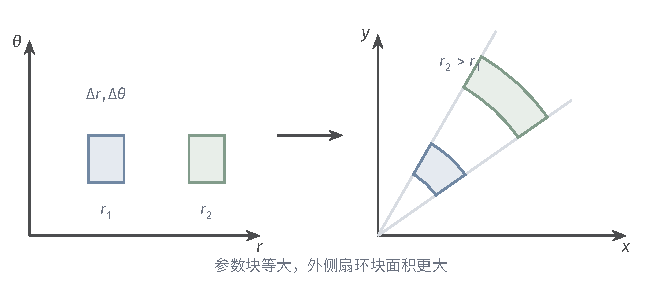
\includegraphics[width=112mm]{figures/00-shared/mathematical-preliminaries-upper/00-shared/tikz/mathematical-language-combinatorics-analysis-optimization-comprehension-additions/polar-area-weight.pdf}
\caption{同样的径向宽度和角度宽度，在较大半径处产生更大的面积。一阶面积为$r\Delta r\Delta\theta$，由此得到极坐标权重。}
\label{fig:vol3-classical-polar-weight}
\end{figure}

原点处行列式为零，角度的两端又表示同一条射线，因此不能把闭参数矩形直接代入上述双射定理。可以先限制$r\geq\varepsilon$且$\varepsilon\leq\theta\leq2\pi-\varepsilon$，在紧截断区域上换元，再令$\varepsilon\downarrow0$。对于圆盘上的连续函数，被去掉的小圆盘和窄扇区的贡献受函数上界乘面积控制，趋于零；参数侧的遗漏也由有界权重控制。

例如半径$R$的圆盘面积为
\[
 \int_0^{2\pi}\int_0^R r\,\mathrm dr\,\mathrm d\theta=\pi R^2.
\]
若角度取到$4\pi$，内部被覆盖两次，结果也变成两倍。对于有奇点的被积函数，不能只用“接缝不贡献面积”来跳过极限估计。

柱坐标保留高度$z$，即在极坐标后加上第三个坐标，其体积权重仍含$r$：
\[
 \mathrm dV=r\,\mathrm dr\,\mathrm d\theta\,\mathrm dz.
\]
因此半径$R$、高度$H$的圆柱体积为$\pi R^2H$。轴线和角度接缝通过与极坐标相同的截断处理。

球坐标使用距原点的距离$\rho$、从正$z$轴量起的极角$\varphi$和方位角$\theta$：
\[
 T(\rho,\varphi,\theta)
 =(\rho\sin\varphi\cos\theta,\rho\sin\varphi\sin\theta,\rho\cos\varphi).
\]
三个局部正交方向的长度比例分别是$1$、$\rho$和$\rho\sin\varphi$，也可直接计算Jacobian行列式验证。因此
\[
 \mathrm dV=\rho^2\sin\varphi\,\mathrm d\rho\,\mathrm d\varphi\,\mathrm d\theta.
\]

在$\rho>0$、$0<\varphi<\pi$及一个长度为$2\pi$的开角度区间内，映射单次覆盖去掉轴线和接缝后的空间。计算球内连续函数的积分时，先截去原点、极轴附近及接缝附近的小区域，再以有界性估计遗漏。球体积由此为
\[
 \int_0^{2\pi}\int_0^\pi\int_0^R
 \rho^2\sin\varphi\,\mathrm d\rho\,\mathrm d\varphi\,\mathrm d\theta
 =\frac{4\pi R^3}{3}.
\]

\subsection{线性换元与积分结果的核对}

线性变换可以把斜区域变成坐标盒。

设$D$由$0\leq x+y\leq2$和$0\leq x-y\leq2$围成，求$\int_D(x+y)\,\mathrm d(x,y)$。令$u=x+y$、$v=x-y$，则参数区域为$[0,2]^2$，逆变换为
\[
 x=(u+v)/2,
\]
\[
 y=(u-v)/2.
\]
其行列式为$-1/2$，故面积权重为$1/2$。于是
\[
 \int_D(x+y)\,\mathrm d(x,y)
 =\int_0^2\int_0^2\frac u2\,\mathrm du\,\mathrm dv=2.
\]
取被积函数为$1$，同样得到区域面积$2$；原被积函数在对称区域上的平均值为$1$，两者相乘也为$2$。这同时核验了区域、权重和积分值。

\section{参数积分}

若密度或被积函数还依赖一个参数，积分便定义了新的函数。

判断它是否连续、能否求导，需要控制整个积分区域上的变化，逐点成立的极限本身不够。本节固定紧Jordan区域$D$，用连续性提供统一控制。

\subsection{固定区域上的参数积分与连续性}

设$K$为紧参数区域，$f$在$D\times K$上连续，记
\[
 F(\bm t)=\int_D f(\bm x,\bm t)\,\mathrm d\bm x.
\]
乘积紧集上的一致连续性使$\sup_{\bm x\in D}|f(\bm x,\bm t)-f(\bm x,\bm s)|$在$\bm t\to\bm s$时趋于零。因此
\[
 |F(\bm t)-F(\bm s)|
 \leq |D|\sup_{\bm x\in D}|f(\bm x,\bm t)-f(\bm x,\bm s)|\longrightarrow0.
\]
这证明了连续性。参数区域不必整体有界：讨论一个内点附近时，取包含该点的小闭盒即可。

\subsection{积分号下的偏导数与全微分}

现在设参数属于开集，$f$和各参数偏导$\partial_{t_j}f$在$D$与参数邻域的乘积上连续。固定一个参数点和足够小的闭邻域，一元中值定理把差商写成附近参数处的偏导值。偏导的一致连续性说明差商对全部$\bm x\in D$一致趋于$\partial_{t_j}f$；对差取积分并用上面的上确界估计，便得到
\begin{equation}
 \partial_{t_j}F(\bm t)=\int_D\partial_{t_j}f(\bm x,\bm t)\,\mathrm d\bm x.
\label{eq:classical-differentiate-under-integral}
\end{equation}
右侧又是连续参数积分，故所有参数偏导连续，$F$是$C^1$函数。它的全微分为
\[
 DF_{\bm t}[\bm h]=\int_D D_{\bm t}f(\bm x,\bm t)[\bm h]\,\mathrm d\bm x.
\]

这里先获得偏导，再由连续偏导判据得到整体可微；不能只证明每个方向上的极限就略去这一步。

例如$F(t)=\int_0^1 e^{tx}\,\mathrm dx$，在任意有界参数区间上都满足这些条件，故$F'(0)=\int_0^1x\,\mathrm dx=1/2$，无需在$t=0$处处理显式表达式的可去奇点。

\subsection{变限参数积分}

积分区间也随参数变化时，积分值的变化有两部分：原区间内部函数改变，以及两端新添或移除的细条。

设$a(t),b(t)$为$C^1$函数，$f(x,t)$及$\partial_tf(x,t)$在所需区间附近连续。将积分写为固定基点到$b(t)$的积分减去固定基点到$a(t)$的积分，再用链式法则，得到
\[
 \frac{\mathrm d}{\mathrm dt}\int_{a(t)}^{b(t)}f(x,t)\,\mathrm dx
 =\int_{a(t)}^{b(t)}\partial_tf(x,t)\,\mathrm dx
 +f(b(t),t)b'(t)-f(a(t),t)a'(t).
\]

上端向右移动增加积分，下端向右移动减少积分，所以两个边界项符号相反。多个参数时逐一求偏导，或将$a'$、$b'$和$\partial_tf$换成作用于同一参数增量的全微分。更一般的移动区域会产生沿边界的贡献；本章只在上述区间变限和已明确参数化的区域上使用这一规则。

\par\Needspace{10\baselineskip}
\section{路径积分}
\label{sec:multivariable-path-integration}

区域积分累计的是铺满一块区域的量，许多问题却只沿一条曲线累计。一根弯曲细铁丝的质量由各处的线密度和铁丝长度决定；把物体沿一条路线推过去，推力做的功不仅取决于力的大小和路线长度，还取决于力与前进方向的夹角。
两类问题都沿曲线累计，被积对象却不同：线密度在每一点只给出一个数，是标量函数；力在每一点给出一个带方向的量，是向量场。

相应地有两种路径积分。第一类路径积分把曲线切成小段，用每段上的函数值乘这段的实际长度再相加，铁丝质量就是这样算出的；它不关心沿哪个方向走过曲线。
第二类路径积分在每一小段上先取力与这段有向位移的内积，只保留力沿前进方向的分量，再把这些数相加；反向行走时每段位移都反号，积分也随之变号。

两种积分都要先用参数描述曲线，因此本节先说明路径与弧长，再分别讨论两类积分的定义、性质和计算。
最后研究力沿路径做的功什么时候只取决于起点和终点、而与中间的路线无关，这对应物理中保守力与势能的关系。
本节的参数积分都是一元Riemann积分\scite{math-openstax-calculus3}。

\subsection{参数路径与弧长}
\label{sec:multivariable-line-integrals}

描述一次行进，需要知道每个时刻所在的位置。位置随时间连续变化，就得到一条路径；位置对时间的导数是速度，速度的大小称为速率。速率恒定时，速率乘经过的时间就是走过的路程。
本小节先给出路径的定义，再用折线逼近说明：速率随时间变化时，路程等于速率对时间的积分。

\subsubsection{路径的定义}

\paragraph{参数化路径}

不妨把参数$t$看成时间，把$\gamma(t)$看成一个质点在时刻$t$所在的位置。同一组位置可以走得快或慢，可以从任一端出发，也可以来回走好几遍；只记下经过了哪些点，就会丢失这些信息。

用区间到空间的连续映射描述行进过程，位置和先后次序就一起保留了下来。
\begin{definition}[路径]
设$a<b$。连续映射$\gamma:[a,b]\to\mathbb R^d$称为一条\term{路径}（path），$\gamma(a)$和$\gamma(b)$分别为起点和终点；若两者相等，称为闭路径。
集合$C=\gamma([a,b])$称为路径的像。
\end{definition}

像集$C$只记录质点经过的位置，参数$t$还规定了经过的先后次序，所以同一个像集可以对应行进方式完全不同的路径。
\begin{example}[同一条对角线段上的三条路径]
\label{ex:analysis-diagonal-segment-paths}
以下三条平面路径的像都是连接$(0,0)$与$(1,1)$的对角线段：
\begin{itemize}
 \item $\gamma(t)=(t,t)^\top$，$0\leq t\leq1$，从$(0,0)$走到$(1,1)$，速度为$(1,1)^\top$；
 \item $\eta(u)=(u/2,u/2)^\top$，$0\leq u\leq2$，同样从$(0,0)$走到$(1,1)$，速度减半为$(1/2,1/2)^\top$，用时加倍；
 \item $\rho(t)=(t,t)^\top$（$0\leq t\leq1$）、$\rho(t)=(2-t,2-t)^\top$（$1\leq t\leq2$），先走到$(1,1)$再原路返回。
\end{itemize}
$\gamma$与$\eta$只是快慢不同，线段上每个点都恰好经过一次。$\rho$的像仍是这条线段，但每个内点被经过两次：去程一次，回程一次。
\end{example}

后面会看到，两种路径积分对$\gamma$与$\eta$都给出相同结果；沿$\rho$按长度累计时，结果是沿$\gamma$的两倍，按有向位移累计时，去程与回程恰好抵消。
可见路径积分是沿“一次行进”定义的，只知道像集还不能确定它。要计算一根铁丝的质量，应选一条把铁丝恰好走一遍的路径。

\paragraph{分段光滑路径}

示例~\ref{ex:analysis-diagonal-segment-paths}中的往返路径$\rho$在$t=1$处突然掉头，正方形边界在四个角处突然转向。这些位置没有唯一的切线方向，但在每一段直线上速度都存在且连续。为了把折线、多边形边界这类常见路径纳入计算，允许路径在有限个参数点处分段。
\begin{definition}[分段光滑路径]
若存在分割$a=t_0<t_1<\cdots<t_n=b$，使$\gamma$在每个$[t_{j-1},t_j]$上为$C^1$映射，称$\gamma$为分段$C^1$路径，也称分段光滑路径。
若每段内部还满足$\gamma'(t)\neq\bm0$，称该路径分段正则。
\end{definition}

这里“在闭区间$[t_{j-1},t_j]$上为$C^1$”是指该段内部的导数连续，并能连续延拓到该段的两个端点；相邻两段在公共端点处的导数不必相同。
例如$\rho$在$[0,1]$上的速度为$(1,1)^\top$，在$[1,2]$上的速度为$(-1,-1)^\top$。两段在$t=1$处的速度不同，但各自连续，所以$\rho$是分段$C^1$路径。

本节的路径积分都在分段$C^1$路径上定义。折点只有有限个，而改变有界函数在有限个点的取值不影响Riemann积分，所以折点处的速度取什么值不影响参数积分。
分段正则要求每段内部速度不为零，排除了质点在某段中途停住的情形。本节的积分并不要求路径正则；后面用到单位切向量时，只在速度非零处使用它。

\subsubsection{路径的长度}

\paragraph{弧长}

测量一条弯曲道路的长度时，可以在路上依次插几根标杆，量出相邻标杆之间的直线距离再相加。每段直线距离都不超过对应那段路的实际长度，所以这样得到的折线长度不会超过道路长度；在两根标杆之间再插一根，由三角不等式，新折线的长度不会变短。标杆越密，折线越贴近道路，因此把实际长度定义为所有内接折线长度的上确界。
\begin{definition}[路径的弧长]
路径$\gamma:[a,b]\to\mathbb R^d$的弧长定义为
\[
 \ell(\gamma)=\sup_{a=t_0<\cdots<t_n=b}
 \sum_{j=1}^n\lVert\gamma(t_j)-\gamma(t_{j-1})\rVert_2.
\]
上确界取遍$[a,b]$的全部有限分割；若此值有限，称路径可求长。
\end{definition}

这个定义只用到路径上点的位置，不需要导数，所以任何连续路径都可以讨论它是否可求长。

对分段光滑路径，弧长还可以用速度直接计算。在一小段参数区间$[t_{j-1},t_j]$上，质点的位移近似为速度乘时间：
$\gamma(t_j)-\gamma(t_{j-1})\approx\gamma'(t_{j-1})(t_j-t_{j-1})$，
所以这一小段的长度近似为速率$\lVert\gamma'(t_{j-1})\rVert_2$乘时间，汽车里程表正是这样累计路程的。把这些乘积相加并令分割变细，就得到下面的公式。
\begin{theorem}[分段光滑路径的弧长]
若$\gamma:[a,b]\to\mathbb R^d$分段$C^1$，则它可求长，且
\[
 \ell(\gamma)=\int_a^b\lVert\gamma'(t)\rVert_2\,\mathrm dt.
\]
\end{theorem}
\begin{proof}
加入分点不会使折线变短，所以计算上确界时只需考虑包含全部折点的分割；这样的折线长度按光滑段相加，弧长也按段相加。因此只需在一段$C^1$区间上证明，再把各段的等式相加。证明分两步：先说明任何折线都不比速度积分长，再说明足够细的折线与速度积分相差任意小。

第一步。对该段中的$\alpha<\beta$，由各坐标分量的一元基本定理，
$\gamma(\beta)-\gamma(\alpha)=\int_\alpha^\beta\gamma'(t)\,\mathrm dt$，这里向量的积分表示对各分量分别积分。
若弦$\gamma(\beta)-\gamma(\alpha)$非零，取它方向上的单位向量$\bm u$，则由Cauchy--Schwarz不等式
\[
 \lVert\gamma(\beta)-\gamma(\alpha)\rVert_2
 =\bm u^\top\bigl(\gamma(\beta)-\gamma(\alpha)\bigr)
 =\int_\alpha^\beta\bm u^\top\gamma'(t)\,\mathrm dt
 \leq\int_\alpha^\beta\lVert\gamma'(t)\rVert_2\,\mathrm dt;
\]
弦为零时这个不等式直接成立。同样的推理说明，任何连续向量值函数$\bm v$都满足$\lVert\int_\alpha^\beta\bm v\,\mathrm dt\rVert_2\leq\int_\alpha^\beta\lVert\bm v\rVert_2\,\mathrm dt$。
对任意分割把各段弦长相加，可知任意内接折线的长度都不超过$\int_a^b\lVert\gamma'\rVert_2\,\mathrm dt$，所以上确界也不超过它。

第二步。$\gamma'$在紧区间上一致连续。给定$\varepsilon>0$，取足够细的分割，使每个小区间上任意两点的$\gamma'$相距小于$\varepsilon$，并记$\Delta t_j=t_j-t_{j-1}$。
在第$j$个小区间上，
\[
 \gamma(t_j)-\gamma(t_{j-1})-\gamma'(t_{j-1})\Delta t_j
 =\int_{t_{j-1}}^{t_j}\bigl(\gamma'(t)-\gamma'(t_{j-1})\bigr)\,\mathrm dt,
\]
由第一步的范数不等式，它的范数不超过$\varepsilon\Delta t_j$；于是这一段的弦长与$\lVert\gamma'(t_{j-1})\rVert_2\Delta t_j$之差不超过$\varepsilon\Delta t_j$。
同一小区间上，$\int\lVert\gamma'\rVert_2\,\mathrm dt$与$\lVert\gamma'(t_{j-1})\rVert_2\Delta t_j$的差也不超过$\varepsilon\Delta t_j$。
两项相加后对$j$求和，速度积分与这条折线长度的差不超过$2\varepsilon(b-a)$，所以上确界不小于速度积分减$2\varepsilon(b-a)$。令$\varepsilon\downarrow0$，得到反向不等式。
\end{proof}

用这个公式可以计算示例~\ref{ex:analysis-diagonal-segment-paths}中三条路径的长度，并检验圆周长公式。
\begin{example}[对角线段与圆周的弧长]
对角线段$\gamma(t)=(t,t)^\top$，$0\leq t\leq1$，速度为$(1,1)^\top$，速率为$\sqrt2$，所以$\ell(\gamma)=\int_0^1\sqrt2\,\mathrm dt=\sqrt2$。两个坐标各变化$1$，走过的距离却不是$1+1=2$，而是斜边的长度。

慢速路径$\eta$的速率为$\sqrt2/2$，用时为$2$，长度为$\int_0^2(\sqrt2/2)\,\mathrm du=\sqrt2$。往返路径$\rho$在两段上的速率都是$\sqrt2$，总用时为$2$，长度为$2\sqrt2$。

半径为$r$的圆周可以参数化为$t\mapsto(r\cos t,r\sin t)^\top$，$0\leq t\leq2\pi$。速度为$(-r\sin t,r\cos t)^\top$，速率恒为$r$，长度为$\int_0^{2\pi}r\,\mathrm dt=2\pi r$，与圆周长公式一致。
\end{example}

$\gamma$与$\eta$的长度相同，因为速率减半恰好被用时加倍抵消；$\rho$的长度是$\gamma$的两倍，因为弧长把经过的次数也计算在内。

记$s(t)=\int_a^t\lVert\gamma'(u)\rVert_2\,\mathrm du$为截至时刻$t$累计走过的路程，它就是里程表在时刻$t$的读数。在每个光滑段内部，$s$对$t$的导数是速率$\lVert\gamma'(t)\rVert_2$，因此常把长度权重简写为
$\mathrm ds=\lVert\gamma'(t)\rVert_2\,\mathrm dt$，读作“一小段时间$\mathrm dt$内走过的一小段路程”。

\subsection{第一类路径积分}

第一类路径积分的被积对象是定义在曲线上的标量函数，例如铁丝各处的线密度或一条道路沿线各处的温度。每一小段的贡献是函数值乘这一小段的实际长度，因此它只需要路程这一个权重，不涉及方向。

\subsubsection{定义与可积性}

\paragraph{按弧长的积分}

设一根铁丝沿路径$\gamma$放置，$h(\bm x)$是它在点$\bm x$处的线密度，即单位长度的质量。线密度为常数时，质量等于密度乘长度；密度随位置变化时，把铁丝切成许多小段，每段上的密度近似为常数。
在参数小区间$[t_{j-1},t_j]$对应的一段上取一个时刻$\xi_j$，这段的质量约为
\[
 h(\gamma(\xi_j))\,\lVert\gamma'(\xi_j)\rVert_2\,(t_j-t_{j-1}),
\]
即“该处密度”乘“该段长度”。把各段相加，就得到参数区间上函数$h(\gamma(t))\lVert\gamma'(t)\rVert_2$的积分和，所以用这个函数的一元积分定义沿路径的累计。这里先讨论沿路径连续的密度；有限分段连续的密度可逐段处理。
\begin{definition}[第一类路径积分]
设$\gamma:[a,b]\to\mathbb R^d$分段$C^1$，$h$在路径像集上连续。定义\term{第一类路径积分}为
\begin{equation}
 \int_\gamma h\,\mathrm ds=\int_a^b h(\gamma(t))\|\gamma'(t)\|_2\,\mathrm dt.
 \label{eq:analysis-scalar-line-integral}
\end{equation}
右侧按各光滑段的一元Riemann积分相加，因被积函数分段连续而存在。
\end{definition}

这个积分有几种常见读法。取$h=1$，积分就是弧长$\ell(\gamma)$；$h$是非负线密度时，积分是铁丝的总质量。

若$\ell(\gamma)>0$，比值
\[
 \bar h=\frac1{\ell(\gamma)}\int_\gamma h\,\mathrm ds
\]
是$h$沿曲线按长度的平均值：沿一条道路每隔相同路程记录一次温度再求平均，记录越密，结果越接近$\bar h$。
这里的平均按路程加权，而不按参数时间加权。若一辆车在某段路上开得很慢，按时间平均会让这段路的温度占更大比重，按路程平均则不受车速影响。

用一根密度不均匀的半圆铁丝可以说明质量和平均线密度的计算。
\begin{example}[上半圆铁丝的质量与平均线密度]
\label{ex:analysis-semicircle-wire}
沿上半单位圆$\gamma(t)=(\cos t,\sin t)^\top$，$0\leq t\leq\pi$，放一根铁丝，线密度为$h(x,y)=y$，即越高的地方越重。速度为$(-\sin t,\cos t)^\top$，速率恒为$1$，所以总质量为
\[
 \int_\gamma y\,\mathrm ds=\int_0^\pi\sin t\,\mathrm dt=2.
\]
铁丝长度为$\pi$，平均线密度为$\bar h=2/\pi\approx0.64$。两端$(\pm1,0)$处密度为零，顶点$(0,1)$处密度为$1$，平均值落在两者之间。
\end{example}
这条参数化的速率恒为$1$，参数时间与路程同步增长，所以按时间平均也得到$2/\pi$；速率不恒定时，两种平均一般不同。

连续密度在紧路径像集上有界，因而积分的绝对值不超过密度绝对值的上界乘弧长。路径积分按曲线上的实际取值累计，不能用区域平均值代替沿线的密度。

\subsubsection{积分的基本性质}

下面各条性质中的有符号函数都假设沿所讨论的路径可积。把定义式~\eqref{eq:analysis-scalar-line-integral}代入一元Riemann积分的相应性质，就逐项得到这些结论；用铁丝质量来读，每条性质都有直接的含义。

\paragraph{加法}

若$h,k$沿$\gamma$可积，则$h+k$也沿$\gamma$可积，且
\[
 \int_\gamma(h+k)\,\mathrm ds=\int_\gamma h\,\mathrm ds+\int_\gamma k\,\mathrm ds.
\]
绝对可积性由$|h+k|\leq|h|+|k|$保证，等式来自一元积分的加法。若铁丝由两种材料叠合而成，总质量等于两种材料各自的质量之和。

\paragraph{减法}

把$k$换成$-k$，它同样沿$\gamma$可积，由加法得到
\[
 \int_\gamma(h-k)\,\mathrm ds=\int_\gamma h\,\mathrm ds-\int_\gamma k\,\mathrm ds.
\]
两个积分都是有限数，所以相减时不会出现$\infty-\infty$。

\paragraph{数乘}

若$c\in\mathbb R$且$h$沿$\gamma$可积，则
\[
 \int_\gamma ch\,\mathrm ds=c\int_\gamma h\,\mathrm ds.
\]
把每一小段上的密度同时放大$c$倍，总质量也放大$c$倍。

\paragraph{路径拼接}

若$\gamma_1$的终点是$\gamma_2$的起点，记先走$\gamma_1$、再走$\gamma_2$的拼接路径为$\gamma_1*\gamma_2$。$h$沿两条路径分别可积时，
\[
 \int_{\gamma_1*\gamma_2}h\,\mathrm ds
 =\int_{\gamma_1}h\,\mathrm ds+\int_{\gamma_2}h\,\mathrm ds.
\]
拼接路径的参数区间由两段参数区间首尾相接而成，等式来自一元积分对区间的可加性。逐段计算折线和多边形边界上的积分，依据的正是这个等式。

两段路径有重叠部分时，重叠部分的贡献会计入两次。示例~\ref{ex:analysis-diagonal-segment-paths}中的往返路径$\rho$由去程$\gamma$与原路返回的一段拼成；返回段$(2-t,2-t)^\top$，$1\leq t\leq2$，经换元$u=2-t$化为$\gamma$上的同一个积分，所以沿$\rho$的积分是沿$\gamma$的两倍。

\paragraph{重参数化与方向无关}

同一根铁丝无论从哪一端开始称量、量得快还是慢，质量都不变。数学上，改变快慢和方向都可以用换参数表示：设$t=\sigma(u)$是两个参数区间之间单调、端点相配的分段$C^1$微分同胚，新路径$\gamma\circ\sigma$在“时刻”$u$位于$\gamma(\sigma(u))$。
链式法则给出新速度$(\gamma\circ\sigma)'(u)=\gamma'(\sigma(u))\sigma'(u)$，所以新速率为
$\lVert\gamma'(\sigma(u))\rVert_2|\sigma'(u)|$。代入定义并用一元换元公式$t=\sigma(u)$，得到
\[
 \int_{\gamma\circ\sigma}h\,\mathrm ds=\int_\gamma h\,\mathrm ds.
\]

走得慢时速率变小，但用时按同一比例变长，乘积不变。$\sigma$递减时路径反向，绝对值$|\sigma'|$仍给出非负的长度权重，所以反向行进也不改变第一类积分。
在示例~\ref{ex:analysis-diagonal-segment-paths}中，$\eta=\gamma\circ\sigma$，其中$\sigma(u)=u/2$，$0\leq u\leq2$，所以沿$\eta$与沿$\gamma$的第一类积分相同，弧长都是$\sqrt2$。换参数只改变快慢和方向，不改变经过的次数，所以往返路径$\rho$不是$\gamma$的重参数化。

\paragraph{单调性}

若在路径上处处有$h\leq k$，则
\[
 \int_\gamma h\,\mathrm ds\leq\int_\gamma k\,\mathrm ds.
\]
这是因为长度权重$\lVert\gamma'\rVert_2$非负，被积函数的大小关系乘以权重后保持不变。密度处处较小的铁丝，总质量也较小。

\paragraph{绝对值不等式}

由一元积分的绝对值不等式可得
\[
 \left|\int_\gamma h\,\mathrm ds\right|
 \leq\int_\gamma|h|\,\mathrm ds
 \leq\sup_C|h|\,\ell(\gamma).
\]
$h$有界时，最后一个不等式给出有限的上界：累计量的绝对值不超过函数绝对值的上确界乘路径长度。例如在示例~\ref{ex:analysis-semicircle-wire}中，密度$y$不超过$1$，质量$2$确实不超过$1\cdot\pi$。

\subsubsection{积分的计算}

计算第一类路径积分分三步：给曲线选一条把它恰好走一遍的参数化；把$h(\gamma(t))$乘速率$\lVert\gamma'(t)\rVert_2$；在参数区间上做一元积分，有折点时在折点两侧分别计算再相加。
先在示例~\ref{ex:analysis-diagonal-segment-paths}的对角线段上积分一个线性函数。
\begin{example}[沿对角线段积分$x+y$]
取$\gamma(t)=(t,t)^\top$，$0\leq t\leq1$，$h(x,y)=x+y$。沿路径有$h(\gamma(t))=2t$，速率为$\sqrt2$，所以
\[
 \int_\gamma h\,\mathrm ds=\int_0^1 2t\cdot\sqrt2\,\mathrm dt=\sqrt2.
\]
线段长为$\sqrt2$，平均值为$\sqrt2/\sqrt2=1$，恰是$h$在线段中点$(1/2,1/2)$的值，因为$h$沿这条线段随路程线性变化。
\end{example}
若漏掉速率而只计算$\int_0^12t\,\mathrm dt=1$，得到的是按参数时间的累计，比按长度的累计少了速率因子$\sqrt2$。第一类路径积分也不是线段下方某块平面区域的面积：区域积分按面积加权，这里的权重是沿线段的长度。

许多平面曲线写成函数图像$y=\psi(x)$。

设$\psi$在$[a,b]$上为$C^1$，沿$x$递增的图像路径$\gamma(x)=(x,\psi(x))^\top$，$a\leq x\leq b$，以$x$本身作参数，速度为$(1,\psi'(x))^\top$，于是
\[
 \int_\gamma h\,\mathrm ds
 =\int_a^b h(x,\psi(x))\sqrt{1+\psi'(x)^2}\,\mathrm dx.
\]
根号是图像路径的速率：自变量前进$\mathrm dx$时，曲线同时升高约$\psi'(x)\,\mathrm dx$，斜边长约为$\sqrt{1+\psi'(x)^2}\,\mathrm dx$。曲线越陡，同一个$\mathrm dx$对应的路程越长，因此不能只写$\mathrm dx$。

用这个公式可以计算一段抛物线铁丝的质量。
\begin{example}[抛物线铁丝的质量]
沿抛物线段$y=x^2$，$0\leq x\leq1$，放一根铁丝，线密度为$h(x,y)=x$。这里$\psi(x)=x^2$，$\psi'(x)=2x$，速率为$\sqrt{1+4x^2}$。令$w=1+4x^2$，则$\mathrm dw=8x\,\mathrm dx$，$w$从$1$变到$5$，所以
\[
 \int_\gamma x\,\mathrm ds=\int_0^1x\sqrt{1+4x^2}\,\mathrm dx
 =\frac18\int_1^5\sqrt w\,\mathrm dw=\frac{5\sqrt5-1}{12}\approx0.85.
\]
\end{example}
若漏写根号，只会得到$\int_0^1x\,\mathrm dx=1/2$，丢掉了曲线变陡后多出的长度。

\subsection{第二类路径积分}

第一类积分只问“每段有多长”，做功问题还要问“这段朝哪个方向走”。推一辆车时，力与前进方向一致才完全用于推动，力与前进方向垂直时不做功，力与前进方向相反时做负功。描述这种累计，需要先说明“每一点有一个力”是什么意思。

\subsubsection{定义与可积性}

\paragraph{向量场}

力在空间中随位置变化：地面附近的重力处处竖直向下，太阳对行星的引力指向太阳且随距离减弱。河流中的水在每一点有一个流速，流速同样带有大小和方向。这类对象在每个位置给出一个与位置同维的向量。
\begin{definition}[向量场]
设$U\subseteq\mathbb R^d$。映射$\bm F:U\to\mathbb R^d$称为$U$上的\term{向量场}（vector field）。
\end{definition}

向量场的输入是位置，输出是放在该位置的一个向量，常画成从该点出发的箭头。下面是三个平面例子：
\begin{itemize}
 \item 常向量场$\bm F(x,y)=(0,-mg)^\top$描述地面附近质量为$m$的物体所受重力，其中$g$是重力加速度，箭头处处竖直向下、长度相同；
 \item $\bm F(x,y)=(x,y)^\top$的箭头从原点向外，离原点越远越长；
 \item $\bm F(x,y)=(-y,x)^\top$的箭头与以原点为圆心的圆相切，按逆时针方向，长度等于到原点的距离。它是绕原点以角速度$1$旋转的圆盘上各点的速度，本节称它为旋转场。
\end{itemize}
旋转场与位置向量处处垂直，因为$(-y)\cdot x+x\cdot y=0$。

\paragraph{有向线积分}

先看最简单的情形：常力$\bm F$把物体沿直线移动了位移$\Delta\bm r$。中学物理中的功是$\lVert\bm F\rVert_2\lVert\Delta\bm r\rVert_2\cos\theta$，其中$\theta$是力与位移的夹角，它正是内积$\bm F^\top\Delta\bm r$。把力分解为沿位移方向和垂直于位移方向的两部分，只有前一部分做功：$\theta<\pi/2$时功为正，$\theta=\pi/2$时为零，$\theta>\pi/2$时为负。

路线弯曲、力随位置变化时，把路径切成许多小段。参数小区间$[t_{j-1},t_j]$上的位移近似为$\gamma'(\xi_j)(t_j-t_{j-1})$，力近似为常力$\bm F(\gamma(\xi_j))$，这段的功约为
\[
 \bm F(\gamma(\xi_j))^\top\gamma'(\xi_j)\,(t_j-t_{j-1}).
\]
各段相加就是参数区间上函数$\bm F(\gamma(t))^\top\gamma'(t)$的积分和。这里乘的是速度向量本身，不是速率，所以位移的方向保留在被积函数中。
\begin{definition}[第二类路径积分]
设$\gamma:[a,b]\to U$分段$C^1$，$\bm F:U\to\mathbb R^d$为向量场。
若$\bm F$在路径像集上连续，定义\term{第二类路径积分}（vector line integral）为
\begin{equation}
 \int_\gamma\bm F\mathbin{\cdot}\mathrm d\bm r
 =\int_a^b\bm F(\gamma(t))^\top\gamma'(t)\,\mathrm dt.
 \label{eq:analysis-vector-line-integral}
\end{equation}
\end{definition}

记号$\mathrm d\bm r$表示一小段有向位移$\gamma'(t)\,\mathrm dt$，$\bm F\cdot\mathrm d\bm r$是这一小段上的功。
在平面中，若$\bm F=(P,Q)^\top$，路径为$\gamma(t)=(x(t),y(t))^\top$，则被积函数是$P\,x'(t)+Q\,y'(t)$，因此积分也写成$\int_\gamma P\,\mathrm dx+Q\,\mathrm dy$：$P\,\mathrm dx$是力的水平分量在水平位移上做的功，$Q\,\mathrm dy$是竖直分量在竖直位移上做的功。三维中再加上第三个分量$R$对应的$R\,\mathrm dz$。

若$\bm F$在路径像集上连续，复合函数$\bm F\circ\gamma$在各光滑段上连续，被积函数在紧参数区间上有界，所以参数积分绝对可积。

两类路径积分可以用单位切向量联系起来。在速度非零处，单位切向量$\bm\tau=\gamma'/\lVert\gamma'\rVert_2$指向前进方向，于是
\[
 \bm F^\top\gamma'\,\mathrm dt=(\bm F^\top\bm\tau)\,\lVert\gamma'\rVert_2\,\mathrm dt=(\bm F^\top\bm\tau)\,\mathrm ds.
\]
$\bm F^\top\bm\tau$是力在前进方向上的分量，称为切向分量。速度为零处，左侧的被积函数为零，右侧的长度权重$\lVert\gamma'\rVert_2$也为零，不必定义$\bm\tau$。所以第二类积分等于切向分量的第一类积分：功等于“沿前进方向的力”乘“走过的路程”再累计。
区别在于，切向分量依赖于行进方向：反向行走时$\bm\tau$变为$-\bm\tau$，切向分量变号，积分也变号；而第一类积分的被积函数与方向无关。

若$\bm F$是流体的速度场，沿闭路径的积分累计的是流速沿这条闭路径的切向分量，称为\term{环流}（circulation）。环流为正，表示流体总体上倾向于沿所选方向绕这条闭路径流动。
例如沿单位圆逆时针行进时，旋转场$(-y,x)^\top$的切向分量处处为$1$，一周的环流是$1\times2\pi=2\pi$。

图~\ref{fig:analysis-process-line-density-work}用同一条线段对照两类积分：左图按长度累计常数密度，右图只累计位移的水平分量。
\begin{figure}[!htbp]
 \centering
 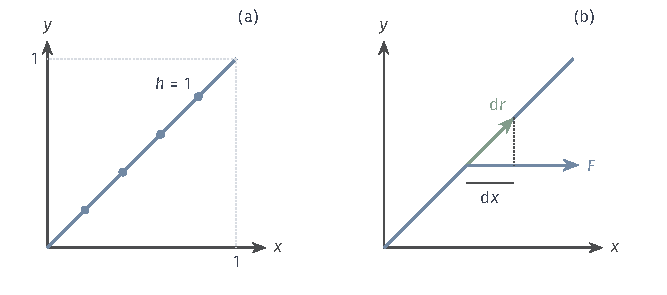
\includegraphics[width=112mm]{figures/00-shared/mathematical-preliminaries-upper/00-shared/tikz/chapter3-concept-processes/line-density-work.pdf}
 \caption{路径均为$\gamma(t)=(t,t)^\top$，$0\leq t\leq1$。(a) 常数线密度$h=1$按弧长累计，得到$\sqrt2$。(b) 常向量场$\bm F=(1,0)^\top$只取位移的水平分量，做功为$1$；图中$\mathrm dx$是$\mathrm d\bm r$的水平投影。相同路径、不同被积对象和权重给出不同积分。}
 \label{fig:analysis-process-line-density-work}
\end{figure}

\subsubsection{积分的基本性质}

下列公式均由内积的线性和一元Riemann积分的相应性质得到。以下说$\bm F$沿$\gamma$可积，是指沿各段满足前述连续性条件，因而相应的有向积分有限。前三条说明功对力是线性的，接下来三条说明功怎样随路径的拼接、方向和参数化变化，最后一条估计功的大小。

\paragraph{加法}

若$\bm F$和$\bm G$沿$\gamma$可积，则$\bm F+\bm G$也沿$\gamma$可积，且
\[
 \int_\gamma(\bm F+\bm G)\cdot\mathrm d\bm r
 =\int_\gamma\bm F\cdot\mathrm d\bm r+\int_\gamma\bm G\cdot\mathrm d\bm r.
\]
这里先把两个向量场相加，再与位移取内积。两个力同时作用时，合力做的功等于两个力各自做功之和。

\paragraph{减法}

把$\bm G$换成相反场$-\bm G$，由加法得到
\[
 \int_\gamma(\bm F-\bm G)\cdot\mathrm d\bm r
 =\int_\gamma\bm F\cdot\mathrm d\bm r-\int_\gamma\bm G\cdot\mathrm d\bm r.
\]
可积性保证两个积分都有限，所以可以相减。

\paragraph{数乘}

对实数$c$，有
\[
 \int_\gamma c\bm F\cdot\mathrm d\bm r
 =c\int_\gamma\bm F\cdot\mathrm d\bm r.
\]
力放大$c$倍，功也放大$c$倍；$c<0$时力反向，功变号。路径本身没有改变。

\paragraph{路径拼接}

若$\gamma_1$和$\gamma_2$首尾相接，则
\[
 \int_{\gamma_1*\gamma_2}\bm F\cdot\mathrm d\bm r
 =\int_{\gamma_1}\bm F\cdot\mathrm d\bm r
 +\int_{\gamma_2}\bm F\cdot\mathrm d\bm r.
\]
先走一段再走一段，总功是两段的功之和。因此分段光滑路径可以逐段计算，但每段都必须按这次行进的实际方向参数化。

\paragraph{方向反转}

记反向路径为$\gamma^{-}(u)=\gamma(a+b-u)$，$a\leq u\leq b$，它从$\gamma(b)$出发、沿原路走回$\gamma(a)$。由链式法则，它的速度是$-\gamma'(a+b-u)$，与原速度相反；再用一元换元$t=a+b-u$，得到
\[
 \int_{\gamma^{-}}\bm F\cdot\mathrm d\bm r
 =-\int_\gamma\bm F\cdot\mathrm d\bm r.
\]
顺风骑车时风做正功，沿原路逆风骑回来，风在每一段都做等量的负功。第一类积分反向后不变，因为长度始终非负；有向位移反向则改变符号。
特别地，往返路径$\gamma*\gamma^{-}$上的第二类积分为零，而它的长度是$\gamma$的两倍；示例~\ref{ex:analysis-diagonal-segment-paths}中的$\rho$就是对角线段上的这种往返路径。

\paragraph{重参数化}

若$t=\sigma(u)$为端点相配、严格递增的分段$C^1$微分同胚，则
$(\gamma\circ\sigma)'(u)=\gamma'(\sigma(u))\sigma'(u)$。在参数公式中应用换元$t=\sigma(u)$，得到
\[
 \int_{\gamma\circ\sigma}\bm F\cdot\mathrm d\bm r
 =\int_\gamma\bm F\cdot\mathrm d\bm r.
\]
也就是说，功只取决于经过哪些位置、朝哪个方向经过，与走得快慢无关。
与第一类积分不同，这里乘的是$\sigma'$本身而不是$|\sigma'|$。严格递减的重参数化把路径变成反向路径，换元后积分上下限交换，积分因此变号。重参数化也不改变经过的次数，同一段路重复走两次时，两次的功都会计入。

\paragraph{绝对值不等式}

由积分的三角不等式和Cauchy--Schwarz不等式$|\bm F^\top\bm\tau|\leq\lVert\bm F\rVert_2$可得
\[
 \left|\int_\gamma\bm F\cdot\mathrm d\bm r\right|
 \leq\int_\gamma\lVert\bm F\rVert_2\,\mathrm ds.
\]
功的绝对值不超过力的大小沿路程的累计；当力处处沿前进方向时取等号。若力的大小不超过$M$，路径长为$\ell$，功的绝对值便不超过$M\ell$。
本节的连续性条件保证右侧有限。

\subsubsection{积分的计算}

计算第二类路径积分时，按行进方向参数化路径，把场值与速度向量取内积，再做一元积分。与第一类积分相比，这里乘的是速度向量而不是速率。
先用图~\ref{fig:analysis-process-line-density-work}右图中的常力检验这一步骤。
\begin{example}[常力沿对角线段做功]
取常向量场$\bm F=(1,0)^\top$与对角线段$\gamma(t)=(t,t)^\top$，$0\leq t\leq1$。速度为$(1,1)^\top$，被积函数为$1\cdot1+0\cdot1=1$，所以
\[
 \int_\gamma\bm F\cdot\mathrm d\bm r=\int_0^1 1\,\mathrm dt=1.
\]
\end{example}
同一路径的长度为$\sqrt2$。功为$1$而不是$\sqrt2$，是因为水平方向的力只对位移的水平分量做功，而线段的水平跨度是$1$。

再看地面附近的重力。它同样是常向量场，这次让路径任意弯曲。
\begin{example}[重力做功只取决于高度差]
\label{ex:analysis-gravity-work}
设质量为$m$的物体沿分段$C^1$平面路径$\gamma(t)=(x(t),y(t))^\top$，$a\leq t\leq b$，从高度$y(a)$移动到高度$y(b)$，所受重力为$\bm F=(0,-mg)^\top$。被积函数为$\bm F(\gamma(t))^\top\gamma'(t)=-mg\,y'(t)$。在每个光滑段上用一元基本定理，再把各段相加，得到
\[
 \int_\gamma\bm F\cdot\mathrm d\bm r
 =\int_a^b(-mg)\,y'(t)\,\mathrm dt=-mg\bigl(y(b)-y(a)\bigr).
\]
例如质量为$1$千克的物体下降$2$米，即$y(b)-y(a)=-2$，取$g\approx9.8$米每二次方秒，无论沿斜坡还是沿弯曲的滑梯，重力都做功约$9.8\times2=19.6$焦。
\end{example}
被积函数中不含$x'(t)$，水平移动不受重力影响，只有高度变化起作用。这个结果只依赖起点和终点的高度，第~\ref{sec:multivariable-potential-path-independence}节将说明这并非偶然。

对平面图像路径$\gamma(x)=(x,\psi(x))^\top$、$a\leq x\leq b$，其中$\psi$为$C^1$，速度为$(1,\psi'(x))^\top$。$\bm F=(P,Q)^\top$时有
\[
 \int_\gamma\bm F\cdot\mathrm d\bm r
 =\int_a^b\bigl[P(x,\psi(x))+Q(x,\psi(x))\psi'(x)\bigr]\,\mathrm dx.
\]

重力的功与路线无关。下面固定起点和终点，比较两条路线上的功，观察一般向量场是否也如此。
\begin{example}[半圆和直径]
\label{ex:analysis-path-integral-comparison}
取上半圆$\gamma(t)=(\cos t,\sin t)^\top$，$0\leq t\leq\pi$，它从$(1,0)$逆时针走到$(-1,0)$，速度为$(-\sin t,\cos t)^\top$，速率为$1$，故长度$\int_\gamma1\,\mathrm ds=\pi$。另取起点和终点相同的直径$\lambda(t)=(1-2t,0)^\top$，$0\leq t\leq1$，速度为$(-2,0)^\top$。

对常场$(1,0)^\top$，沿上半圆的功为$\int_0^\pi(-\sin t)\,\mathrm dt=-2$，沿直径的功为$\int_0^1(-2)\,\mathrm dt=-2$。两条路线都向左净移动了$2$，水平向右的力在两条路线上做功都是$-2$，恰等于函数$\phi(x,y)=x$在终点与起点的差$-1-1$。

对旋转场$\bm F=(-y,x)^\top$，沿上半圆有$\bm F(\gamma(t))=(-\sin t,\cos t)^\top$，与速度相同，内积为$\sin^2t+\cos^2t=1$，故功为$\pi$：质点一直顺着旋转方向走。
沿直径，$\bm F(\lambda(t))=(0,1-2t)^\top$竖直，而位移水平，内积恒为零，功为$0$。
两条路线端点相同，旋转场做的功却不同。
\end{example}

对常场，功与路线无关；对旋转场，功依赖于路线。沿完整单位圆逆时针一周，质点回到起点，旋转场做功$2\pi$而不是零。图~\ref{fig:analysis-process-rotation-field-paths}画出了旋转场与这两条路线。
\begin{figure}[!htbp]
 \centering
 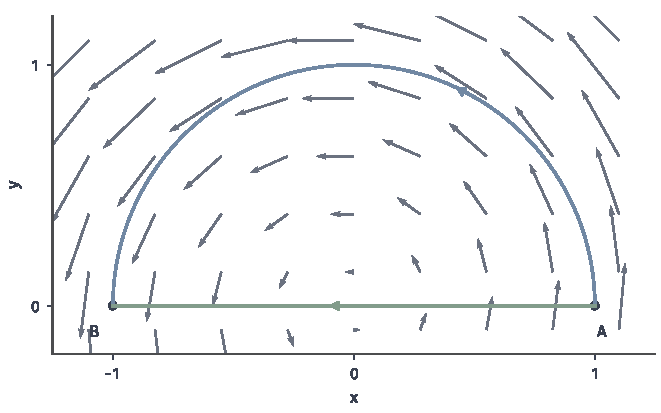
\includegraphics[width=112.0mm]{figures/00-shared/mathematical-preliminaries-upper/00-shared/matplotlib/chapter3-concept-processes/rotation-field-paths.pdf}
 \caption{灰箭头为旋转场$\bm F=(-y,x)^\top$，箭头长度统一缩放为实际场值的$1/4$。两条路径都从$A=(1,0)$到$B=(-1,0)$：蓝色上半圆与场同向，积分为$\pi$；绿色直径上场与位移垂直，积分为零。旋转场处处光滑，端点相同的两条路径上积分仍可不同；下一小节说明势函数给出的路径无关条件。}
 \label{fig:analysis-process-rotation-field-paths}
\end{figure}

\subsection{路径无关与势函数}
\label{sec:multivariable-potential-path-independence}

重力的功只依赖起点和终点的高度，旋转场的功却依赖路线。区别在于：重力的功可以写成某个只依赖位置的量在两端的差，这个量是$-mgy$；旋转场则没有这样的量。
本小节先说明这样的量，即势函数，如何把沿途累计化为端点差；再证明“功与路线无关”反过来也能构造出势函数；最后给出可以直接检查的微分条件，并说明定义域中有洞时，这个条件为什么不再足以保证势函数存在。

\subsubsection{势函数与路径积分}

\paragraph{势函数}

物理中，地面附近质量为$m$的物体在高度$y$处的重力势能为$E_{\mathrm p}(x,y)=mgy$。重力等于势能梯度的相反向量：$-\nabla E_{\mathrm p}=(0,-mg)^\top$。物体下降时势能减少，减少的势能等于重力做的功。
数学中习惯省去负号，取$\phi=-E_{\mathrm p}$，直接要求向量场等于某个标量函数的梯度。
\begin{definition}[势函数]
设$U\subseteq\mathbb R^d$为非空开集，$\bm F:U\to\mathbb R^d$连续。
若存在$\phi\in C^1(U)$使$\bm F=\nabla\phi$，称$\phi$为$\bm F$的\term{势函数}（potential function），称$\bm F$为梯度场，也称保守场。
\end{definition}

梯度指向函数增长最快的方向，所以在梯度非零处，梯度场的箭头指向$\phi$增大的方向，也就是势能$-\phi$减小的方向：重力把物体拉向低处。
例如$\phi(x,y)=x^2+y^2$给出$\bm F(x,y)=(2x,2y)^\top$，箭头从原点向外，因为离原点越远$\phi$越大；常场$(1,0)^\top$的一个势函数是$\phi(x,y)=x$。

给势函数加一个常数，梯度不变，所以势函数不唯一。若$U$还是路径连通的，两个势函数也只能相差一个常数：它们之差的梯度处处为零，路径连通的开集中任意两点都能用域内折线连接，沿折线逐段使用中值公式（定理~\ref{thm:multivariable-scalar-mean-value}），可知这个差在任意两点取值相同。
这与物理中势能的零点可以任选是同一件事：把地面还是桌面取作高度零点，算出的势能差都一样。

“保守”这个名称来自能量守恒。

设质量为$m$的质点在力场$\bm F=\nabla\phi$中按牛顿第二定律$m\gamma''(t)=\bm F(\gamma(t))$运动，其中$\gamma$为$C^2$路径。依次用乘积法则、运动方程和链式法则，得到
\[
 \frac{\mathrm d}{\mathrm dt}\Bigl(\tfrac12m\lVert\gamma'(t)\rVert_2^2\Bigr)
 =m\gamma''(t)^\top\gamma'(t)=\nabla\phi(\gamma(t))^\top\gamma'(t)
 =\frac{\mathrm d}{\mathrm dt}\phi(\gamma(t)),
\]
所以动能与势能$-\phi$之和$\frac12m\lVert\gamma'\rVert_2^2-\phi(\gamma)$的导数为零，不随时间变化。最后一个等号已经显示了下面定理的核心：沿路径的功率$\nabla\phi^\top\gamma'$恰是$\phi\circ\gamma$的导数。

\paragraph{路径积分基本定理}

一元基本定理说，导数在区间上的积分等于原函数在两端的差。把势函数与路径复合，得到一元函数$t\mapsto\phi(\gamma(t))$，它的导数恰是第二类路径积分的被积函数，因此一元基本定理直接给出端点差。
直观上，每一小段的功$\nabla\phi^\top\Delta\bm r$近似等于$\phi$在这一小段上的增量，这些增量相加时中间各项逐一抵消，只剩终点值减起点值。
\begin{theorem}[路径积分基本定理]
设$U\subseteq\mathbb R^d$为开集，$\phi\in C^1(U)$，$\gamma:[a,b]\to U$分段$C^1$。则
\begin{equation}
  \int_{\gamma}\nabla\phi\mathbin{\cdot}\mathrm{d}\bm{r}
  =\phi(\gamma(b))-\phi(\gamma(a)).
\label{eq:analysis-line-integral-gradient}
\end{equation}
\end{theorem}
\begin{proof}
在每个光滑参数段$[t_{j-1},t_j]$上，链式法则给出
\[
 (\phi\circ\gamma)'(t)=\nabla\phi(\gamma(t))^\top\gamma'(t).
\]
右侧是连续函数的复合与乘积，在该段上连续，所以对该段使用一元基本定理，得到
$\int_{t_{j-1}}^{t_j}\nabla\phi(\gamma(t))^\top\gamma'(t)\,\mathrm dt=\phi(\gamma(t_j))-\phi(\gamma(t_{j-1}))$。
对$j=1,\dots,n$相加，中间端点的值一正一负逐一抵消，只剩$\phi(\gamma(b))-\phi(\gamma(a))$。
\end{proof}

用势能$E_{\mathrm p}=-\phi$来读，式~\eqref{eq:analysis-line-integral-gradient}说：保守力沿任何路线做的功都等于起点势能减终点势能，即势能的下降量。示例~\ref{ex:analysis-gravity-work}的重力做功就是$\phi(x,y)=-mgy$的情形。

这个定理有两个直接推论。第一，梯度场的积分只依赖端点：两条端点相同的路线，功相同。第二，闭路径的起点与终点重合，所以梯度场沿任意闭路径的积分为零：把书从地上拿到桌上再放回地上，重力在全过程中做的总功为零。
方向反转时端点交换，端点差变号，这与第二类积分的方向反转性质一致。

知道势函数后，计算路径积分不必代入参数。
\begin{example}[用势函数计算沿半圆的积分]
取$\bm F=(2x,2y)^\top$，它的势函数为$\phi(x,y)=x^2+y^2$。路径取示例~\ref{ex:analysis-path-integral-comparison}中的上半圆$\gamma(t)=(\cos t,\sin t)^\top$，$0\leq t\leq\pi$，从$(1,0)$走到$(-1,0)$。由式~\eqref{eq:analysis-line-integral-gradient}，
\[
 \int_\gamma\bm F\cdot\mathrm d\bm r=\phi(-1,0)-\phi(1,0)=1-1=0.
\]
直接代入参数也得到同样结果：$\bm F(\gamma(t))^\top\gamma'(t)=2\cos t\,(-\sin t)+2\sin t\cos t=0$。这个场在圆周上处处沿半径方向，与切线垂直。
\end{example}

第二个推论还可以用来否定势函数的存在。旋转场沿单位圆逆时针一周做功$2\pi\neq0$，所以它在$\mathbb R^2$上没有势函数。

\subsubsection{路径无关的等价判别}

\paragraph{路径无关}

路径积分基本定理说明，有势函数就能推出功与路线无关。要讨论反方向，先把“与路线无关”说准确。比较同一对端点间的不同路线，需要域内任意两点都能用路径连接；对欧氏开集，路径连通时任意两点之间还能选到域内的折线，因而能选到分段光滑路径。
\begin{definition}[路径无关]
设$U\subseteq\mathbb R^d$为非空、开且路径连通的集合，$\bm F:U\to\mathbb R^d$连续。
若对任意$\bm a,\bm b\in U$及域内从$\bm a$到$\bm b$的任意两条分段$C^1$路径，第二类路径积分都相等，称$\bm F$的路径积分与路径无关。
\end{definition}

反方向的想法来自物理中定义势能的办法：选定一个参考点作为势能零点，把力从参考点到某点所做的功取负号，作为该点的势能。只有当这个功与所选路线无关时，这样定义的势能才是一个确定的数。下面的定理说明，路径无关、闭路径积分为零与势函数存在三者等价。
\begin{theorem}[路径无关的等价条件]
设$U\subseteq\mathbb R^d$非空、开且路径连通，$\bm F:U\to\mathbb R^d$连续。下列条件等价：
\begin{enumerate}
 \item 存在$\phi\in C^1(U)$使$\nabla\phi=\bm F$；
 \item $\bm F$的路径积分与路径无关；
 \item 域内每条分段$C^1$闭路径的积分都为零。
\end{enumerate}
\end{theorem}
\begin{proof}
条件1推出条件2，是路径积分基本定理的第一个推论。
条件2推出条件3：设$\gamma$是从$\bm a$出发回到$\bm a$的闭路径。停在$\bm a$不动的常值路径也从$\bm a$到$\bm a$，它的速度为零，积分为零；由路径无关，$\gamma$上的积分也为零。
条件3推出条件2：设$\gamma_1,\gamma_2$都从$\bm a$到$\bm b$。先沿$\gamma_1$走到$\bm b$，再沿$\gamma_2$的反向路径$\gamma_2^-$走回$\bm a$，拼成闭路径$\gamma_1*\gamma_2^-$。由拼接和方向反转性质，
\[
 0=\int_{\gamma_1*\gamma_2^-}\bm F\cdot\mathrm d\bm r
 =\int_{\gamma_1}\bm F\cdot\mathrm d\bm r-\int_{\gamma_2}\bm F\cdot\mathrm d\bm r.
\]

最后由条件2构造势函数。固定参考点$\bm a\in U$，对每个$\bm x\in U$，取域内任意一条从$\bm a$到$\bm x$的分段$C^1$路径，令$\phi(\bm x)$为沿它的积分。路径无关保证这个数不依赖所选路线。
下面计算偏导数。因为$U$开，存在$r>0$使以$\bm x$为中心、半径$r$的球在$U$内。对$0<|h|<r$，到$\bm x+h\bm e_j$的一条路径可以这样选：先沿原来的路径走到$\bm x$，再沿第$j$个坐标方向走线段$t\mapsto\bm x+t\bm e_j$，$t$从$0$到$h$。线段的速度为$\bm e_j$，场与速度的内积是第$j$个分量$F_j$，于是
\[
 \phi(\bm x+h\bm e_j)-\phi(\bm x)
 =\int_0^h F_j(\bm x+t\bm e_j)\,\mathrm dt.
\]
（$h<0$时按有向积分理解。）右侧除以$h$，是$F_j$在这条短线段上的平均值。$F_j$连续，$h\to0$时这个平均值趋于$F_j(\bm x)$，所以$\partial_j\phi(\bm x)=F_j(\bm x)$。
所有偏导数都等于$\bm F$的连续分量，故$\phi\in C^1(U)$且$\nabla\phi=\bm F$，得到条件1。
\end{proof}

证明中的$\phi$正是“从参考点出发做的功”。换一个参考点$\bm a'$，$\phi$只改变一个常数，即从$\bm a'$到$\bm a$的功，这与势能零点可以任选一致。

\subsubsection{势函数存在的微分判别}

\paragraph{交叉偏导相等的必要条件}

路径无关的等价条件把势函数的存在归结为检查所有路径或所有闭路径，实际上无法逐条验证。我们希望找到只需对$\bm F$求导就能检查的条件。
若$\bm F=\nabla\phi$，则$F_j=\partial_j\phi$。当$\bm F$本身是$C^1$时，$\phi$具有连续的二阶偏导数，由定理~\ref{thm:multivariable-mixed-partials}，混合偏导可以交换次序，于是$\bm F$的分量之间必须满足一组关系。
\begin{theorem}[保守场的必要条件]
设$U\subseteq\mathbb R^d$为开集，$\bm F\in C^1(U;\mathbb R^d)$。
若$\bm F=\nabla\phi$，其中$\phi\in C^1(U)$，则对所有$i,j$和$\bm x\in U$，有
\[
 \partial_iF_j(\bm x)=\partial_jF_i(\bm x).
\]
\end{theorem}
\begin{proof}
由$\partial_j\phi=F_j\in C^1(U)$可知$\phi\in C^2(U)$，因此
$\partial_iF_j=\partial_i\partial_j\phi=\partial_j\partial_i\phi=\partial_jF_i$。
\end{proof}

在平面中，记$\bm F=(P,Q)^\top$，条件只有一个：$\partial_xQ=\partial_yP$。差$\partial_xQ-\partial_yP$有清楚的几何含义：它度量向量场在一点附近的旋转程度。

为看出这一点，计算沿一个小正方形边界的环流。

设正方形为$[x_0,x_0+\delta]\times[y_0,y_0+\delta]$，按逆时针方向行走。下边向右，贡献$\int_{x_0}^{x_0+\delta}P(x,y_0)\,\mathrm dx$；上边向左，贡献$-\int_{x_0}^{x_0+\delta}P(x,y_0+\delta)\,\mathrm dx$。$P$在上下两边相差约$\partial_yP\,\delta$，所以这两项之和约为$-\partial_yP\cdot\delta\cdot\delta$。同理，右边向上、左边向下，两者的贡献之和约为$\partial_xQ\cdot\delta^2$。
因此小正方形的环流约为$(\partial_xQ-\partial_yP)\,\delta^2$，即单位面积上的环流约为$\partial_xQ-\partial_yP$，下面称它为旋转率。

保守场沿每条闭路径做功为零，小正方形也不例外，所以旋转率必须处处为零，这与上面的必要条件一致。这里只是近似推理；沿区域边界的环流与区域内旋转率的精确关系是Green公式，见定理~\ref{thm:multivariable-green}。

两个例子可以对照。场$(2x,2y)^\top$满足$\partial_xQ=0=\partial_yP$，它确实有势函数$x^2+y^2$。旋转场$(-y,x)^\top$有$\partial_xQ-\partial_yP=1-(-1)=2\neq0$，它在每一点附近都在旋转，由上面的必要条件，它在任何非空开集上都没有势函数。这与单位圆上环流为$2\pi$的计算一致：$2\pi$恰是旋转率$2$乘单位圆盘的面积$\pi$。

\paragraph{星形域上的充分条件}

交叉偏导相等只说明每个小区域内没有旋转，它是局部条件；势函数却要在整个定义域上用一个函数表示。要从局部条件得到全局结论，还需要对定义域本身加条件。

一个便于直接构造的条件是星形：若存在$\bm a\in U$，使从$\bm a$到每个$\bm x\in U$的整条线段都在$U$内，称$U$关于$\bm a$星形。凸开集满足这一条件，整个$\mathbb R^d$也满足。
在星形域上，可以沿用路径无关等价条件证明中“从参考点出发做功”的办法定义势函数，并且总沿直线段从$\bm a$走到$\bm x$。
\begin{theorem}[星形域上势函数的构造]
设$U\subseteq\mathbb R^d$为关于$\bm a$星形的开集，$\bm F\in C^1(U;\mathbb R^d)$，且对所有$i,j$有$\partial_iF_j=\partial_jF_i$。则
\[
 \phi(\bm x)=\int_0^1\bm F(\bm a+t(\bm x-\bm a))^\top(\bm x-\bm a)\,\mathrm dt
\]
属于$C^1(U)$且满足$\nabla\phi=\bm F$。因此$\bm F$的路径积分与路径无关。
\end{theorem}
\begin{proof}
记$\bm z=\bm x-\bm a$。$\phi(\bm x)$是$\bm F$沿线段$t\mapsto\bm a+t\bm z$，$0\leq t\leq1$，的第二类路径积分，因为这条线段的速度恒为$\bm z$。
固定$\bm x$时，这条线段是$U$内的紧集，因而它的一个足够小的紧邻域仍在$U$内；当$\bm x$在一个小范围内变动时，相应线段都留在这个紧邻域中。
$\bm F$及其一阶偏导在紧邻域上连续因而有界，所以被积函数对$x_j$的偏导数有不依赖$t$的上界，可以用式~\eqref{eq:classical-differentiate-under-integral}在积分号下对$x_j$求导。

被积函数为$\sum_iF_i(\bm a+t\bm z)z_i$。对$x_j$求导时，$z_j$对$x_j$的导数为$1$，$F_i(\bm a+t\bm z)$对$x_j$的导数由链式法则为$t\,\partial_jF_i(\bm a+t\bm z)$，所以偏导数为
\[
 F_j(\bm a+t\bm z)+t\sum_i z_i\partial_jF_i(\bm a+t\bm z).
\]
交叉偏导条件把$\partial_jF_i$换成$\partial_iF_j$，而$\sum_iz_i\partial_iF_j(\bm a+t\bm z)$正是$t\mapsto F_j(\bm a+t\bm z)$的导数，于是
\[
 \begin{aligned}
 F_j(\bm a+t\bm z)+t\sum_i z_i\partial_jF_i(\bm a+t\bm z)
 &=F_j(\bm a+t\bm z)+t\sum_i z_i\partial_iF_j(\bm a+t\bm z)\\
 &=\frac{\mathrm d}{\mathrm dt}\bigl[tF_j(\bm a+t\bm z)\bigr].
 \end{aligned}
\]
对$t$从$0$积分到$1$，由一元基本定理得$\partial_j\phi(\bm x)=1\cdot F_j(\bm a+\bm z)-0=F_j(\bm x)$。
这些偏导连续，所以$\phi\in C^1(U)$；路径无关由前一定理得到。
\end{proof}

用这个构造可以求出一个具体平面场的势函数。
\begin{example}[沿线段构造势函数$x^2y$]
取$\bm F(x,y)=(2xy,x^2)^\top$，即$P=2xy$，$Q=x^2$。它定义在整个平面上，分量都是多项式，属于$C^1$，并且$\partial_yP=2x=\partial_xQ$。整个平面关于$\bm a=\bm0$星形，代入构造公式，
\[
 \phi(x,y)=\int_0^1\bigl[2(tx)(ty)\,x+(tx)^2\,y\bigr]\,\mathrm dt
 =\int_0^13t^2x^2y\,\mathrm dt=x^2y.
\]
直接求导可验证$\nabla\phi=(2xy,x^2)^\top$。于是这个场沿任何从$(0,0)$到$(1,2)$的分段$C^1$路径做功都等于$\phi(1,2)-\phi(0,0)=2$。
\end{example}
星形域上的构造不依赖猜测：交叉偏导相等时，沿线段积分就给出势函数，任意路径上的功随之化为端点差。

\paragraph{穿孔平面上的反例}

星形域的条件不能省略。下面的向量场在原点以外处处满足交叉偏导条件，在穿孔平面上却没有势函数。
\begin{example}[穿孔平面上的涡旋场]
\label{ex:analysis-punctured-plane-vortex}
在穿孔平面$\mathbb R^2\setminus\{\bm0\}$上考虑
\[
 \bm F(x,y)=\left(-\frac{y}{x^2+y^2},\frac{x}{x^2+y^2}\right)^\top ,
\]
记它的两个分量为$P,Q$。它与旋转场$(-y,x)^\top$方向相同，都沿逆时针方向与以原点为圆心的圆相切，但大小改为到原点距离的倒数：离原点越近转得越快，类似于绕一根细涡管旋转的水流。原点处它没有定义。

先检查交叉偏导。由商的求导法则，
\[
 \begin{aligned}
 \partial_yP&=-\frac{(x^2+y^2)-y\cdot2y}{(x^2+y^2)^2}=\frac{y^2-x^2}{(x^2+y^2)^2},\\
 \partial_xQ&=\frac{(x^2+y^2)-x\cdot2x}{(x^2+y^2)^2}=\frac{y^2-x^2}{(x^2+y^2)^2},
 \end{aligned}
\]
两者在穿孔平面上处处相等，所以这个场在原点以外的每一点附近都没有旋转。

再沿单位圆$\gamma(t)=(\cos t,\sin t)^\top$，$0\leq t\leq2\pi$，逆时针走一周。在单位圆上$x^2+y^2=1$，$\bm F(\gamma(t))=(-\sin t,\cos t)^\top$与速度相同，内积为$1$，积分为$2\pi$。
闭路径积分不为零，由路径无关的等价条件，$\bm F$在穿孔平面上没有势函数。
\end{example}

交叉偏导相等这个局部条件，在这里没能给出全局的势函数。这与星形域上的定理并不矛盾：穿孔平面不是星形域，对任一点$\bm a\neq\bm0$，从$\bm a$到$-\bm a$的线段都经过原点。问题出在原点这个洞上，可以从两个角度理解。

第一，局部的势函数是极角。在不含原点的区域上，若能连续地选取点$(x,y)$的极角$\theta$，使$x=r\cos\theta$、$y=r\sin\theta$，其中$r=\sqrt{x^2+y^2}$，则直接求导可得$\nabla\theta=\bm F$。例如在右半平面$x>0$上取$\theta=\arctan(y/x)$，有$\partial_x\theta=-y/(x^2+y^2)$，$\partial_y\theta=x/(x^2+y^2)$。
在更大的区域，即去掉负半轴的平面$\mathbb R^2\setminus\{(x,0)^\top:x\leq0\}$上，取$\theta\in(-\pi,\pi)$，它连续且仍满足$\nabla\theta=\bm F$；这个区域关于$(1,0)$星形，与星形域上的定理一致。

但在整个穿孔平面上无法连续地选取极角：从$(1,0)$出发绕原点逆时针一周回到$(1,0)$，极角连续地增加了$2\pi$，起点和终点处的“势函数值”对不上。单位圆上的积分$2\pi$正是极角的这个增量。
具体地，从$(1,0)$到$(-1,0)$，沿上半圆极角从$0$增加到$\pi$，积分为$\pi$；沿下半圆$(\cos t,-\sin t)^\top$，$0\leq t\leq\pi$，极角从$0$减少到$-\pi$，积分为$-\pi$。两条路线的功相差$2\pi$，恰是绕原点一圈的积分。
不绕原点的闭路径则没有这个问题。例如以$(3,0)$为圆心、半径为$1$的圆整个落在右半平面中，那里$\theta$是势函数，沿它的积分为零。

第二，从小正方形的环流看。交叉偏导相等说明每个小正方形的环流近似为零。若一条闭路径围住的区域整个在定义域内，可以把这个区域划分成许多小正方形；相邻正方形的公共边被沿相反方向各走一次，贡献相互抵消，只剩外边界，于是外边界的环流也为零。这一推理的精确形式就是Green公式（定理~\ref{thm:multivariable-green}），它要求向量场在整个被围区域附近都有定义且连续可微。

单位圆围住的圆盘却包含原点，那里$\bm F$没有定义，无法这样填满。场在定义域内的旋转率处处为零；非零环流与被排除的原点有关。对夹在两条绕原点闭路径之间、不含原点的环形区域作同样的划分，可知两条路径上的环流相等；所以绕原点逆时针一周的简单闭路径，积分都是$2\pi$，而围住的区域不含原点的闭路径，积分为零。

相比之下，星形域上不会出现这样的洞：任何闭路径都可以沿线段向中心点$\bm a$连续收缩而不离开定义域。这从几何上解释了，为什么在星形域上交叉偏导条件已经足以保证势函数存在。

\FloatBarrier

\par\Needspace{10\baselineskip}
\section{曲面积分}
\label{sec:analysis-surface-integration}

路径积分沿一条细线累计：线密度乘弧长得到质量，力与位移的内积累加得到做功。
曲面积分把累计的范围从细线换成薄片，典型问题有两个。
第一个问题是求一张金属薄壳的质量：已知壳上每点每平方米有多少千克，把各小片的“面密度乘面积”加起来即可。
第二个问题是求单位时间内有多少水穿过一张渔网：水在各点有速度，只有垂直于网面的速度分量才把水送到网的另一侧。

两个问题的被积对象不同。
在第一个问题中，被积对象是曲面$S$上的标量函数$h:S\to\mathbb R$，它给出每单位面积的密度，乘面积后相加得到质量、电荷等总量。
在第二个问题中，被积对象是向量场$\bm F:S\to\mathbb R^3$，它在每点给出一个有大小和方向的量；要先取它垂直于曲面的分量，再乘面积相加，得到穿过曲面的\emph{通量}。

两类积分都需要知道曲面上一小片有多大，所以本节先用参数化求出面积元。
通量还需要规定“从哪一侧穿到哪一侧算正”，因此在定义第二类积分之前，还要讨论曲面的定向。
本节的参数积分都按有界Jordan区域上的Riemann积分理解；参数曲面、面积元和通量的标准构造可参考\scite{math-openstax-calculus3}。

\subsection{参数曲面与面积元}

平面区域的面积就是它的Jordan面积。
空间中的曲面一般是弯曲的，不能不经伸缩地摊平成平面区域，所以不能直接用参数域的面积计算它的面积。
处理地球表面时，人们用经度和纬度两个数确定地面上的一点，这就是一种参数化：用两个参数标记曲面上的点，把曲面上的累计转回二维参数域上计算。
代价是参数域中的面积一般不等于曲面上的实际面积。
经纬度网格上同样大小的格子，在赤道附近和两极附近对应的实际地面面积并不相同，因此每一点都要乘一个面积放大倍数来校正。
本小节先说明怎样的参数化才能描述一张面，再求出这个放大倍数，并证明由此得到的面积不依赖参数的选取。

\subsubsection{曲面的参数化}

\paragraph{正则曲面片}

曲面的参数化是一个向量值映射：输入两个实数$(u,v)$，输出空间中一点的三个坐标。
并不是每个这样的映射都描述一张面。
若改变两个参数时点只沿同一个方向移动，像集可能只是一条曲线；
若不同参数在一块正面积的范围内对应同一些点，按参数累计就会把这块面计算两次。
下面的定义用正则性和单次覆盖两个条件分别排除这两种情况。

\begin{definition}[正则参数曲面片]
\label{def:analysis-regular-surface-patch}
设$E\subseteq\mathbb R^2$是有界闭区域，$E=\overline{E^\circ}$，其边界$\partial E$可用总面积任意小的有限个矩形覆盖。
设$\bm r$在$E$的一个开邻域内是$C^1$映射，写成
\[
 \bm r(u,v)=(x(u,v),y(u,v),z(u,v))^\top\in\mathbb R^3.
\]
若不同参数只有在都属于$\partial E$时才允许表示同一点，
且两个偏导向量$\bm r_u,\bm r_v$在$E^\circ$上处处线性无关，则称$\bm r$为一个正则曲面片的参数化，曲面片记为$S=\bm r(E)$。
参数边界允许产生接缝或退化点；这些边界部分按零曲面面积处理。
\end{definition}

定义中的两个偏导向量有直接的几何含义。
固定$v$而只改变$u$，点$\bm r(u,v)$在曲面上画出一条参数曲线，它的速度向量是$\bm r_u$；
固定$u$而改变$v$得到另一条参数曲线，速度向量是$\bm r_v$。
这里$\bm r_u,\bm r_v$都是三维向量，分别由三个坐标函数对同一个参数求偏导得到，并非某个标量函数的两个偏导数。

两个向量线性无关，是指对任意实数$\alpha,\beta$，
$\alpha\bm r_u+\beta\bm r_v=\bm0$只有在$\alpha=\beta=0$时才成立。
几何上，这表示两个向量不共线，它们张成过该点的一个平面，即曲面的切平面。
若这个条件不成立，像集可能根本不是一张面。

\begin{example}[像集退化为线段的参数映射]
取$E=[0,1]^2$和$\bm r(u,v)=(u+v,0,0)^\top$。
两个偏导向量都等于$(1,0,0)^\top$，因而线性相关。
当$(u,v)$取遍$E$时，$u+v$取遍$[0,2]$，所以像集是$x$轴上的线段$\{(x,0,0)^\top:0\leq x\leq2\}$。
整个正方形被压到这条线段上，像集上没有两个不共线的切方向，也没有面积可言；这个映射不满足正则性条件。
\end{example}

正则性条件排除了这种压扁的映射。
单次覆盖条件处理另一种情况：像集确实是一张面，但被参数重复计数。

\begin{example}[圆柱面的单次覆盖与二重覆盖]
\label{ex:analysis-cylinder-double-cover}
高为$1$的单位圆柱面可以写成
\[
\begin{gathered}
\bm r(\theta,z)=(\cos\theta,\sin\theta,z)^\top\\
z\in[0,1].
\end{gathered}
\]
偏导向量$\bm r_\theta=(-\sin\theta,\cos\theta,0)^\top$与$\bm r_z=(0,0,1)^\top$处处线性无关，正则性没有问题，需要检查的只有覆盖次数。
若$\theta\in[0,2\pi]$，只有$\theta=0$与$\theta=2\pi$两条边界线表示同一条接缝，这是定义允许的。
若$\theta\in[0,4\pi]$，则对$0<\theta_0<2\pi$和$0<z<1$，点$\bm r(\theta_0,z)$同时由参数域内部的$(\theta_0,z)$和$(\theta_0+2\pi,z)$表示；
按参数累计会把整张柱面计入两次，因此这一参数域不符合定义。
\end{example}

所以不同参数表示同一点的情形只允许出现在参数边界上，形成接缝；参数域内部的点不能与任何其他参数点表示同一点。

本小节反复使用的例子是$\bm r(u,v)=(u,v,u+v)^\top$、$E=[0,1]^2$，下文称它为斜平面片。
它描述平面$z=x+y$上位于单位正方形上方的一块平行四边形，
两个切向量分别为$\bm r_u=(1,0,1)^\top$和$\bm r_v=(0,1,1)^\top$。
前两个坐标就是参数本身，所以不同参数给出不同点；两个切向量不共线，所以它满足正则曲面片的定义。

\paragraph{叉积}

要求曲面的面积，先看参数域中的一个小矩形$[u,u+\Delta u]\times[v,v+\Delta v]$被映成什么形状。
由$\bm r$的可微性，在$\Delta u,\Delta v$很小时有线性近似
\[
 \bm r(u+\Delta u,v+\Delta v)\approx\bm r(u,v)+\bm r_u\Delta u+\bm r_v\Delta v,
\]
其中$\bm r,\bm r_u,\bm r_v$都在$(u,v)$处取值。
于是小矩形的四个顶点近似映为
$\bm r$、$\bm r+\bm r_u\Delta u$、$\bm r+\bm r_v\Delta v$和$\bm r+\bm r_u\Delta u+\bm r_v\Delta v$，
它们正是以$\bm r_u\Delta u$和$\bm r_v\Delta v$为两边的平行四边形的顶点。
所以曲面上的小片近似是切平面内的一个小平行四边形，问题归结为：怎样由两条边向量求平行四边形的面积。

在平面上，两个边向量排成$2\times2$矩阵，其行列式的绝对值就是这个面积。
现在两条边是三维向量，排成的是$3\times2$矩阵，没有行列式可取。
三维空间中常用叉积同时记录这个面积和平行四边形所在平面的垂直方向。
对$\bm a,\bm b\in\mathbb R^3$，定义叉积
\[
 \bm a\times\bm b
 =(a_2b_3-a_3b_2,\ a_3b_1-a_1b_3,\ a_1b_2-a_2b_1)^\top.
\]
例如$(1,0,0)^\top\times(0,1,0)^\top=(0,0,1)^\top$：
$x$轴方向与$y$轴方向的单位向量张成面积为$1$的正方形，叉积是长度为$1$、沿$z$轴的向量。

后面的面积和法向计算要用到叉积的三条性质，下面逐一核对。
第一，叉积垂直于$\bm a$和$\bm b$。直接展开
\[
 \bm a^\top(\bm a\times\bm b)
 =a_1(a_2b_3-a_3b_2)+a_2(a_3b_1-a_1b_3)+a_3(a_1b_2-a_2b_1),
\]
右端六项两两抵消，结果为$0$；对$\bm b$同理。
垂直于同一平面的方向有相反的两个，叉积按右手规则选取其中之一：右手四指从$\bm a$弯向$\bm b$时，拇指指向$\bm a\times\bm b$。

第二，叉积的长度等于$\bm a,\bm b$张成的平行四边形的面积。
把两边按分量展开，可以验证Lagrange恒等式
\[
 \lVert\bm a\times\bm b\rVert_2^2
 =\lVert\bm a\rVert_2^2\lVert\bm b\rVert_2^2-(\bm a^\top\bm b)^2.
\]
记$\theta\in[0,\pi]$为两向量的夹角，则$\bm a^\top\bm b=\lVert\bm a\rVert_2\lVert\bm b\rVert_2\cos\theta$，
代入得$\lVert\bm a\times\bm b\rVert_2=\lVert\bm a\rVert_2\lVert\bm b\rVert_2\sin\theta$。
以$\bm a$为底边时，平行四边形的高是$\lVert\bm b\rVert_2\sin\theta$，所以叉积长度正是“底乘高”。
特别地，叉积为零当且仅当两向量线性相关，即平行四边形退化为线段或一点。

第三，叉积对每个因子都是线性的，交换两个因子的次序会变号：从定义式直接看出$\bm b\times\bm a=-\bm a\times\bm b$，特别地$\bm a\times\bm a=\bm0$。
这与右手规则一致：交换次序后四指的弯曲方向相反，拇指也随之反向。

把这些性质用到小平行四边形上。由线性，
$(\bm r_u\Delta u)\times(\bm r_v\Delta v)=(\bm r_u\times\bm r_v)\Delta u\Delta v$；
再由第二条性质，小曲面片的面积近似为
\[
 \lVert\bm r_u\times\bm r_v\rVert_2\,\Delta u\,\Delta v.
\]
因此$\lVert\bm r_u\times\bm r_v\rVert_2$就是参数化在该点的面积放大倍数：参数域中面积为$\Delta u\Delta v$的小块，
在曲面上变成面积约为这个倍数乘$\Delta u\Delta v$的小片。
同样由第二条性质，正则性条件“两个切向量线性无关”可以等价地写成$\bm r_u\times\bm r_v\ne\bm0$，即放大倍数处处为正。

平面情形可以用来核对这个倍数。若曲面就在平面$z=0$内，即$\bm r(u,v)=(x(u,v),y(u,v),0)^\top$，
则$\bm r_u\times\bm r_v=(0,0,x_uy_v-x_vy_u)^\top$，其长度正是映射$(u,v)\mapsto(x,y)$的Jacobian行列式的绝对值。
这与第~\ref{sec:classical-change-variables}节换元公式中的面积权重$|\det\bm J_T|$一致；叉积长度是这个权重在三维空间中的推广。

\subsubsection{曲面面积的表示}

\paragraph{面积元与面积}

把参数域分成许多小矩形，由小平行四边形的面积近似，每块在曲面上的像的面积约为放大倍数乘参数面积，曲面的总面积约为这些乘积之和。
小矩形越细，线性近似越准确，求和的极限就是放大倍数在参数域上的积分。

这里直接把这个积分取作曲面面积的定义，而不像弧长那样用内接折线长度的上确界来定义，因为曲面上的类似做法会失败。
在一段有限高的圆柱面上，可以构造顶点都在柱面上的三角形网格（称为Schwarz灯笼），
使网格越来越细，三角形与柱面的夹角却不趋于零，三角形总面积可以趋于无穷。
用切平面上的平行四边形近似则不会出现这种问题，因为每个小平行四边形都贴着切平面。

\begin{definition}[曲面面积]
\label{def:analysis-surface-area-measure}
在单次覆盖的正则曲面片上，令$J_S=\|\bm r_u\times\bm r_v\|_2$。定义面积为
\[
 \operatorname{area}(S)=\iint_E J_S(u,v)\,\mathrm du\,\mathrm dv.
\]
面积元记为$\mathrm dS=J_S(u,v)\,\mathrm du\,\mathrm dv$。
\end{definition}

$J_S$在紧参数域上连续，所以积分存在。有限分片曲面的面积逐片相加；各片只沿边界接合，接缝的参数原像须能被任意小总面积的有限盒覆盖，以免重复累计。

用这一定义计算斜平面片的面积，并用初等几何核对结果。

\begin{example}[斜平面片的面积]
\label{ex:analysis-tilted-plane-area}
对斜平面片$\bm r(u,v)=(u,v,u+v)^\top$、$E=[0,1]^2$，按叉积的定义计算
\[
 \begin{aligned}
 \bm r_u\times\bm r_v
 &=(1,0,1)^\top\times(0,1,1)^\top\\
 &=(0\cdot1-1\cdot1,\ 1\cdot0-1\cdot1,\ 1\cdot1-0\cdot0)^\top
 =(-1,-1,1)^\top,
 \end{aligned}
\]
故$J_S=\lVert(-1,-1,1)^\top\rVert_2=\sqrt3$处处成立，曲面面积为
\[
 \operatorname{area}(S)=\int_0^1\int_0^1\sqrt3\,\mathrm du\,\mathrm dv=\sqrt3.
\]
用初等几何核对：两条边$\bm r_u,\bm r_v$的长度都是$\sqrt2$，内积为$1$，夹角余弦为$1/2$，即夹角为$60^\circ$；
平行四边形面积为$\sqrt2\cdot\sqrt2\cdot\sin60^\circ=\sqrt3$，与积分结果相同。
\end{example}

参数正方形的面积只有$1$，曲面片的面积却是$\sqrt3$：每个参数小块都被放大$\sqrt3$倍。
图~\ref{fig:analysis-process-surface-area-stretch}将参数小块与实际斜面小块对应起来，显示叉积长度校正的是哪一个面积。
\begin{figure*}[!htbp]
 \centering
 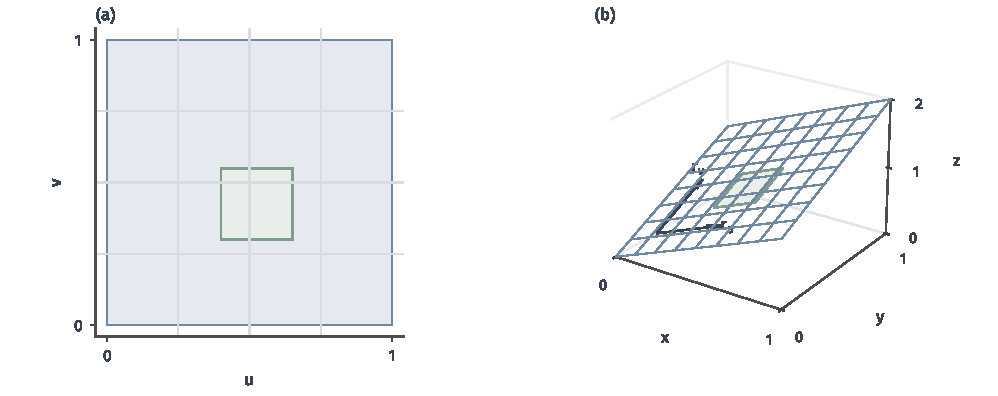
\includegraphics[width=169.0mm]{figures/00-shared/mathematical-preliminaries-upper/00-shared/matplotlib/chapter3-concept-processes/surface-area-stretch.pdf}
 \caption{参数化$r(u,v)=(u,v,u+v)^\top$把单位正方形映为斜平面片，绿色块为同一参数子区间及其像。两切向量$r_u=(1,0,1)^\top$、$r_v=(0,1,1)^\top$在右侧按$0.4$倍画出，叉积长度为$\sqrt3$。每个参数面积都放大$\sqrt3$倍，故不能把$\mathrm du\,\mathrm dv$直接当成$\mathrm dS$。}
 \label{fig:analysis-process-surface-area-stretch}
\end{figure*}

\paragraph{重参数化}

同一张面可以用不同参数标记。
面积是曲面本身的属性，不应随标记方式改变；先在斜平面片上核对一次具体的换参数。

\begin{example}[拉伸一个参数不改变面积]
\label{ex:analysis-stretched-parameter-area}
在斜平面片中令$u=2\xi$，则
\[
\begin{gathered}
\widetilde{\bm r}(\xi,v)=(2\xi,v,2\xi+v)^\top\\
(\xi,v)\in[0,1/2]\times[0,1]
\end{gathered}
\]
描述同一块平行四边形，新参数域的面积只有$1/2$。
另一方面，$\widetilde{\bm r}_\xi=(2,0,2)^\top=2\bm r_u$，$\widetilde{\bm r}_v=\bm r_v$，由叉积的线性，
$\widetilde{\bm r}_\xi\times\widetilde{\bm r}_v=2(\bm r_u\times\bm r_v)=2(-1,-1,1)^\top$，放大倍数为$2\sqrt3$。
因此
\[
 \int_0^1\int_0^{1/2}2\sqrt3\,\mathrm d\xi\,\mathrm dv=\sqrt3,
\]
与示例~\ref{ex:analysis-tilted-plane-area}的结果相同。
\end{example}

参数域缩小一半，每点的放大倍数恰好加倍，两者相互抵消。
下面的定理说明，这种抵消对一般的单次覆盖换参数都成立。

\begin{theorem}[重参数化下的面积元]
\label{thm:analysis-surface-reparameterization}
设$\bm r:E\to S$是正则曲面片的参数化，$T:\widetilde E\to E$是参数域之间的双射，
在$\widetilde E$的一个开邻域内为$C^1$映射，并且限制在$\widetilde E^\circ$上是到$E^\circ$的$C^1$微分同胚。
若$\widetilde{\bm r}=\bm r\circ T$仍满足曲面片条件，则
\[
 \begin{aligned}
 \widetilde{\bm r}_\xi\times\widetilde{\bm r}_\eta
 &=\det\bm J_T\,(\bm r_u\times\bm r_v)\circ T,\\
 \widetilde J_S&=(J_S\circ T)|\det\bm J_T|.
 \end{aligned}
\]
两组参数由此给出同一面积。
\end{theorem}

\begin{proof}
记$T(\xi,\eta)=(u(\xi,\eta),v(\xi,\eta))$。
链式法则给出$\widetilde{\bm r}_\xi=\bm r_u u_\xi+\bm r_v v_\xi$和
$\widetilde{\bm r}_\eta=\bm r_u u_\eta+\bm r_v v_\eta$，其中右端各量在$T(\xi,\eta)$处取值。
用叉积对每个因子的线性展开，得到四项：
\[
 \begin{aligned}
 \widetilde{\bm r}_\xi\times\widetilde{\bm r}_\eta
 &=u_\xi u_\eta(\bm r_u\times\bm r_u)+u_\xi v_\eta(\bm r_u\times\bm r_v)\\
 &\quad{}+v_\xi u_\eta(\bm r_v\times\bm r_u)\\
 &\quad{}+v_\xi v_\eta(\bm r_v\times\bm r_v).
 \end{aligned}
\]
由$\bm a\times\bm a=\bm0$，第一、四项为零；交换叉积次序会变号，即$\bm r_v\times\bm r_u=-\bm r_u\times\bm r_v$，于是第三项可与第二项合并。因此
\[
 \widetilde{\bm r}_\xi\times\widetilde{\bm r}_\eta
 =(u_\xi v_\eta-v_\xi u_\eta)(\bm r_u\times\bm r_v)\circ T,
\]
括号内正是$\det\bm J_T$，这就是第一式；两边取长度得到第二式。
把第二式在新参数域上积分，并应用经典二维换元公式，得到
\[
 \iint_{\widetilde E}(J_S\circ T)|\det DT|
 =\iint_E J_S.
\]
若换元只在参数域内部正则，先在远离边界的紧子域上应用公式，再利用连续有界权重和Jordan边界条件取极限。两组参数因而给出相同面积。
\end{proof}

几何上，这个证明把两步面积放大接在一起：新参数的小方块先由$T$映成原参数域中面积约为$|\det\bm J_T|$倍的小块，
这个小块再由$\bm r$映到曲面，面积又乘$J_S$。
二维换元公式恰好把第一步的倍数吸收掉，所以只剩下曲面本身的面积。
在示例~\ref{ex:analysis-stretched-parameter-area}中，$T(\xi,v)=(2\xi,v)$，$\det\bm J_T=2$，这正是放大倍数加倍的来源。

行列式的绝对值保证面积非负；行列式本身的符号则记录参数次序是否翻转。
例如在斜平面片上交换两个参数，令$T(\xi,\eta)=(\eta,\xi)$，即$\widetilde{\bm r}(\xi,\eta)=\bm r(\eta,\xi)=(\eta,\xi,\xi+\eta)^\top$，则$\det\bm J_T=-1$，
叉积由$(-1,-1,1)^\top$变为$(1,1,-1)^\top$，长度不变而方向相反。
面积不使用这个方向，后面选取通量的法向时则要用到它。

定理还要求$T$是双射。若参数在正面积的范围内重复覆盖，参数积分就会重复累计。
示例~\ref{ex:analysis-cylinder-double-cover}中，$\bm r_\theta\times\bm r_z=(\cos\theta,\sin\theta,0)^\top$，$J_S=1$；
$\theta\in[0,2\pi]$时参数积分给出柱面面积$2\pi$，$\theta\in[0,4\pi]$时却给出$4\pi$，不能当作单次覆盖的曲面面积。

\paragraph{分片曲面}

有些曲面不能用一张正则曲面片描述。单位立方体的表面由六个正方形组成，棱上没有切平面。
球面虽然可以用一张球坐标参数片覆盖（两极位于参数边界上，切向量在那里退化），也常分成上下两个半球分别处理。
本节只处理有限分片的情形：把曲面写成有限张正则曲面片的并，各片内部不重叠，交接部分在相邻曲面片中面积均为零，
整个曲面的面积由各片的面积相加。

例如立方体表面的面积就是六个单位正方形的面积之和$6$，十二条棱的面积为零，不需要在接缝上另加一项。
后面的两类曲面积分同样可以逐片计算再相加。
无界曲面，或不能这样由有限张正则曲面片覆盖的曲面，还需另外处理覆盖和可积性条件。

\subsection{第一类曲面积分}

有了面积，就可以回到本节开头的第一个问题：在曲面上累计一个标量密度。
这类积分只用到小片的面积，不涉及方向。

\subsubsection{积分的定义和可积性}

\paragraph{按面积的积分}

设一张薄金属壳占据曲面$S$，在点$\bm x$附近每单位面积的质量为$h(\bm x)$（单位如千克每平方米）。
把壳分成许多小片$S_j$，在每片内取一点$\bm x_j$。
若每片很小，片内面密度近似为常数$h(\bm x_j)$，这一片的质量约为$h(\bm x_j)\,\operatorname{area}(S_j)$。
把各片质量相加，再让分割越来越细，就得到面密度对面积的积分。
带电薄壳上的电荷量、涂层表面的涂料用量都是同一种累计。
下面将连续密度与面积权重相乘，再在参数域上积分。

\begin{definition}[第一类曲面积分]
\label{def:analysis-scalar-surface-integral}
设$h$是$S$上的连续标量函数，定义它的\term{第一类曲面积分}（scalar surface integral）为
\begin{equation}
 \int_Sh\,\mathrm dS
 =\iint_Eh(\bm r(u,v))J_S(u,v)\,\mathrm du\,\mathrm dv.
 \label{eq:analysis-scalar-surface-integral}
\end{equation}
右侧被积函数连续，因而积分存在且有限。
\end{definition}

式~\eqref{eq:analysis-scalar-surface-integral}右端的计算顺序是：用参数找到曲面上的点，读出该点的密度，乘该点的面积放大倍数，再在参数域上积分。
对定理~\ref{thm:analysis-surface-reparameterization}中的重参数化，把$h\circ\bm r$一并代入换元公式，可见积分值不变。
取$h=1$得到面积，取非负面密度得到质量。
例如在斜平面片上，常数密度$h=2$给出
\[
 \int_S2\,\mathrm dS=\int_0^1\int_0^1 2\sqrt3\,\mathrm du\,\mathrm dv=2\sqrt3,
\]
即面积为$\sqrt3$、每单位面积重$2$的薄片，总质量为$2\sqrt3$。

除了总量，第一类积分还给出曲面上的平均值。

设$0<\operatorname{area}(S)<\infty$且$h$曲面可积，则
\[
 \frac1{\operatorname{area}(S)}\int_Sh\,\mathrm dS
\]
是$h$按面积加权的平均。若$h$表示地球表面各点的气温，这个量就是全球表面平均气温：
每块地面按其实际面积参与平均，而不是按经纬度网格的格子数参与平均。

质量和平均值都只依赖每小片的大小，不依赖从哪一侧看曲面，所以把曲面的朝向反过来，第一类积分不变。

积分继承参数区域积分的线性、单调性和绝对值估计。有限分片上逐片求和，公共接缝不另计面积。特别地，连续密度满足
\[
 \left|\int_S h\,\mathrm dS\right|\leq\sup_S|h|\operatorname{area}(S).
\]
这些性质只依赖面积权重非负，因此改变曲面法向不会改变第一类积分。

\subsubsection{积分的计算}

计算第一类曲面积分分三步：选一个单次覆盖的正则参数化，把$h$与参数化复合，再乘叉积的长度后在参数域上积分。
最常见的两种参数化是函数图像和球坐标。

若曲面是函数$z=\psi(x,y)$在区域$D$上的图像，其中$D$满足定义~\ref{def:analysis-regular-surface-patch}对参数域的要求，$\psi$在$D$的开邻域内为$C^1$，就可以取
$\bm r(x,y)=(x,y,\psi(x,y))^\top$。此时$\bm r_x=(1,0,\psi_x)^\top$、$\bm r_y=(0,1,\psi_y)^\top$，按叉积公式计算得
\[
 \begin{aligned}
 \bm r_x\times\bm r_y
 &=(0\cdot\psi_y-\psi_x\cdot1,\ \psi_x\cdot0-1\cdot\psi_y,\ 1\cdot1-0\cdot0)^\top\\
 &=(-\psi_x,-\psi_y,1)^\top.
 \end{aligned}
\]
叉积的第三分量恒为$1$，所以图像参数化处处正则；前两个坐标就是参数本身，所以单次覆盖也自动成立。
于是对曲面可积的$h$有
\[
 \int_Sh\,\mathrm dS
 =\iint_Dh(x,y,\psi(x,y))\sqrt{1+\psi_x^2+\psi_y^2}\,\mathrm dx\,\mathrm dy.
\]

根号的几何意义如下。记$\gamma$为法向$(-\psi_x,-\psi_y,1)^\top$与$z$轴的夹角，
则$\cos\gamma=1/\sqrt{1+\psi_x^2+\psi_y^2}$。
一块与水平面成角$\gamma$的小平面片，竖直投影到$xy$平面上时面积缩小为原来的$\cos\gamma$倍；
反过来，由投影面积$\mathrm dx\,\mathrm dy$恢复实际面积，就要除以$\cos\gamma$，即乘上这个根号。
曲面越陡，根号越大。例如$z=ax+by+c$在单位圆盘上方的部分，根号处处等于$\sqrt{1+a^2+b^2}$，面积为
$\pi\sqrt{1+a^2+b^2}$；$a=b=0$时它就是水平圆盘的面积$\pi$。
若曲面不能单值地投影到同一坐标平面，例如整张球面在每个$(x,y)$上方有两点，则需换参数化或分片。

半径$R>0$的球面可以取参数
\[
 \begin{gathered}
 \bm r(\varphi,\theta)
 =(R\sin\varphi\cos\theta,R\sin\varphi\sin\theta,R\cos\varphi)^\top,\\
 0\leq\varphi\leq\pi,\quad 0\leq\theta\leq2\pi,
 \end{gathered}
\]
其中$\varphi$是与北极方向的夹角，$\theta$是绕$z$轴转过的角度。求偏导得
\[
 \begin{aligned}
 \bm r_\varphi&=(R\cos\varphi\cos\theta,R\cos\varphi\sin\theta,-R\sin\varphi)^\top,\\
 \bm r_\theta&=(-R\sin\varphi\sin\theta,R\sin\varphi\cos\theta,0)^\top.
 \end{aligned}
\]
这两个向量的内积为零，长度分别为$R$和$R\sin\varphi$；由叉积长度公式（夹角为$\pi/2$），叉积长度为$R^2\sin\varphi$。
这个结果也可以直接看出：$\varphi$增加$\Delta\varphi$时，点沿经线走过约$R\Delta\varphi$；
$\theta$增加$\Delta\theta$时，点沿半径为$R\sin\varphi$的纬线圈走过约$R\sin\varphi\,\Delta\theta$。
小片近似为以这两个长度为边的矩形。靠近两极时纬线圈变小，同样的$\Delta\theta$对应的面积也变小。

在参数域内部$0<\varphi<\pi$、$0<\theta<2\pi$上$\sin\varphi>0$，参数化正则且单次覆盖；
两极与经线接缝来自参数边界，面积为零，不需要单独处理。
先用这个参数化求球面面积。

\begin{example}[球面的面积]
\label{ex:analysis-sphere-area}
对半径为$R$的球面，球坐标参数的面积放大倍数为$J_S=R^2\sin\varphi$，被积函数连续，可以逐次积分：
\[
 \operatorname{area}(S)
 =\int_0^{2\pi}\int_0^\pi R^2\sin\varphi\,\mathrm d\varphi\,\mathrm d\theta
 =2\pi R^2\bigl[-\cos\varphi\bigr]_0^\pi
 =4\pi R^2.
\]
\end{example}





面积权重在求平均时同样不可缺少，下面以上半球面上的平均高度为例。

\begin{example}[上半球面的平均高度]
\label{ex:analysis-hemisphere-average-height}
取上半球面$0\leq\varphi\leq\pi/2$，高度函数$h(\bm x)=z$。
由$J_S=R^2\sin\varphi$，上半球面面积为$2\pi R^2\int_0^{\pi/2}\sin\varphi\,\mathrm d\varphi=2\pi R^2$，而
\[
 \int_Sz\,\mathrm dS
 =\int_0^{2\pi}\int_0^{\pi/2}R\cos\varphi\cdot R^2\sin\varphi\,\mathrm d\varphi\,\mathrm d\theta
 =2\pi R^3\cdot\frac12=\pi R^3,
\]
所以按面积加权的平均高度为$\pi R^3/(2\pi R^2)=R/2$。
若改为在参数矩形$[0,\pi/2]\times[0,2\pi]$上按参数面积平均，则得到
\[
 \frac1{(\pi/2)\cdot2\pi}\int_0^{2\pi}\int_0^{\pi/2}R\cos\varphi\,\mathrm d\varphi\,\mathrm d\theta
 =\frac{2R}{\pi}\approx0.64R.
\]
\end{example}

两种平均不同，是因为同样大小的参数格子在北极附近只对应很小的面积：按参数平均会过多计入北极附近的高点，因而高估平均高度。
面积权重$R^2\sin\varphi$正是为了按实际面积而不是按参数格子求平均。

\subsection{定向曲面与第二类曲面积分}

现在回到本节开头的第二个问题：向量场穿过曲面的总量。
面积只给出小片的大小；要说“穿过”，还必须先规定曲面的哪一侧算出发侧、哪一侧算到达侧。
因此本小节先讨论曲面的定向，再定义通量。

\subsubsection{曲面的定向}

\paragraph{单位法向量}

在正则点，切平面有两个互相相反的单位法向量，分别指向曲面的两侧。
选定其中一个，就约定：从曲面上背向它的一侧穿到它所指的一侧，算作正向穿越。
参数化的叉积给出一个自然的局部选择：在$E^\circ$上令
\[
 \bm n(\bm r(u,v))
 =\frac{\bm r_u\times\bm r_v}{\lVert\bm r_u\times\bm r_v\rVert_2}.
\]
由叉积的性质，这个向量长度为$1$，并且垂直于两个参数方向，即垂直于切平面；交换$u,v$的次序会把它反转。

在斜平面片上，这个公式给出$(-1,-1,1)^\top/\sqrt3$，它的第三分量为正，指向平面的上方。
在球坐标参数下，直接计算可得
\[
 \bm r_\varphi\times\bm r_\theta
 =R^2\sin\varphi\,(\sin\varphi\cos\theta,\sin\varphi\sin\theta,\cos\varphi)^\top
 =R\sin\varphi\,\bm r(\varphi,\theta).
\]
在参数域内部，叉积是位置向量的正数倍，所以单位法向为$\bm r/R$，指向球的外侧。
参数边界上若叉积退化，例如球面的两极，就不用这个商定义法向；该部分面积为零，不影响通量积分。

\paragraph{定向与可定向性}

只在每一点分别选一个法向还不够。若相邻两点选的法向分别指向曲面的两侧，“正向穿越”就没有一致的含义。
直观地说，给曲面定向就是给它的一侧涂上颜色，并约定法向总是从未涂色的一侧指向涂了色的一侧；
沿曲面连续移动时，法向箭头不能突然跳到另一侧。

\begin{definition}[曲面的定向]
\label{def:analysis-surface-orientation}
在光滑曲面$S$上连续选取一个单位法向量场$\bm n$，称为给曲面\term{定向}（orientation）。
存在这种选择的曲面称为可定向曲面；$\bm n$和$-\bm n$给出相反的定向。
分片光滑曲面要求各片的选择相容：光滑接合处选择同一侧法向，
折角处按整个曲面的同一侧约定，但不要求接缝上存在唯一法向。
\end{definition}

常见曲面都可以定向。函数图像可以选第三分量为正的向上法向；
球面可以选外法向$\bm x/R$，此时涂色的一侧是外表面。
闭曲面把空间分成内外两部分；当它围成一个规则区域时，通常选取指向区域外侧的外法向，第~\ref{sec:multivariable-boundary-relations}节的散度定理也采用这一约定。
立方体表面是分片曲面，六个面各自选指向立方体外的法向，这些选择在棱处都属于外侧，因而相容。

并非所有曲面都能定向，典型例子是Möbius带。把一条长纸带扭转半圈后，两端粘在一起，就得到这种曲面。
设想一只蚂蚁从某点出发，沿纸带中线爬一圈，始终不跨过纸带边缘；回到出发位置时，它却站在出发时的背面。
若想只涂纸带的一面，沿中线一直涂下去，最后整条纸带的两面都会被涂上颜色。
用参数可以把这一现象写成具体计算。

\begin{example}[Möbius带上的法向绕行一圈后反向]
\label{ex:analysis-mobius-normal-reversal}
取
\[
 \begin{gathered}
 \bm r(u,v)=\bigl(\lambda\cos u,\ \lambda\sin u,\ \tfrac v2\sin\tfrac u2\bigr)^\top,
 \qquad \lambda=1+\tfrac v2\cos\tfrac u2,\\
 0\leq u\leq2\pi,\quad -1\leq v\leq1.
 \end{gathered}
\]
$u$绕中心圆走一圈，$v$在纸带的宽度方向变化；绕行一圈时宽度方向只转过半圈，所以$\bm r(2\pi,v)=\bm r(0,-v)$，参数边界$u=0$与$u=2\pi$被反向粘在一起。
在中线$v=0$上，$\bm r_u=(-\sin u,\cos u,0)^\top$，$\bm r_v=\tfrac12\bigl(\cos\tfrac u2\cos u,\ \cos\tfrac u2\sin u,\ \sin\tfrac u2\bigr)^\top$，于是
\[
 \bm N(u)=\bm r_u\times\bm r_v=\tfrac12\bigl(\cos u\sin\tfrac u2,\ \sin u\sin\tfrac u2,\ -\cos\tfrac u2\bigr)^\top,
\]
它的长度恒为$1/2$。
$u=0$时它是$\frac12(0,0,-1)^\top$，$u=2\pi$时它是$\frac12(0,0,1)^\top$，而两者对应同一点$\bm r(0,0)=\bm r(2\pi,0)=(1,0,0)^\top$。

假设$\bm n$是Möbius带上连续的单位法向场。
在中线上的点$\bm r(u,0)$处，$\bm n$与$2\bm N(u)$都是单位法向，只能相等或相反。记
\[
 \varepsilon(u)=2\bm n(\bm r(u,0))^\top\bm N(u)\in\{1,-1\}.
\]
$\varepsilon$在$[0,2\pi]$上连续且只取$\pm1$，所以是常数。
但$\bm n(\bm r(0,0))=\bm n(\bm r(2\pi,0))$而$\bm N(2\pi)=-\bm N(0)$，从而$\varepsilon(2\pi)=-\varepsilon(0)$，矛盾。
因此Möbius带上不存在连续的单位法向场。
\end{example}

Möbius带的面积仍可按面积计算，第一类积分也有定义，因为它们不使用法向。
但“水从哪一侧流到哪一侧”在Möbius带上没有全局一致的含义，所以这里按全局定向定义的通量不适用于它。

\subsubsection{积分的定义和可积性}

\paragraph{通量积分}

先看最简单的情形。

设水以恒定速度$\bm v$流动，一块面积为$A$的平面网放在水中，选定单位法向$\bm n$。
在时间$\Delta t$内，恰好贴在网面上的水滴各自移动$\bm v\Delta t$，这段时间内穿过网的水因此充满一个斜柱体：
底面就是这块网，侧棱是向量$\bm v\Delta t$。
斜柱体的体积等于底面积乘高，高是侧棱在$\bm n$方向上投影的长度$|\bm v^\top\bm n|\Delta t$。
给这个体积加上符号，沿$\bm n$方向穿过记为正，就得到单位时间内沿$\bm n$方向穿过网的水量
\[
 \frac{A\,(\bm v^\top\bm n)\Delta t}{\Delta t}=(\bm v^\top\bm n)\,A.
\]

这个公式区分了三种情形。
若水流平行于网面，$\bm v^\top\bm n=0$，斜柱体被压扁成没有体积的薄片：水沿着网面滑过，没有水穿过网。
若水流沿$\bm n$方向垂直于网面，$\bm v^\top\bm n=\lVert\bm v\rVert_2$，同样流速下穿过的水最多。
若水逆着$\bm n$流动，$\bm v^\top\bm n<0$，结果为负，表示水沿$-\bm n$方向穿过；把法向换成$-\bm n$，同一股水流的结果就变号。
总之只有速度的法向分量$\bm v^\top\bm n$起作用，切向分量对穿过的水量没有贡献。

下面用一块倾斜的正方形核对这个公式，并比较竖直流与沿着正方形的流。

\begin{example}[竖直流与切向流穿过倾斜正方形]
\label{ex:analysis-tilted-square-flux}
设$0\leq\alpha\leq\pi/2$，倾斜的单位正方形为
\[
\begin{gathered}
\bm r(u,v)=(u\cos\alpha,\ v,\ u\sin\alpha)^\top\\
(u,v)\in[0,1]^2,
\end{gathered}
\]
它与水平面的夹角为$\alpha$。
由$\bm r_u=(\cos\alpha,0,\sin\alpha)^\top$和$\bm r_v=(0,1,0)^\top$，计算得$\bm r_u\times\bm r_v=(-\sin\alpha,0,\cos\alpha)^\top$。
它的长度为$1$，所以这块面的面积为$1$，单位法向为$\bm n=(-\sin\alpha,0,\cos\alpha)^\top$，其第三分量非负。
对竖直向上的恒定流$\bm F=(0,0,c)^\top$，$\bm F^\top\bm n=c\cos\alpha$，按平面网的公式，通量为$(\bm F^\top\bm n)\cdot1=c\cos\alpha$。
取$c=2$、$\alpha=60^\circ$，通量为$1$，只有水平放置（$\alpha=0$）时通量$2$的一半。
若改取沿正方形本身方向的流$\bm F=(\cos\alpha,0,\sin\alpha)^\top=\bm r_u$，
则$\bm F^\top\bm n=-\sin\alpha\cos\alpha+\sin\alpha\cos\alpha=0$，通量为零。
\end{example}

竖直流的通量$c\cos\alpha$也等于流速$c$乘这块面在水平面上的投影面积：正方形投影为矩形$[0,\cos\alpha]\times[0,1]$，面积为$\cos\alpha$。
这就是说，竖直落下的雨水，倾斜屋顶接到的雨量只取决于屋顶的水平投影。
切向流的结果则说明，沿曲面流动的场不穿过曲面。

对弯曲的曲面和随位置变化的场，把曲面分成小片$S_j$，在片内取点$\bm x_j$。
每片近似为平面，场在片内近似为常向量$\bm F(\bm x_j)$，所以由平面网的公式，这一片的通量约为$\bm F(\bm x_j)^\top\bm n(\bm x_j)\,\operatorname{area}(S_j)$。
各片相加并让分割变细，得到标量函数$\bm F^\top\bm n$对面积的积分。
$\bm F$不必是流速：电场的通量、热流密度的通量都按同样方式定义，分别描述电场穿过曲面的通量与单位时间穿过的热量。

\begin{definition}[第二类曲面积分]
\label{def:analysis-surface-flux-integral}
设可定向曲面$S$已选定单位法向$\bm n$，向量场$\bm F:S\to\mathbb R^3$连续。
定义\term{第二类曲面积分}（flux integral），也称通量积分，为
\begin{equation}
 \int_S\bm F^\top\bm n\,\mathrm dS
 =\iint_E\bm F(\bm r(u,v))^\top(\bm r_u\times\bm r_v)\,\mathrm du\,\mathrm dv,
 \label{eq:analysis-surface-flux}
\end{equation}
其中参数化的叉积方向须与所选$\bm n$一致；若方向相反，右端需乘$-1$。
分片曲面的通量按相容定向逐片相加。
\end{definition}

式~\eqref{eq:analysis-surface-flux}右端没有出现叉积的长度，因为单位法向的分母与面积元中的长度恰好抵消：
\[
 \bm n\,\mathrm dS
 =\frac{\bm r_u\times\bm r_v}{\lVert\bm r_u\times\bm r_v\rVert_2}\,\lVert\bm r_u\times\bm r_v\rVert_2\,\mathrm du\,\mathrm dv
 =(\bm r_u\times\bm r_v)\,\mathrm du\,\mathrm dv.
\]
向量$(\bm r_u\times\bm r_v)\,\mathrm du\,\mathrm dv$同时记录了小片的面积（它的长度）和朝向（它的方向），称为有向面积元。
计算通量时只需把场与有向面积元作内积，不必先求单位法向。

通量为正，表示沿所选法向穿过的量多于逆法向穿过的量；为负则相反。
曲面上不同部分的贡献可以正负抵消，所以通量是净穿过量。
通量是一个标量，不能与把向量场三个分量分别作面积积分所得的向量$\bigl(\int_SP\,\mathrm dS,\int_SQ\,\mathrm dS,\int_SR\,\mathrm dS\bigr)^\top$混为一谈：后者不使用法向，也不随定向改变。

若$\bm F=(P,Q,R)^\top$，常把有向面积元的三个分量记为
\[
 \bm n\,\mathrm dS=(\mathrm dy\,\mathrm dz,\mathrm dz\,\mathrm dx,\mathrm dx\,\mathrm dy)^\top,
\]
从而把通量写为$\int_SP\,\mathrm dy\,\mathrm dz+Q\,\mathrm dz\,\mathrm dx+R\,\mathrm dx\,\mathrm dy$。

每个分量是小片在相应坐标平面上的有向投影面积。
以第三分量$n_3\,\mathrm dS$为例：记$\gamma$为法向与$z$轴的夹角，小片投影到$xy$平面时面积乘$|\cos\gamma|=|n_3|$，$n_3$的符号则记录法向朝上还是朝下。
示例~\ref{ex:analysis-tilted-square-flux}中倾斜正方形的$\mathrm dx\,\mathrm dy$分量为$\cos\alpha\,\mathrm du\,\mathrm dv$，正是它的水平投影面积。
因此$R\,\mathrm dx\,\mathrm dy$累计的是场的$z$分量穿过水平投影的量，另外两项同理；这些记号中的$\mathrm dx\,\mathrm dy$带有符号，不同于区域积分中的面积元。

图~\ref{fig:analysis-process-normal-projection}在一个法向截面内分解场值，说明通量只累计哪一部分。
\begin{figure}[!htbp]
 \centering
 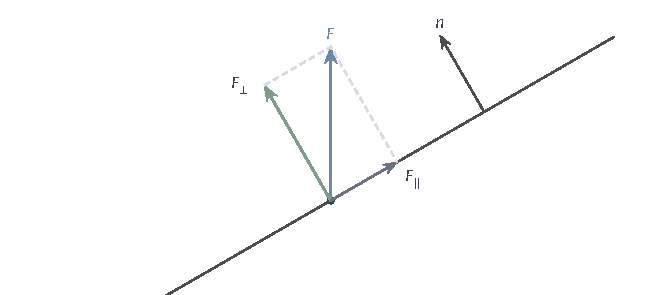
\includegraphics[width=112mm]{figures/00-shared/mathematical-preliminaries-upper/00-shared/tikz/chapter3-concept-processes/normal-projection.pdf}
 \caption{黑斜线表示局部切平面的一个截面，$n$为所选单位法向。向量$F$分为$F_\perp=(F^\top n)n$与切向部分$F_\parallel$；通量使用有符号标量$F^\top n$乘面积，切向部分不贡献。将$n$改为$-n$时标量分量变号，但投影向量$F_\perp$不变，这与直接把场反向不同。}
 \label{fig:analysis-process-normal-projection}
\end{figure}

连续向量场在紧曲面上有界，参数化的有向面积元也连续，因此每片通量都存在。切向分量不贡献通量；反转所选法向则使通量变号。

\subsubsection{积分的性质}

以下运算都在同一曲面、同一法向约定下进行，并假定各法向分量可积。
它们大多可归结为标量函数$\bm F^\top\bm n$的面积积分，直接沿用第一类积分的性质；与方向有关的法向反转和重参数化则需要单独说明。

\paragraph{加法}

向量场相加以后，其法向分量也相加，因此
\[
 \begin{aligned}
 \int_S(\bm F+\bm G)^\top\bm n\,\mathrm dS
 &=\int_S\bm F^\top\bm n\,\mathrm dS\\
 &\quad{}+\int_S\bm G^\top\bm n\,\mathrm dS.
 \end{aligned}
\]
绝对可积性由两项法向分量的绝对值之和控制，积分等式来自标量面积积分的加法性质。
物理上，两股水流叠加后穿过网的水量，等于两股水流分别穿过的水量之和。

\paragraph{减法}

向量场相减以后，其法向分量也相减，因此
\[
 \begin{aligned}
 \int_S(\bm F-\bm G)^\top\bm n\,\mathrm dS
 &=\int_S\bm F^\top\bm n\,\mathrm dS\\
 &\quad{}-\int_S\bm G^\top\bm n\,\mathrm dS.
 \end{aligned}
\]
两项法向分量绝对可积时，它们的差仍绝对可积，积分等式来自标量面积积分的减法性质。

\paragraph{数乘}

对实数$c$，由$(c\bm F)^\top\bm n=c(\bm F^\top\bm n)$，常数可以提出积分号：
\[
 \int_S(c\bm F)^\top\bm n\,\mathrm dS
 =c\int_S\bm F^\top\bm n\,\mathrm dS.
\]
这里缩放的是场，曲面的法向约定保持固定：流速加倍，穿过的水量也加倍。

\paragraph{曲面分割的可加性}

将$S$分为内部不重叠的有限片$S_1,\ldots,S_N$，并在每片采用原定向的限制，则
\[
 \int_S\bm F^\top\bm n\,\mathrm dS
 =\sum_{j=1}^N\int_{S_j}\bm F^\top\bm n\,\mathrm dS.
\]
零面积接缝不贡献积分。
关键在于每片沿用原来的法向：若某片单独反转法向，这一片计入的是反方向的穿越量，加起来就不再是整张曲面的通量。

\paragraph{法向反转}

在场和曲面不变时，把$\bm n$换成$-\bm n$会使通量变号：
\[
 \int_S\bm F^\top(-\bm n)\,\mathrm dS
 =-\int_S\bm F^\top\bm n\,\mathrm dS.
\]
水流本身没有变，变的只是计数方向：例如原法向朝上时，从下往上的穿越原来记为正，现在记为负。
这与第一类积分不同，后者不使用法向，换定向不改变结果。

\paragraph{重参数化}

更换参数时，所选的几何法向保持不变。
由定理~\ref{thm:analysis-surface-reparameterization}，新参数的叉积等于原叉积乘$\det\bm J_T$，
而二维换元公式使用的是$|\det\bm J_T|$。若$\det\bm J_T>0$，两者相同，式~\eqref{eq:analysis-surface-flux}右端不变；
若$\det\bm J_T<0$，例如交换两个参数，新叉积指向相反一侧，按定义中“方向相反时乘$-1$”的约定校正后，结果仍不变。
因此在固定曲面定向并完成这一校正后，通量只依赖曲面、定向和场，与参数选择无关。

\subsubsection{积分的计算}

计算通量分三步：先确定要用哪一侧的法向，再选一个叉积指向该侧的参数化（若指向相反，就在结果前加负号），最后在参数域上累计$\bm F$与有向面积元的内积。

对于图像曲面$z=\psi(x,y)$，第一类积分的计算中已经求出叉积
\[
 \bm r_x\times\bm r_y=(-\psi_x,-\psi_y,1)^\top,
\]
它的第三分量为正，指向上方。
因此取向上法向时，对$\bm F=(P,Q,R)^\top$有
\[
 \int_S\bm F^\top\bm n\,\mathrm dS
 =\iint_D(-P\psi_x-Q\psi_y+R)(x,y,\psi(x,y))\,\mathrm dx\,\mathrm dy.
\]
取向下法向则在右侧加负号。这一式直接使用有向面积元，叉积的长度已经与单位法向的分母抵消，不能再额外乘一次$\sqrt{1+\psi_x^2+\psi_y^2}$。

斜平面片是$\psi(x,y)=x+y$在单位正方形上的图像，可以用它核对通量与投影面积的关系。

\begin{example}[斜平面片上的竖直通量]
\label{ex:analysis-tilted-plane-flux}
取斜平面片$\bm r(u,v)=(u,v,u+v)^\top$、$E=[0,1]^2$和向上单位法向$(-1,-1,1)^\top/\sqrt3$。
对竖直单位场$\bm F=(0,0,1)^\top$，场与参数叉积$(-1,-1,1)^\top$的内积为$1$，故
\[
 \int_S\bm F^\top\bm n\,\mathrm dS
 =\int_0^1\int_0^1 1\,\mathrm du\,\mathrm dv=1.
\]
用面积分开看：这块面的面积为$\sqrt3$（示例~\ref{ex:analysis-tilted-plane-area}），场的法向分量为$\bm F^\top\bm n=1/\sqrt3$，两者相乘为$1$，恰好等于它在$xy$平面上的投影面积。
\end{example}

同样地，平面$z=ax+by+c$在单位圆盘$D$上方的部分对该场的向上通量为$\iint_D1\,\mathrm dx\,\mathrm dy=\pi$，
等于水平投影面积；它的实际面积则为$\pi\sqrt{1+a^2+b^2}$。
这与示例~\ref{ex:analysis-tilted-square-flux}中倾斜屋顶接雨的结果一致：竖直的流只“看见”曲面的水平投影。

对半径为$R$的球面，讨论单位法向量时已算出$(\varphi,\theta)$次序的参数叉积为$R\sin\varphi\,\bm r$，它在参数域内部指向外侧。
下面三个例子都取外法向，依次计算径向场、点源场和恒定场的通量。

\begin{example}[径向场穿过球面]
\label{ex:analysis-radial-field-sphere-flux}
令$\bm F(\bm x)=\bm x/R$。在球面上$\bm F$恰等于外单位法向，$\bm F^\top\bm n=1$，由示例~\ref{ex:analysis-sphere-area}，
\[
 \int_S\bm F^\top\bm n\,\mathrm dS
 =\int_S1\,\mathrm dS=4\pi R^2.
\]
取内法向时通量为$-4\pi R^2$。
\end{example}

这次外向通量与面积相等，是因为法向分量处处为$1$。
一般情形下$|\bm F^\top\bm n|\leq\lVert\bm F\rVert_2$，通量的绝对值不超过场的大小对面积的积分；场的方向偏离法向时，只有法向分量计入通量。

接下来的两个例子形成对比：一个场由原点处的点源发出，另一个场在空间中处处相同。

\begin{example}[点源场的通量与半径无关]
\label{ex:analysis-point-source-sphere-flux}
令$\bm F(\bm x)=\bm x/\lVert\bm x\rVert_2^3$（$\bm x\neq\bm0$），$S$是以原点为中心、半径为$R$的球面，外法向为$\bm n=\bm x/R$。
$\bm F$在不含原点的球面上连续，因而法向分量可积。
在$S$上$\lVert\bm x\rVert_2=R$，故
\[
 \bm F^\top\bm n=\frac{\bm x^\top\bm x}{R^3\cdot R}=\frac1{R^2},
\]
外向通量为$(1/R^2)\cdot4\pi R^2=4\pi$。
\end{example}

球面越大，场越弱，但面积增大的倍数恰好抵消场的减弱，所以通量不随$R$改变：
以点源为中心的球面无论多大，测得的点源单位时间放出的总量都一样。

\begin{example}[恒定场穿过球面的净通量为零]
\label{ex:analysis-constant-field-sphere-flux}
令$\bm F=(0,0,1)^\top$。由$\bm r_\varphi\times\bm r_\theta=R\sin\varphi\,\bm r$，被积函数为
$\bm F^\top(\bm r_\varphi\times\bm r_\theta)=R\sin\varphi\cdot R\cos\varphi=R^2\sin\varphi\cos\varphi$，于是
\[
 \int_S\bm F^\top\bm n\,\mathrm dS
 =\int_0^{2\pi}\int_0^\pi R^2\sin\varphi\cos\varphi\,\mathrm d\varphi\,\mathrm d\theta=0.
\]
分开计算，上半球面$0\leq\varphi\leq\pi/2$的外向通量为
\[
 2\pi R^2\int_0^{\pi/2}\sin\varphi\cos\varphi\,\mathrm d\varphi=\pi R^2,
\]
下半球面$\pi/2\leq\varphi\leq\pi$的外向通量为$-\pi R^2$。
\end{example}

在恒定场中，水从下半球面流入球内，又从上半球面等量流出，球内既不产生也不吸收水，所以闭曲面的净通量为零。
包围点源的球面则有正的净通量。
可见闭曲面的净通量反映它所围区域内部的源与汇；
第~\ref{sec:multivariable-boundary-relations}节将用区域内部的散度累计来计算闭曲面的通量，并核对这里的几个结果。

\FloatBarrier

\section{向量场与微分算子}

定义~\ref{def:multivariable-gradient}把标量函数的各个一阶偏导数排成梯度。现在考虑开集$U$上的向量场$\bm F$，不妨把它想成流体的速度场：$\bm F(\bm x)$是流体在位置$\bm x$处的速度。
对这样的场，有两个自然的局部问题：在一点附近，流体是净流出还是净流入；流体是否绕这一点打转。
两个问题的答案都由$\bm F$各分量的一阶偏导数决定，但用到的偏导数组合不同。
回答前一个问题的是散度，回答后一个问题的是旋度，二者都以向量场为输入；随后的Laplace算子以标量函数为输入，比较函数在一点的值与周围平均值的差别。

\subsection{散度与局部通量}

\paragraph{小立方体的净流出}

设$\bm F=(F_1,F_2,F_3)^\top$是三维流体的速度场。第~\ref{sec:analysis-surface-integration}节定义的通量只取速度的法向分量，原因如下。

在很短的时间$\Delta t$内，穿过面积为$\Delta S$、单位法向为$\bm n$的一小片曲面的流体，占据一个底面积为$\Delta S$、高约为$(\bm F^\top\bm n)\Delta t$的斜柱；所以单位时间穿过这一小片的流体体积约为$(\bm F^\top\bm n)\Delta S$，速度的切向分量只让流体沿曲面滑动，不贡献穿过量。
现在以点$\bm a$为中心取边长为$h$的小立方体，各面与坐标平面平行，估计单位时间从它流出的净体积。

先看与$x$轴垂直的两张面。右面$x=a_1+h/2$的外法向是$\bm e_1$，场在这张面上的法向分量是$F_1$；用面中心的值代表整张面，流出量约为$F_1(\bm a+\tfrac h2\bm e_1)h^2$。
左面$x=a_1-h/2$的外法向是$-\bm e_1$，流出量约为$-F_1(\bm a-\tfrac h2\bm e_1)h^2$；$F_1>0$时这个量为负，表示沿$x$正方向的流动在左面是流入。两面合计为
\[
 \Bigl[F_1\bigl(\bm a+\tfrac h2\bm e_1\bigr)-F_1\bigl(\bm a-\tfrac h2\bm e_1\bigr)\Bigr]h^2
 \approx \partial_1F_1(\bm a)\,h\cdot h^2,
\]
这里用偏导数乘距离$h$近似了$F_1$在两张面中心之间的差。
若$F_1$沿$x$方向增大，从右面的有向流出量与左面的有向流出量之和为正，这对面贡献正的净流出；若$F_1$沿$x$方向不变，流入与流出恰好相等。

另外两对面同样分别给出约$\partial_2F_2(\bm a)h^3$和$\partial_3F_3(\bm a)h^3$。六张面合计后除以体积$h^3$，得到
\[
 \frac{\text{小立方体的净流出}}{\text{小立方体的体积}}
 \approx\partial_1F_1(\bm a)+\partial_2F_2(\bm a)+\partial_3F_3(\bm a).
\]
当$\bm F$连续可微时，可把它在整个小立方体上统一展开为$\bm F(\bm a)+D\bm F(\bm a)(\bm x-\bm a)+o(h)$。每张面的面积为$h^2$，余项对六张面通量的总贡献是$o(h^3)$；常数项在相对两面抵消，线性项给出上面的三个偏导数。除以$h^3$再令$h\to0$，便得到所述极限，无需先使用整个区域上的Gauss公式。右侧的偏导数之和称为散度。
\begin{definition}[散度]
\label{def:multivariable-divergence}
设$U\subseteq\mathbb R^d$为开集，$\bm F=(F_1,\ldots,F_d)^\top:U\to\mathbb R^d$的各分量一阶偏导数存在。
$\bm F$的\term{散度}（divergence）是标量函数
\[
 \operatorname{div}\bm F
 =\nabla\mathbin{\cdot}\bm F
 =\sum_{j=1}^d\partial_jF_j.
\]
\end{definition}
当$\bm F$可微时，这个和也等于Jacobian矩阵$D\bm F$的迹。它只累计对应坐标方向的变化率；非对角偏导数不直接进入净流出率。

\paragraph{源的强度}

按小立方体上的推导，散度是单位体积的净流出率，可以理解为一点处“源”的强度。
$\operatorname{div}\bm F(\bm a)>0$表示$\bm a$附近像有一个源，流体在这里产生并向外流走；$\operatorname{div}\bm F(\bm a)<0$表示这里像一个汇，流入的多于流出的；散度为零表示流入与流出平衡。
若流体不可压缩，内部又没有注入或抽出流体的源和汇，则每个小体积的流入量都等于流出量，速度场的散度处处为零。

下面三个场分别对应均匀膨胀、绕轴转动和整体平移，可以用来检验这一解释。
\begin{example}[径向场、旋转场与常场的散度]
三维径向场$\bm F(x,y,z)=(x,y,z)^\top$满足$\partial_xF_1=\partial_yF_2=\partial_zF_3=1$，所以$\operatorname{div}\bm F=1+1+1=3$：流体从各处均匀地向外膨胀，每单位体积每单位时间多出$3$个单位体积的流体。

旋转场$\bm G(x,y,z)=(-y,x,0)^\top$的第一分量不含$x$，第二分量不含$y$，第三分量为零，所以$\operatorname{div}\bm G=0+0+0=0$：流体绕$z$轴转动，任何小立方体流入多少就流出多少。

常场$\bm H=(1,0,0)^\top$的各分量都是常数，散度同样为$0$：流体整体平移，每个小立方体从左面流入的量都从右面流出。
\end{example}
旋转场和常场都不是零场，散度却都为零。可见散度为零只表示局部净流出率为零，并不表示向量场为零。

二维场$(P,Q)^\top$的散度相应为$P_x+Q_y$，它是小正方形四条边上的净流出除以面积所得的极限；定理~\ref{thm:multivariable-planar-flux}的平面通量公式使用这一标量函数。

\subsection{旋度与局部环流}

\paragraph{小正方形上的环流}

净流出不能描述绕一点旋转的运动。旋转场$\bm G=(-y,x,0)^\top$的散度为零，但在水平平面内沿以$z$轴上一点为圆心的圆周逆时针走一圈，场始终与行进方向相同，环流不为零。
为了度量一点附近的旋转，先在平面上计算小正方形边界的环流。

设平面场为$(P,Q)^\top$，以$\bm a$为中心取边长为$h$的正方形，沿逆时针方向走一圈。

下边从左向右，切向分量是$P$，贡献约$P(\bm a-\tfrac h2\bm e_2)h$；上边从右向左，贡献约$-P(\bm a+\tfrac h2\bm e_2)h$；两者合计约$-\partial_yP(\bm a)h^2$。
右边从下向上，贡献约$Q(\bm a+\tfrac h2\bm e_1)h$；左边从上向下，贡献约$-Q(\bm a-\tfrac h2\bm e_1)h$；两者合计约$\partial_xQ(\bm a)h^2$。四边相加后除以面积$h^2$，得到
\[
 \frac{\text{小正方形边界的逆时针环流}}{\text{小正方形的面积}}
 \approx\partial_xQ(\bm a)-\partial_yP(\bm a).
\]
两项的符号可以这样理解。若$Q$沿$x$方向增大，右边向上的流速比左边大，这一对边推动逆时针转动；若$P$沿$y$方向增大，上边向右的流速比下边大，这一对边推动顺时针转动，所以$\partial_yP$带负号。

在三维空间中，小正方形可以放在分别垂直于三个坐标轴的平面里，行进方向都取从相应坐标轴正方向看的逆时针。
垂直于$z$轴时，平面坐标是$(x,y)$，$(F_1,F_2)$相当于$(P,Q)$，同样的计算给出$\partial_xF_2-\partial_yF_1$；
垂直于$x$轴时，平面坐标的次序是$(y,z)$，$(F_2,F_3)$相当于$(P,Q)$，得到$\partial_yF_3-\partial_zF_2$；
垂直于$y$轴时，平面坐标的次序是$(z,x)$，$(F_3,F_1)$相当于$(P,Q)$，得到$\partial_zF_1-\partial_xF_3$。
这样选取坐标次序，是因为$\bm e_2\times\bm e_3=\bm e_1$、$\bm e_3\times\bm e_1=\bm e_2$：从坐标轴正方向看，第一个平面坐标轴逆时针转过直角得到第二个。
把这三个环流率按$x,y,z$轴的次序排成一个向量，就得到旋度。
\begin{definition}[旋度]
\label{def:multivariable-curl}
设$U\subseteq\mathbb R^3$为开集，$\bm F=(F_1,F_2,F_3)^\top:U\to\mathbb R^3$的各分量一阶偏导数存在。
$\bm F$的\term{旋度}（curl）是向量场
\[
 \operatorname{curl}\bm F=\nabla\times\bm F
 =\begin{pmatrix}
   \partial_yF_3-\partial_zF_2\\
   \partial_zF_1-\partial_xF_3\\
   \partial_xF_2-\partial_yF_1
  \end{pmatrix}.
\]
\end{definition}

\paragraph{旋转的轴与强度}

坐标平面上的三个计算可以推广到任意方向。

设$\bm F$连续可微，$\bm n$是单位向量；在过点$\bm a$且垂直于$\bm n$的平面内，取以$\bm a$为中心的小正方形或小圆周，从$\bm n$的箭头一侧看按逆时针行进。
尺寸趋于零时，环流除以所围面积的极限等于$(\operatorname{curl}\bm F)(\bm a)^\top\bm n$。$\bm n$为坐标轴方向时，这就是上面的计算；一般方向的证明放在Stokes公式之后。

由Cauchy--Schwarz不等式，$(\operatorname{curl}\bm F)^\top\bm n\leq\lVert\operatorname{curl}\bm F\rVert_2$；旋度不为零时，等号当且仅当$\bm n$与旋度同向时成立。
所以旋度的方向是局部旋转最强的转轴，其长度是旋转的强度；转向由右手定则确定：右手大拇指沿旋度方向，其余四指弯曲的方向就是转向。

一个物理图像是放进流水中的小桨轮。让桨轮的转轴沿$\bm n$，水流沿轮缘推动各个叶片；桨轮是否转动、往哪边转，取决于沿轮缘的环流，也就是$(\operatorname{curl}\bm F)^\top\bm n$的符号；转轴与旋度平行时转得最快。
这一图像帮助理解定义，但不代替上面的计算。

先用整体转动和径向膨胀检验这一图像。
\begin{example}[刚体旋转与径向膨胀的旋度]
\label{ex:analysis-rigid-rotation-curl}
整体以角速度$\omega$绕$z$轴旋转的流体，速度场为$\bm F=\omega(-y,x,0)^\top$。代入定义，前两个分量$\partial_yF_3-\partial_zF_2$与$\partial_zF_1-\partial_xF_3$都为零，第三个分量为$\partial_x(\omega x)-\partial_y(-\omega y)=2\omega$，所以$\nabla\times\bm F=(0,0,2\omega)^\top$。
特别地，$\omega=1/2$时$\bm F=(-y/2,x/2,0)^\top$，旋度为$(0,0,1)^\top$。

径向场$(x,y,z)^\top$的第$i$个分量只依赖第$i$个坐标，旋度定义中的每个交叉偏导数都为零，所以旋度为零：流体只向外膨胀而不打转。
\end{example}
刚体旋转的旋度沿转轴，长度是角速度的两倍，与桨轮图像一致。不过，旋度与流线是否弯曲并不是一回事，下面两个场从相反的方向说明这一点。
\begin{example}[剪切流与涡旋场]
剪切流$\bm F=(y,0,0)^\top$的流线都是水平直线。它的偏导数中只有$\partial_yF_1=1$不为零，所以$\nabla\times\bm F=(0,0,-1)^\top$。
物理上，上方的水比下方的水向右流得快，桨轮的上缘被推得更多，从$z$轴正方向看桨轮顺时针转动，与第三分量为负一致。

再看平面上沿同心圆流动的场。

设流体在每个以原点为圆心的圆周上逆时针流动，半径为$r$的圆周上速率为$s(r)>0$，其中$s$可微，即
\[
 \begin{gathered}
(P,Q)^\top=g(r)\,(-y,x)^\top\\
g(r)=\frac{s(r)}r\\
r=\sqrt{x^2+y^2}>0.
 \end{gathered}
\]
由$\partial_xr=x/r$、$\partial_yr=y/r$，有$Q_x=g(r)+g'(r)x^2/r$、$P_y=-g(r)-g'(r)y^2/r$，所以
\[
 Q_x-P_y=2g(r)+rg'(r)=\frac{s(r)}r+s'(r).
\]
第一项$s(r)/r$来自流线的弯曲，第二项$s'(r)$来自不同半径上流速的差别。刚体旋转$s(r)=\omega r$时两项都等于$\omega$，合计$2\omega$，与前例一致。
第~\ref{sec:multivariable-potential-path-independence}节穿孔平面上的涡旋场$(-y,x)^\top/(x^2+y^2)$对应$s(r)=1/r$，两项分别为$1/r^2$与$-1/r^2$，所以在原点以外$Q_x-P_y=0$。
\end{example}
剪切流的流线是直线，旋度却不为零；涡旋场的流线弯曲，在原点以外旋度却为零。后者的原因是：流线弯曲带来的逆时针倾向，恰好被外侧流速较慢带来的顺时针倾向抵消，所以放在原点以外的小桨轮不转。

对二维场$(P,Q)^\top$，平面内需要的是标量$Q_x-P_y$。
把二维场补上为零的第三分量，写成三维场$(P,Q,0)^\top$后，这一标量正是旋度的第三分量，也就是旋度在向上法向$\bm e_3$上的分量。
符号$\nabla\mathbin\cdot$和$\nabla\times$表示这里定义的偏导数组合，不是两个普通数值向量的内积或叉积。


图~\ref{fig:analysis-process-divergence-circulation-fields}在同一个单位圆周上分别观察净流出与切向环流，比较两种微分算子所记录的信息。
\begin{figure*}[!htbp]
 \centering
 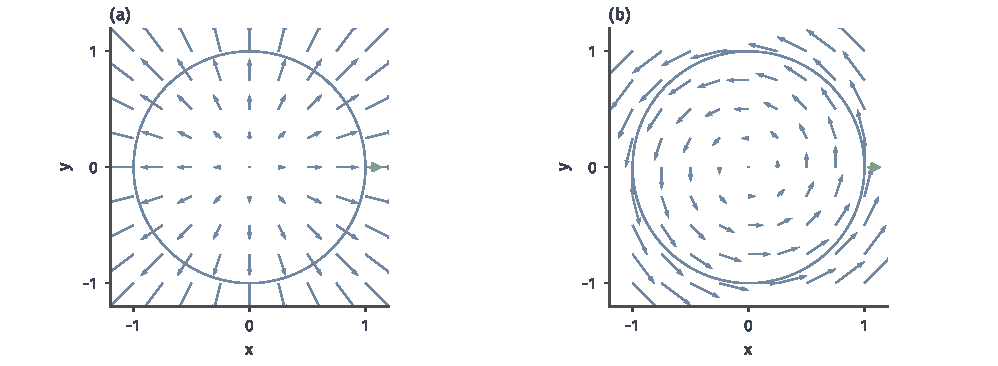
\includegraphics[width=169.0mm]{figures/00-shared/mathematical-preliminaries-upper/00-shared/matplotlib/chapter3-concept-processes/divergence-circulation-fields.pdf}
 \caption{(a) 径向场$(x,y)^\top$的二维散度为$2$、旋转率$Q_x-P_y=0$，圆周外向通量为$2\pi$、环流为零。(b) 旋转场$(-y,x)^\top$的散度为零、旋转率为$2$，通量为零、环流为$2\pi$。绿箭头仅标记外法向；蓝色场箭头按相同常数缩放。零散度不等于零场，也不等于零环流。}
 \label{fig:analysis-process-divergence-circulation-fields}
\end{figure*}

\subsection{Laplace算子与运算关系}

标量函数的梯度是向量场，因此可以对它继续取散度，把各坐标方向的二阶变化相加。
这一复合运算出现在多元分部积分中，也出现在描述热传导和扩散的方程中；它的输入与输出都是标量函数。
\begin{definition}[Laplace算子]
\label{def:multivariable-laplacian}
对开集$U\subseteq\mathbb R^d$上的二阶连续可微标量函数$v$，定义\term{Laplace算子}（Laplacian）为
\[
 \Delta v=\operatorname{div}(\nabla v)
 =\sum_{j=1}^d\partial_j^2v.
\]
\end{definition}
梯度把标量函数变为向量场，散度再把向量场变为标量函数，所以$\Delta v$仍是标量函数；它与输入、输出都是向量场的旋度属于不同类型的运算。

从矩阵表示看，$\Delta v$也是Hessian矩阵的迹。例如$v(\bm x)=\|\bm x\|_2^2$的Hessian为$2\bm I$，所以$\Delta v=2d$。

三个算子还有两条由混合偏导交换直接得到的关系。在三维开集上，若$v\in C^2$，则
\[
 \operatorname{curl}(\nabla v)=\bm0.
\]
例如第三分量是$\partial_x\partial_yv-\partial_y\partial_xv=0$，另两个分量同理。反向由无旋推势函数仍须核对定义域；星形域与有孔域的区别已在路径无关一节说明。

若向量场$\bm F\in C^2$，则
\[
 \operatorname{div}(\operatorname{curl}\bm F)=0.
\]
将旋度的三个分量代入散度，得到六个二阶混合偏导，每一项都与交换求导次序后的另一项异号相消。这里第一个等式的输入是标量函数、输出是零向量，第二个的输入是向量场、输出是零标量，不能混淆对象类型。

\paragraph{与邻域平均值的差}

一元情形中，$v''(a)>0$表示函数在$a$附近向上弯，$v(a)$低于两侧邻点的平均值。多元情形可以做同样的比较。
在$\bm a$的每个坐标方向上各取前后两个邻点$\bm a\pm h\bm e_j$，沿该坐标作二阶Taylor展开：
\[
 v(\bm a+h\bm e_j)+v(\bm a-h\bm e_j)-2v(\bm a)=h^2\partial_j^2v(\bm a)+o(h^2),
\]
一阶项$\pm h\partial_jv(\bm a)$在两点相加时抵消。对$j=1,\ldots,d$求和，再除以邻点个数$2d$，得到
\[
 \frac1{2d}\sum_{j=1}^d\bigl[v(\bm a+h\bm e_j)+v(\bm a-h\bm e_j)\bigr]-v(\bm a)
 =\frac{h^2}{2d}\Delta v(\bm a)+o(h^2).
\]
因此，$h$足够小时，$\Delta v(\bm a)>0$表示$v(\bm a)$低于周围邻点的平均值，$\Delta v(\bm a)<0$表示高于平均值；$\Delta v(\bm a)=0$表示二者之差是$o(h^2)$，在这一精度下相等。

下面用两个二次函数直接比较邻点平均值与中心值。
\begin{example}[二次函数的邻点平均]
取$v(x,y,z)=x^2+y^2+z^2$，则$\Delta v=2+2+2=6$。在原点，$v(\bm0)=0$；六个邻点$\pm h\bm e_j$上的值都是$h^2$，所以邻点平均值比中心值高$h^2$，恰等于$\frac{h^2}{2d}\Delta v=\frac{h^2}6\cdot6$。二次函数的Taylor展开没有余项，等式精确成立。

再取$v(x,y)=x^2-y^2$，则$\Delta v=2-2=0$。原点的四个邻点$(\pm h,0)$与$(0,\pm h)$上的取值为$h^2,h^2,-h^2,-h^2$，平均值恰为$0=v(\bm0)$。
\end{example}
第二个函数在$x$方向向上弯、在$y$方向向下弯，两种弯曲正好抵消。Laplace算子记录的是各坐标方向弯曲的总和，不能据此判断每个方向各自的弯曲。

\paragraph{热传导中的含义}

设$u(t,\bm x)$是时刻$t$物体内位置$\bm x$处的温度，它对$\bm x$二阶连续可微。热量从高温处流向低温处，Fourier热传导定律把单位时间穿过单位面积的热流写成$\bm q=-k\nabla u$，其中常数$k>0$为导热系数，$\nabla$只作用于空间变量$\bm x$\scite{math-openstax-calculus3}。
由散度的含义，单位体积的热量净流出率为$\operatorname{div}\bm q=-k\Delta u$。没有热源时，单位体积内热量的增加率等于净流入率$-\operatorname{div}\bm q=k\Delta u$；再除以单位体积的热容$c>0$，得到温度的变化率
\[
 \partial_tu=\frac kc\,\Delta u,
\]
这就是热传导方程。

这个方程说明温度怎样随时间变化。比周围平均更冷的点满足$\Delta u>0$，会从周围吸收热量而升温；比周围平均更热的点满足$\Delta u<0$，会降温；温度分布因而逐渐被抹平。
温度不再随时间变化时，处处有$\Delta u=0$；按邻域平均值的公式，每点的温度在上述精度下等于周围的平均。这里的Fourier定律是物理模型，本节只用它说明$\Delta$的含义。

\section{区域与边界的积分关系}
\label{sec:multivariable-boundary-relations}

一元微积分基本定理说，若$f$在$[a,b]$上连续可微，则导数$f'$在区间上的积分等于$f(b)-f(a)$：区间内部各点的变化率累计起来，只剩下两个端点上的函数值。
区间的边界就是这两个端点，所以$f(b)-f(a)$也可以读成带符号的边界求和：右端点记正号，左端点记负号。
路径积分基本定理（式~\eqref{eq:analysis-line-integral-gradient}）把同样的关系搬到路径上：梯度场沿路径的积分，等于势函数在终点与起点的值之差。

本节把这种“内部导数的累计等于边界上的累计”的关系推广到平面区域、空间区域和曲面。
三种推广共用一个思路。先把对象切成许多小块；在每个小块上，某个导数乘小块的大小，近似等于向量场沿小块边界的累计。
相邻两块的公共边界被两块各算一次，两次的方向相反，相加后抵消，最后只剩下整个对象的外边界。
按边界的类型，本节回答三个问题：平面区域上的积分何时等于边界路径积分，这是Green公式；空间区域上的积分何时等于边界曲面积分，这是Gauss公式；曲面上的积分何时等于曲面边界的路径积分，这是Stokes公式。

这些公式中的被积对象不能互换。沿边界的环流累计向量场的切向分量，对应的内部量是旋度，它衡量场绕一点旋转的强度；
穿过边界的通量累计向量场的法向分量，对应的内部量是散度，它衡量场从一点向外发散的强度。

前一节已从局部变化定义散度、旋度与Laplace算子。下面先规定边界的方向，再给出内部与边界之间的积分关系。
所有参数积分沿用本章的Riemann积分。经典公式的组织参考向量微积分教材\scite{math-openstax-calculus3}。

\paragraph{边界的定向}

将一个区域分成相邻小块时，公共边或公共面不属于原区域的外边界。
要使这些内部贡献相消，各小块必须采用相容的方向；同时，每个小块的方向还要与小块上局部计算所用的方向一致：环流按逆时针计算，通量按外法向计算。
下面依次规定平面区域边界的行进方向、区域边界的外法向，以及定向曲面边界的行进方向。

\paragraph{平面区域的正向边界}

平面区域的边界是路径，所以先规定沿边界行进的方向。本节考虑的平面区域，边界由若干条简单闭曲线组成；简单闭曲线指除首尾相合外不自交的闭曲线。
对有界平面区域，取边界方向使沿曲线前进时区域总在左侧，称为正向边界。
沿单位圆逆时针行走，单位圆盘始终在左手边，所以圆盘的正向边界是逆时针方向。

有孔洞时，外边界仍是逆时针；围绕孔洞的内边界要使区域而非孔洞留在左侧，因而是顺时针。
例如圆环$1<x^2+y^2<4$的外圈$r=2$逆时针、内圈$r=1$顺时针，两圈边界方向相反。
这个约定与小块相消的要求一致：把圆环切成许多小块，每块都按逆时针走边界，内部公共边相互抵消后，剩在孔洞边上的那些边恰好被顺时针走过。

边界由多段光滑弧组成时，按这一方向逐段相接，转角处不另加积分项。
一般地，相邻平面小块各自采用正向边界时，共同边被沿相反方向走过，两个有向路径积分恰好抵消。

\paragraph{区域边界的外法向}

通量需要的是法向，而不是边界的行进方向。空间区域的外单位法向从内部指向外部；有孔洞时，孔洞边界的外法向指向孔洞。
例如球壳$1<\lVert\bm x\rVert_2<2$在外球面上的外法向背离原点，在内球面上的外法向指向原点。
相邻子区域的公共面上，两侧子区域的外法向相反，所以内部通量相消。

平面区域边界上的外单位法向按同样方式规定，只是通量沿边界按弧长累计。
外法向与正向边界的单位切向量$\bm\tau=(\tau_1,\tau_2)^\top$有固定关系：区域在行进方向的左侧，外侧就在右侧，所以把$\bm\tau$顺时针转过直角就得到外法向$\bm n=(\tau_2,-\tau_1)^\top$。
例如在单位圆的点$(1,0)$处，逆时针的切向量是$(0,1)^\top$，按此公式得到$(1,0)^\top$，确实指向圆外。

\paragraph{定向曲面边界的诱导方向}

曲面取定单位法向$\bm n$后，其边界路径的方向不能再任意选择。
边界的正向按右手约定确定：右手大拇指朝法向，其余手指弯曲的方向为正向，称为由法向诱导的方向，简称诱导方向。
等价地，沿边界前进并把头朝向法向时，曲面留在左侧。面朝前进方向$\bm f$、头顶朝$\bm u$站立时，左手方向是$\bm u\times\bm f$；用这个叉积可以核对具体例子。

下面用这个叉积核对两张以单位圆为边界的曲面，后面检验Stokes公式时会用到它们。
\begin{example}[向上圆盘与外向上半球面的诱导方向]
\label{ex:analysis-hemisphere-induced-orientation}
对取向上法向$\bm e_3$的单位圆盘，在边界点$(1,0,0)$处取前进方向$\bm f=\bm e_2$，左手方向为$\bm e_3\times\bm e_2=-\bm e_1$，指向圆盘内部。所以诱导方向是从上方看逆时针。

对取外法向的上半单位球面，赤道上的点$(1,0,0)$处外法向是$\bm e_1$。同样取前进方向$\bm f=\bm e_2$，左手方向为$\bm e_1\times\bm e_2=\bm e_3$，正指向半球面所在的上方。所以它的诱导方向也是从上方看逆时针，与向上圆盘的边界方向相同。
\end{example}
两张曲面在边界点处的法向不同，曲面伸出的方向也不同；但二者都满足“头朝法向时曲面在左侧”，所以诱导出同一个边界方向。

若翻转曲面法向，边界的诱导方向也随之翻转。分片曲面的定向相容，指相邻曲面片在公共边上诱导出相反的行进方向。
这时公共边上的路径积分相消，只留下整张曲面的真正边界。


图~\ref{fig:analysis-process-boundary-orientation-cancellation}把相容方向的作用画出来：只有内部公共边相消，才会只剩下整个对象的外边界。
\begin{figure}[!htbp]
 \centering
 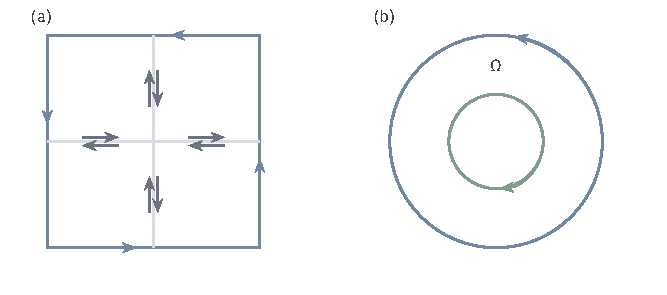
\includegraphics[width=112mm]{figures/00-shared/mathematical-preliminaries-upper/00-shared/tikz/chapter3-concept-processes/boundary-orientation-cancellation.pdf}
 \caption{(a) 四个小正方形各取逆时针正向，共同边被沿相反方向走过；灰箭头略错开以便辨认，实际是同一条边。相加后只留下蓝色外边界。(b) 圆环的外边界逆时针、孔洞边界顺时针，沿任一边界前进时区域均在左侧。曲面拼片时也按公共边相反方向保证Stokes边界项相消。}
 \label{fig:analysis-process-boundary-orientation-cancellation}
\end{figure}

\subsection{Green公式与平面边界}

在平面上，区域的边界是一维路径。对同一个二维向量场，可以沿边界累计切向分量，得到环流；也可以累计外法向分量，得到通量。
两种边界积分分别对应区域内部的$Q_x-P_y$和散度$P_x+Q_y$。

\subsubsection{Green公式的环流形式}

旋度一节在小正方形上算出：逆时针环流约等于$Q_x-P_y$乘正方形面积。
把区域$\Omega$划分成许多小正方形（靠近弯曲边界处是不规则的小块），对每块写出这一近似再相加。
相邻两块的公共边在两块中方向相反，贡献抵消，剩下的只有沿$\Omega$正向边界的环流；另一侧各块“$Q_x-P_y$乘面积”之和，则是区域积分的近似和。
Green公式说明，在适当条件下这一近似在加细后成为精确等式：区域内各处微小旋转的累计，等于沿边界走一圈的总环流。
\begin{theorem}[Green公式]
\label{thm:multivariable-green}
设$\Omega\subseteq\mathbb R^2$为有界开区域，边界由有限条分段$C^1$简单闭曲线组成，
且区域在每段光滑边界附近位于边界的一侧。边界取正向，即外边界逆时针、孔洞边界顺时针。
若二维向量场$\bm F=(P,Q)^\top$在$\overline\Omega$的开邻域内连续可微，则\term{Green公式}（Green's theorem）给出
\begin{equation}
 \oint_{\partial\Omega}P\,\mathrm dx+Q\,\mathrm dy
 =\iint_\Omega\left(\frac{\partial Q}{\partial x}-\frac{\partial P}{\partial y}\right)\,\mathrm dx\,\mathrm dy.
 \label{eq:multivariable-green}
\end{equation}
\end{theorem}
左侧是向量场的切向路径积分；右侧是标量函数$Q_x-P_y$的区域积分。
在矩形上，二者的等式可以直接由一元基本定理和连续函数的累次积分公式推出。
\begin{proof}[矩形情形的证明]
取$\Omega=(a,b)\times(c,d)$，先写出左侧沿四条边的贡献。下边$(t,c)$、$a\leq t\leq b$从左向右，$\mathrm dy=0$，贡献$\int_a^bP(x,c)\,\mathrm dx$；
上边从$(b,d)$走到$(a,d)$，贡献$-\int_a^bP(x,d)\,\mathrm dx$；右边从下向上，贡献$\int_c^dQ(b,y)\,\mathrm dy$；左边从上向下，贡献$-\int_c^dQ(a,y)\,\mathrm dy$。
水平边上$\mathrm dy=0$，竖直边上$\mathrm dx=0$，所以$Q$只在竖直边出现，$P$只在水平边出现。

再看右侧。场在闭矩形附近连续可微，以下被积函数均可积。固定$x$，对$y$用一元基本定理得$\int_c^d\partial_yP(x,y)\,\mathrm dy=P(x,d)-P(x,c)$；再对$x$积分，并由连续函数的累次积分公式换成区域积分。对$Q$则先固定$y$、对$x$积分。于是
\[
 \begin{aligned}
 -\iint_\Omega\partial_yP\,\mathrm dx\,\mathrm dy
 &=\int_a^b[P(x,c)-P(x,d)]\,\mathrm dx,\\
 \iint_\Omega\partial_xQ\,\mathrm dx\,\mathrm dy
 &=\int_c^d[Q(b,y)-Q(a,y)]\,\mathrm dy.
 \end{aligned}
\]
第一行恰是下边与上边的两项，第二行恰是右边与左边的两项。
四项合起来，正是沿下、右、上、左四条边逆时针行进得到的路径积分。
\end{proof}
有限个矩形拼接时，公共边上的积分因方向相反而抵消。
一般规则区域的证明还需处理区域分片及边界逼近误差，不能仅凭小矩形上的等式完成；这里引用一般形式，完整论证可参考向量微积分教材\scite{math-strang1991calculus}。

先用旋转场在单位圆盘上核对公式两侧，并观察边界方向的作用。
\begin{example}[旋转场在单位圆盘上的Green公式]
\label{ex:analysis-rotation-field-green-disk}
取$\bm F=(P,Q)^\top=(-y,x)^\top$，$\Omega$为单位圆盘。$\bm F$在整个平面上连续可微，定理条件满足。
右侧被积函数为$Q_x-P_y=1-(-1)=2$，区域积分为$2\cdot\pi=2\pi$。
左侧取逆时针边界$\gamma(t)=(\cos t,\sin t)^\top$，$0\leq t\leq2\pi$，则$\bm F(\gamma(t))^\top\gamma'(t)=\sin^2t+\cos^2t=1$，积分同样为$2\pi$。
若把圆周改为顺时针，左侧变为$-2\pi$，右侧仍为$2\pi$，等式不再成立。
\end{example}
区域积分不含方向信息，边界积分却随方向反转而变号；Green公式的符号由正向边界的约定决定。

Green公式也可以反过来使用：选一个满足$Q_x-P_y\equiv1$的场，右侧就是区域的面积，于是面积可以由边界环流算出。
\begin{example}[用边界计算面积]
\label{ex:analysis-green-area-formula}
设$\Omega$满足定理~\ref{thm:multivariable-green}的条件。取$P=-y/2$、$Q=x/2$，则$Q_x-P_y=1$，Green公式给出
\[
 \operatorname{area}(\Omega)=\frac12\oint_{\partial\Omega}x\,\mathrm dy-y\,\mathrm dx.
\]
对半轴为$\alpha,\beta>0$的椭圆区域，正向边界取$\gamma(t)=(\alpha\cos t,\beta\sin t)^\top$、$0\leq t\leq2\pi$。这时$\mathrm dx=-\alpha\sin t\,\mathrm dt$、$\mathrm dy=\beta\cos t\,\mathrm dt$，
\[
 x\,\mathrm dy-y\,\mathrm dx=(\alpha\beta\cos^2t+\alpha\beta\sin^2t)\,\mathrm dt=\alpha\beta\,\mathrm dt,
\]
所以面积为$\frac12\cdot2\pi\alpha\beta=\pi\alpha\beta$。
\end{example}
这个公式只需要沿边界走一圈、记录坐标与位移，就能得到所围面积；机械求积仪正是按这一原理工作的。

定理要求场在$\overline\Omega$的开邻域内连续可微。区域包含场的奇点时，这一条件不再满足，下面的例子说明它不能省略。
\begin{example}[有孔区域上的涡旋场]
\label{ex:analysis-annulus-vortex-green}
第~\ref{sec:multivariable-potential-path-independence}节的穿孔平面反例中，$\bm F=(-y,x)^\top/(x^2+y^2)$在原点以外满足$Q_x-P_y=0$，但沿单位圆逆时针一周的环流为$2\pi$。

取圆环$\Omega=\{1<x^2+y^2<4\}$。它的闭包不含原点，$\bm F$在$\overline\Omega$的一个开邻域内连续可微，Green公式适用，右侧为$0$。
左侧由两圈组成。外圈$r=2$逆时针，参数化为$(2\cos t,2\sin t)^\top$，此时$\bm F=(-\sin t,\cos t)^\top/2$，与速度$(-2\sin t,2\cos t)^\top$的内积为$1$，环流为$2\pi$；内圈$r=1$按正向取顺时针，环流为$-2\pi$。两者相加为零，与右侧一致。
\end{example}
外圈逆时针为$2\pi$、内圈顺时针为$-2\pi$，也就是说，两条圆周按同一逆时针方向走时环流都是$2\pi$。环流来自场在原点处的奇异，而不是来自圆环内部。
单位圆盘含有原点，$\bm F$在那里无定义，不满足Green公式的条件，所以不能由$Q_x-P_y=0$推出单位圆上的环流为零。

\subsubsection{Green公式的通量形式}

现在把平面向量场想成薄层流体的速度场，问单位时间有多少流体穿过区域边界流出。
每个小正方形的净流出约等于散度乘面积；相邻两块的公共边上外法向相反，一块的流出就是另一块的流入，相加后抵消。
因此可以预期：区域内部源强度的总和，等于穿过边界的净流出。

计算通量需要把场投影到外法向上。正向边界的有向位移是$\bm\tau\,\mathrm ds=(\mathrm dx,\mathrm dy)^\top$，而外法向由$\bm\tau$顺时针转过直角得到，因此
\[
 \bm n\,\mathrm ds=(\mathrm dy,-\mathrm dx)^\top.
\]
这一关系把法向通量写成切向路径积分，从而可以使用Green公式。
\begin{theorem}[平面区域的通量公式]
\label{thm:multivariable-planar-flux}
在与Green公式相同的区域条件下，若$\bm F=(F_1,F_2)^\top$在$\overline\Omega$的开邻域内连续可微，
$\bm n$是边界的外单位法向，则
\[
 \int_{\partial\Omega}\bm F^\top\bm n\,\mathrm ds
 =\iint_\Omega\operatorname{div}\bm F\,\mathrm dx\,\mathrm dy.
\]
\end{theorem}
\begin{proof}
利用外法向与正向边界的关系，$\bm F^\top\bm n\,\mathrm ds=F_1\,\mathrm dy-F_2\,\mathrm dx$，所以左侧等于
$\oint_{\partial\Omega}(-F_2)\,\mathrm dx+F_1\,\mathrm dy$。
在Green公式中取$(P,Q)=(-F_2,F_1)$，右侧被积函数为$Q_x-P_y=\partial_xF_1+\partial_yF_2=\operatorname{div}\bm F$。
\end{proof}
这也是二维的散度公式。它与环流形式使用相同的区域条件，但累计的边界分量和内部导数不同。

下面在单位圆盘上比较两个场的通量：一个从各处均匀发散，一个只绕原点打转。
\begin{example}[单位圆盘上径向场与旋转场的通量]
取$\bm F(x,y)=(x,y)^\top$，$\Omega$为单位圆盘。散度为$1+1=2$，区域积分为$2\pi$。
边界参数化为$\gamma(t)=(\cos t,\sin t)^\top$，$0\leq t\leq2\pi$，外法向$\bm n=\gamma(t)$，$\mathrm ds=\mathrm dt$，且$\bm F^\top\bm n=\cos^2t+\sin^2t=1$，所以边界通量也为$2\pi$。若改取内法向，通量变为$-2\pi$。

再取旋转场$\bm G=(-y,x)^\top$。它的散度为$0+0=0$；在单位圆上$\bm G^\top\bm n=-y\cdot x+x\cdot y=0$，通量为零，两侧一致。它的环流却是示例~\ref{ex:analysis-rotation-field-green-disk}算出的$2\pi$。
\end{example}
径向场好比流体在圆盘内各处均匀产生，产生的总量全部从圆周流出。旋转场则像杯中被搅动的水：水在杯中打转，却没有流出杯壁。通量与环流记录的是边界上两个不同的分量。

\subsection{Gauss公式与封闭曲面}

将平面区域换成三维空间区域后，边界从曲线变成闭曲面。
对应关系仍然是内部散度的积分等于边界净通量；由这一关系还可以推出多元函数的分部积分公式。

\subsubsection{Gauss公式}

仍把$\bm F$看作流体的速度场。区域$\Omega$内各处的散度给出单位体积的产生率，其体积积分是单位时间在$\Omega$内产生的流体总量。
流体总量守恒时，新产生的流体只能穿过边界离开，所以这个总量应等于穿过$\partial\Omega$的外向净通量。
从计算上看，把$\Omega$切成小立方体，每块的净流出约等于散度乘体积；相邻两块的公共面上外法向相反，流出与流入相消，只留下外边界上的通量。
静电学中有同样的关系：电场穿过闭曲面的通量，由闭曲面内的总电荷决定\scite{math-openstax-calculus3}。
Gauss散度定理给出这一平衡精确成立的条件。
\begin{theorem}[Gauss散度定理]
\label{thm:analysis-divergence-theorem}
设$\Omega\subseteq\mathbb R^3$为有界开区域，其边界是由有限个正则$C^1$曲面片组成的闭曲面。
各片内部互不相交，接缝为有限条分段$C^1$曲线及有限个点；在每个光滑边界点附近，区域位于边界的一侧。
若向量场$\bm F$在$\overline\Omega$的一个开邻域内连续可微，则\term{散度定理}（divergence theorem）给出
\begin{equation}
  \int_{\Omega}\nabla\mathbin{\cdot}\bm F\,\mathrm d\bm x
  =\int_{\partial\Omega}\bm F^\top\bm n\,\mathrm dS,
 \label{eq:analysis-divergence-theorem}
\end{equation}
其中$\bm n$是光滑边界片上的外单位法向，$\mathrm dS$为面积元素。
\end{theorem}
光滑有界区域和通常的多面体满足这些条件。接缝的曲面面积为零，不影响通量积分；$\bm F$及其偏导数在紧集$\overline\Omega$上连续因而有界，所以两侧积分都有限。
左侧累计向量场的局部净流出率，右侧累计穿过整个外边界的净通量。

对长方体，这一等式不需要借助一般曲面逼近，可以逐坐标证明；证明正是把散度一节中小立方体上的近似计算改写成精确等式。
\begin{proof}[长方体情形的证明]
取$\Omega=(a,b)\times(c,d)\times(e,f)$。
固定$(y,z)$，对$x$用一元基本定理，再由连续函数的累次积分公式对$(y,z)$积分，得到
\[
 \int_\Omega\partial_xF_1\,\mathrm d\bm x
 =\int_c^d\int_e^f
   [F_1(b,y,z)-F_1(a,y,z)]\,\mathrm dz\,\mathrm dy.
\]
在$x=b$面上外法向为$(1,0,0)^\top$，$\bm F^\top\bm n=F_1$；在$x=a$面上外法向为$(-1,0,0)^\top$，$\bm F^\top\bm n=-F_1$。所以右侧正是这两张面的外向通量之和。
同样，$\partial_yF_2$的体积积分等于$y=d$与$y=c$两面的通量之和，
$\partial_zF_3$的体积积分等于$z=f$与$z=e$两面的通量之和。在其余各面上，相应分量与法向垂直，不贡献这一项。
三式相加，左侧为散度的体积积分，右侧为六张面的全部外向通量。
\end{proof}
拼接长方体时，公共面上的外法向相反，内部通量恰好抵消。
从长方体推广到定理中的一般规则区域，还需对边界分片和逼近作严格处理；一般形式在这里引用，证明可参考向量微积分教材\scite{math-strang1991calculus}。
无界区域、弱导数或更不规则的边界，需要另用相应版本，不能由长方体情形直接推出。


图~\ref{fig:analysis-process-gauss-shared-face}显示体积小块相加时，共同面上的两份通量为什么消失。
\begin{figure}[!htbp]
 \centering
 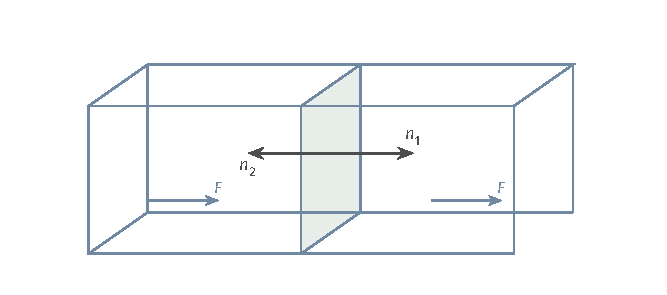
\includegraphics[width=112mm]{figures/00-shared/mathematical-preliminaries-upper/00-shared/tikz/chapter3-concept-processes/gauss-shared-face.pdf}
 \caption{两个相邻单位立方体共用绿色面，图用斜投影表示三维几何。取常场$F=(1,0,0)^\top$，共同面上两侧外法向为$n_1=(1,0,0)^\top$与$n_2=-n_1$，对应通量为$1,-1$，相加抵消。整体外向净通量也为零，与散度为零一致；一般区域的散度定理仍需要前述条件与证明。}
 \label{fig:analysis-process-gauss-shared-face}
\end{figure}

先用一个答案已知的计算核对散度定理。
\begin{example}[用散度定理核对球面面积]
设$B_R$是以原点为中心、半径$R>0$的球，边界球面取外法向。令$\bm F(\bm x)=\bm x/R$，它在整个$\mathbb R^3$上连续可微。
球面上$\bm n=\bm x/R=\bm F$，所以$\bm F^\top\bm n=1$，外向通量等于球面面积。
另一方面，$\operatorname{div}\bm F=3/R$，散度定理给出
\[
 \int_{\partial B_R}\bm F^\top\bm n\,\mathrm dS
 =\frac3R\operatorname{vol}(B_R)
 =\frac3R\cdot\frac{4\pi R^3}3=4\pi R^2.
\]
\end{example}
这里的球体积已在第~\ref{sec:classical-change-variables}节用球坐标算出；所得结果与第~\ref{sec:analysis-surface-integration}节直接参数化球面求得的面积一致。

定理要求$\bm F$在$\overline\Omega$的一个开邻域内连续可微。点源场在原点无定义，下面用它检查这一条件的作用。
\begin{example}[点源的通量]
\label{ex:analysis-point-source-flux}
在$\mathbb R^3\setminus\{\bm0\}$上取$\bm F(\bm x)=\bm x/\lVert\bm x\rVert_2^3$，记$r=\lVert\bm x\rVert_2$。由$\partial_jr=x_j/r$，
\[
 \begin{gathered}
\partial_j\Bigl(\frac{x_j}{r^3}\Bigr)=\frac1{r^3}-\frac{3x_j^2}{r^5}\\
\operatorname{div}\bm F=\frac3{r^3}-\frac{3r^2}{r^5}=0.
 \end{gathered}
\]
但在半径为$R$的球面上，外法向为$\bm x/R$，$\bm F^\top\bm n=1/R^2$，外向通量为$4\pi R^2/R^2=4\pi$。
这并不与散度定理矛盾：球体含有原点，而$\bm F$在原点无定义，定理的条件不满足。

对不含原点的球壳$R_1<r<R_2$，定理适用，左侧为零。外球面的外向通量为$4\pi$；内球面的外法向指向原点，通量为$-4\pi$；两者相加确为零。
\end{example}
所以以原点为中心的球面上的通量都是$4\pi$，与半径无关：场在原点以外处处无源，全部通量都来自原点处的点源。
静电学中，位于原点的点电荷$q$产生的电场是$\frac{q}{4\pi\varepsilon_0}\bm F$，其中$\varepsilon_0$为真空介电常数；它穿过以原点为中心的球面的通量为$q/\varepsilon_0$，这就是Gauss定律在点电荷上的形式。

\paragraph{散度是通量密度}

已证明的长方体情形，足以把散度一节的近似推导变成精确结论。
设$\bm F$在开集$U$上连续可微，$\bm a\in U$，$Q_h$是以$\bm a$为中心、边长为$h$的立方体；$h$足够小时$\overline{Q_h}\subseteq U$。由长方体上的Gauss公式，
\[
 \frac1{h^3}\int_{\partial Q_h}\bm F^\top\bm n\,\mathrm dS
 =\frac1{h^3}\int_{Q_h}\operatorname{div}\bm F\,\mathrm d\bm x.
\]
右侧是散度在$Q_h$上的平均值，它与$\operatorname{div}\bm F(\bm a)$的差不超过$\sup_{Q_h}|\operatorname{div}\bm F-\operatorname{div}\bm F(\bm a)|$。散度连续，所以$h\to0$时这个上界趋于零，平均值趋于$\operatorname{div}\bm F(\bm a)$。

这说明散度确实是“单位体积的净流出”的极限。把立方体换成以$\bm a$为中心的小球，用一般的Gauss公式可以得到同样的极限。小球的取法不依赖坐标轴，所以散度描述的是场本身的性质，不依赖坐标系的方向。

\subsection{Stokes公式与曲面的边界}

Gauss公式要求闭曲面围成空间区域。另一类问题只给一张有边界的定向曲面，要求比较曲面上的旋转累计与边界环流。
这时使用旋度在曲面法向上的分量，不需要先把曲面补成闭曲面。

\subsubsection{Stokes公式}

在$z=0$平面上取向上法向时，旋度的法向分量$(\nabla\times\bm F)^\top\bm e_3$就是Green公式中的$Q_x-P_y$。
对空间中的弯曲曲面，可以把它切成许多很小的曲面片，每片近似是一小块平面。在法向为$\bm n$的小平面片上，边界环流约等于$(\nabla\times\bm F)^\top\bm n$乘面积。
各片采用相容定向时，相邻两片的公共边被沿相反方向走过，环流相消，只剩整张曲面的边界。
用桨轮的图像说：在曲面上各处放置转轴沿法向的小桨轮，它们感受到的旋转强度按面积累加，总和等于沿曲面边缘走一圈的环流。
Stokes公式把这一关系写成精确等式，同时要求法向与边界方向相容。
\begin{theorem}[Stokes定理]
\label{thm:multivariable-stokes}
设$S\subseteq\mathbb R^3$为紧致、可定向的分片$C^2$曲面，边界由有限条分段$C^1$简单闭曲线组成。
各光滑曲面片选取连续且片间定向相容的单位法向$\bm n$，边界采用其诱导方向。
若向量场$\bm F$在$S$的开邻域内连续可微，则\term{Stokes公式}（Stokes' theorem）给出
\begin{equation}
 \oint_{\partial S}\bm F^\top\,\mathrm d\bm r
 =\int_S(\nabla\times\bm F)^\top\bm n\,\mathrm dS.
 \label{eq:multivariable-stokes}
\end{equation}
\end{theorem}
这里的“可定向”要求各曲面片能相容地选择法向，使公共边上的诱导方向相反；有折角的接缝处不要求存在唯一法向。
两侧都为标量：左侧是原向量场的边界环流，右侧是其旋度穿过曲面的通量。

在一张参数曲面片上，可以把公式归结为参数平面上的Green公式。
设参数域$D$满足Green公式的区域条件，$\bm r(u,v)$在$D$的邻域内二阶连续可微、在内部正则且一一对应，并采用$\bm r_u\times\bm r_v$确定的定向。
还要求$\partial D$的正向经$\bm r$对应曲面片边界的诱导方向，从而可以把边界路径积分放到$\partial D$上计算。
这里的$u,v$是曲面的局部参数。记
\[
 \begin{aligned}
 A(u,v)&=\bm F(\bm r(u,v))^\top\bm r_u(u,v),\\
 B(u,v)&=\bm F(\bm r(u,v))^\top\bm r_v(u,v).
 \end{aligned}
\]

先处理左侧。若$(u(t),v(t))$沿$\partial D$行进，曲面边界上对应的点是$\bm r(u(t),v(t))$，由链式法则，其速度为$\bm r_uu'(t)+\bm r_vv'(t)$。
与$\bm F$取内积，得$\bm F^\top\mathrm d\bm r=A\,\mathrm du+B\,\mathrm dv$，所以左侧等于参数平面上的路径积分$\oint_{\partial D}A\,\mathrm du+B\,\mathrm dv$。

再计算参数平面上Green公式右侧的被积函数$\partial_uB-\partial_vA$。记$\bm J_{\bm F}$为$\bm F$的Jacobian矩阵，其元素为$(\bm J_{\bm F})_{i,j}=\partial_jF_i$。由链式法则和乘积法则，
\[
 \begin{aligned}
 \partial_uB&=(\bm J_{\bm F}\bm r_u)^\top\bm r_v+\bm F^\top\bm r_{vu},\\
 \partial_vA&=(\bm J_{\bm F}\bm r_v)^\top\bm r_u+\bm F^\top\bm r_{uv},
 \end{aligned}
\]
其中$\bm J_{\bm F}$与$\bm F$在$\bm r(u,v)$处取值。$\bm r$二阶连续可微，混合偏导相等，$\bm r_{uv}=\bm r_{vu}$，所以两式相减时含二阶导数的项抵消。
又$(\bm J_{\bm F}\bm r_u)^\top\bm r_v=\bm r_v^\top\bm J_{\bm F}\bm r_u$、$(\bm J_{\bm F}\bm r_v)^\top\bm r_u=\bm r_v^\top\bm J_{\bm F}^\top\bm r_u$，于是
\[
 \partial_uB-\partial_vA=\bm r_v^\top(\bm J_{\bm F}-\bm J_{\bm F}^\top)\bm r_u.
\]

接下来把右端写成旋度。反对称矩阵$\bm W=\bm J_{\bm F}-\bm J_{\bm F}^\top$的元素为$\bm W_{i,j}=\partial_jF_i-\partial_iF_j$；逐个分量对照旋度的定义可以验证，对任意$\bm a\in\mathbb R^3$都有$\bm W\bm a=(\nabla\times\bm F)\times\bm a$。
再用混合积的轮换关系$\bm b^\top(\bm c\times\bm a)=\bm c^\top(\bm a\times\bm b)$（两边都等于以$\bm a,\bm b,\bm c$为列的行列式），取$\bm a=\bm r_u$、$\bm b=\bm r_v$、$\bm c=\nabla\times\bm F$，得到
\[
 \partial_uB-\partial_vA
 =\bigl(\operatorname{curl}\bm F\bigr)(\bm r(u,v))^\top
   (\bm r_u\times\bm r_v).
\]
右端乘$\mathrm du\,\mathrm dv$，正是曲面通量积分（式~\eqref{eq:analysis-surface-flux}）中的被积项。

$A,B$由连续可微的$\bm F$与二阶连续可微的$\bm r$及其一阶导数复合、相乘而成，在$D$的邻域内连续可微，所以参数平面上的Green公式适用；它给出该曲面片上的Stokes公式。
对有限张相容定向的曲面片，公共边的路径积分相消，只剩整张曲面的边界。
一般分片曲面的完整论证还需核对曲面覆盖及接缝条件；以上推导只说明参数片上的机制，一般定理可参考向量微积分教材\scite{math-strang1991calculus}。

\paragraph{旋度分量是环流密度}

Stokes公式也给出旋度含义的精确形式。

设$\bm F$在$\bm a$附近连续可微，$\bm n$是单位向量，$D_\rho$是以$\bm a$为圆心、半径为$\rho$、垂直于$\bm n$并取法向$\bm n$的平面圆盘。由Stokes公式，
\[
 \frac1{\pi\rho^2}\oint_{\partial D_\rho}\bm F^\top\,\mathrm d\bm r
 =\frac1{\pi\rho^2}\int_{D_\rho}(\nabla\times\bm F)^\top\bm n\,\mathrm dS,
\]
右侧是$(\nabla\times\bm F)^\top\bm n$在圆盘上的平均值。旋度连续，所以$\rho\to0$时它趋于$(\nabla\times\bm F)(\bm a)^\top\bm n$。
因此，旋度沿$\bm n$的分量就是垂直于$\bm n$的微小圆周上的环流除以所围面积的极限。这正是桨轮图像所描述的量；圆盘的取法不依赖坐标轴，所以这一含义也不依赖坐标轴的选取。

\subsubsection{跨接曲面的选择}

Stokes公式的左侧只由有向边界和边界上的向量场决定。因此，若两张满足定理条件的定向曲面具有同一有向边界，
且$\bm F$在两张曲面附近都连续可微，则两张曲面上的旋度通量相等。
计算时可以选较简单的跨接曲面，但必须核对向量场定义域，不能让替换曲面穿过场的奇点。

这一结论也可以从Gauss公式得到印证。若$\bm F$二阶连续可微，前面已由混合偏导交换证明$\operatorname{div}(\operatorname{curl}\bm F)=0$。设两张跨接曲面恰好围成一个满足Gauss公式条件的区域，且$\bm F$在该区域闭包的开邻域内二阶连续可微。
区域的外法向在一张曲面上与所选法向相同，在另一张上相反；旋度场的散度为零，所以散度定理说明两张曲面上的旋度通量之差为零。

下面用同一个场在单位圆上比较两张跨接曲面。
\begin{example}[单位圆上的圆盘与半球面]
取$\bm F=(-y/2,x/2,0)^\top$，它在整个$\mathbb R^3$上连续可微，示例~\ref{ex:analysis-rigid-rotation-curl}已算出$\nabla\times\bm F=(0,0,1)^\top$。单位圆$\{x^2+y^2=1,\ z=0\}$采用从上方看逆时针的方向。

先取向上单位圆盘$S_1$。由示例~\ref{ex:analysis-hemisphere-induced-orientation}，它的诱导方向正是这一方向；旋度的法向分量为$1$，所以
\[
 \oint_{\partial S_1}\bm F^\top\,\mathrm d\bm r
 =\iint_{S_1}1\,\mathrm dS=\pi.
\]
直接计算左侧也得到同一结果：取$\gamma(t)=(\cos t,\sin t,0)^\top$，$0\leq t\leq2\pi$，则$\bm F(\gamma(t))^\top\gamma'(t)=\tfrac12(\sin^2t+\cos^2t)=\tfrac12$，积分为$\pi$。

再取外向上半单位球面$S_2$，同一例子说明它的诱导方向与$S_1$相同。用第~\ref{sec:analysis-surface-integration}节的球面参数$(\varphi,\theta)$，$0\leq\varphi\leq\pi/2$，外法向为$\bm n=\bm x$，旋度的法向分量为$z=\cos\varphi$，面积元为$\sin\varphi\,\mathrm d\varphi\,\mathrm d\theta$，所以
\[
 \int_{S_2}(\nabla\times\bm F)^\top\bm n\,\mathrm dS
 =\int_0^{2\pi}\int_0^{\pi/2}\cos\varphi\sin\varphi\,\mathrm d\varphi\,\mathrm d\theta
 =2\pi\cdot\frac12=\pi,
\]
与圆盘上的结果相同。
\end{example}
若改用向下定向的圆盘，边界方向也必须反转，两个积分同时变号。


图~\ref{fig:analysis-process-stokes-spanning-surfaces}比较同一有向圆周的两张跨接曲面。替换曲面时，边界方向与场的定义域都要同时保留。
\begin{figure*}[!htbp]
 \centering
 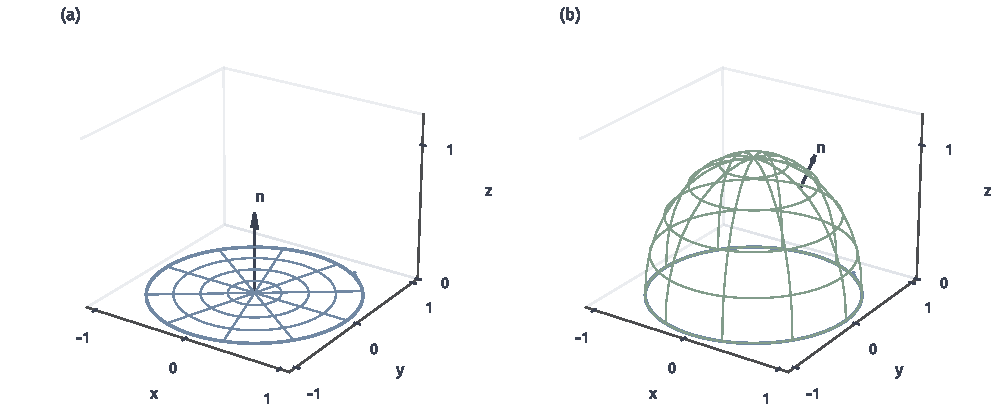
\includegraphics[width=169.0mm]{figures/00-shared/mathematical-preliminaries-upper/00-shared/matplotlib/chapter3-concept-processes/stokes-spanning-surfaces.pdf}
 \caption{(a) 向上单位圆盘；(b) 外向上半单位球面。蓝色边界均从上方看逆时针，黑箭头标记各自法向。对$F=(-y/2,x/2,0)^\top$，旋度恒为$(0,0,1)^\top$，两面上的旋度通量都为$\pi$。右面面积为$2\pi$而非$\pi$；相等的是法向分量的累计，不能把通量当成面积。}
 \label{fig:analysis-process-stokes-spanning-surfaces}
\end{figure*}

\subsection{积分分部与Green恒等式}

积分分部把导数从一个因子转移到另一个因子，同时保留边界上的贡献。

设$\Omega$满足Gauss公式的区域条件，标量函数$u$与向量场$\bm F$在$\overline\Omega$的开邻域内都是$C^1$。逐坐标使用乘积法则，得
\[
 \operatorname{div}(u\bm F)=\nabla u^\top\bm F+u\operatorname{div}\bm F.
\]
对两边积分并使用Gauss公式，移项得到
\[
 \int_\Omega u\operatorname{div}\bm F\,\mathrm dV
 =\int_{\partial\Omega}u\bm F^\top\bm n\,\mathrm dS
 -\int_\Omega\nabla u^\top\bm F\,\mathrm dV.
\]
若边界上$u=0$，或$\bm F$的法向分量为零，边界项消失；一般情况下必须保留它。取$\bm F=\nabla v$便联系到二阶微分，下面将这一情形写成正式结论。

一元分部积分（式~\eqref{eq:analysis-integration-by-parts}）把一个因子的导数转给另一个因子，并留下端点项。

设$u$在$[a,b]$上连续可微、$v$二阶连续可微，把式中的$v$换成$v'$，得到
\[
 \int_a^bu\,v''\,\mathrm dx
 =u(b)v'(b)\cdot(+1)+u(a)v'(a)\cdot(-1)-\int_a^bu'v'\,\mathrm dx.
\]
这里把端点项$[uv']_a^b$拆开写：区间在右端点的外法向是$+1$，在左端点是$-1$。

推广到多元情形时，各项依次对应：二阶导数$v''$换成$\Delta v$，一阶导数的乘积$u'v'$换成梯度的内积$\nabla u^\top\nabla v$，两个端点换成边界曲面，“$v'$乘外法向$\pm1$”换成$\nabla v^\top\bm n$，即$v$沿外法向的方向导数。
对乘积向量场$u\nabla v$使用散度定理，就得到这一推广。
\begin{theorem}[多元分部积分]
\label{thm:multivariable-integration-by-parts}
设$\Omega\subseteq\mathbb R^3$满足上述Gauss公式的区域条件。
若标量函数$u$在$\overline\Omega$的开邻域内连续可微，$v$在同一邻域内二阶连续可微，则
\[
 \int_\Omega u\Delta v\,\mathrm d\bm x
 =\int_{\partial\Omega}u\nabla v^\top\bm n\,\mathrm dS
  -\int_\Omega\nabla u^\top\nabla v\,\mathrm d\bm x.
\]
\end{theorem}
\begin{proof}
向量场$\bm F=u\nabla v$的第$j$个分量是$u\,\partial_jv$，它连续可微。由一元乘积法则，
$\partial_j(u\,\partial_jv)=\partial_ju\,\partial_jv+u\,\partial_j^2v$，对$j$求和得到
\[
 \operatorname{div}(u\nabla v)
 =\nabla u^\top\nabla v+u\Delta v.
\]
将它代入Gauss公式，再把$\nabla u^\top\nabla v$的区域积分移到等式另一侧，即得结论。
\end{proof}
对满足Green公式条件的平面区域，同样的证明改用平面通量公式（定理~\ref{thm:multivariable-planar-flux}）即可，边界面积元素相应换成弧长元素。
这一公式把$v$的二阶导数转移为$u$与$v$的一阶导数，同时保留法向边界项；该项是否为零，必须由具体边界条件决定。

取$u=1$，公式化为$\int_\Omega\Delta v\,\mathrm d\bm x=\int_{\partial\Omega}\nabla v^\top\bm n\,\mathrm dS$，也就是对梯度场$\nabla v$使用散度定理。下面在球上核对这一特例。
\begin{example}[球上平方范数的Laplace积分]
取以原点为中心、半径为$R$的球$B_R$和$v(\bm x)=\lVert\bm x\rVert_2^2$。
左侧：$\Delta v=6$，所以$\int_{B_R}\Delta v\,\mathrm d\bm x=6\operatorname{vol}(B_R)=6\cdot\frac{4\pi R^3}3=8\pi R^3$。
右侧：球面上$\nabla v=2\bm x$，外法向$\bm n=\bm x/R$，故$\nabla v^\top\bm n=2\lVert\bm x\rVert_2^2/R=2R$，积分为$2R\cdot4\pi R^2=8\pi R^3$。两侧相等。
\end{example}

边界项为零时，公式可以给出结构性的结论。下面用它说明Laplace方程的解由边界值唯一确定。
\begin{example}[Laplace方程的解由边界值决定]
设$\Omega$满足Gauss公式的区域条件，$w$在$\overline\Omega$的开邻域内二阶连续可微，在$\Omega$内$\Delta w=0$，在$\partial\Omega$上$w=0$。
在定理~\ref{thm:multivariable-integration-by-parts}中取$u=v=w$。左侧被积函数$w\Delta w$为零；边界项的被积函数含因子$w$，也为零。于是
\[
 \int_\Omega\lVert\nabla w\rVert_2^2\,\mathrm d\bm x=0.
\]
被积函数连续且非负；若它在某点为正，则在该点的一个邻域内为正，积分也为正。所以在开集$\Omega$上$\nabla w$恒为零。
$\Omega$是连通的开区域，所以$w$在$\Omega$上为常数；再由$w$在$\overline\Omega$上连续且在边界上为零，得$w\equiv0$。

现在设$v_1,v_2$都在$\overline\Omega$的开邻域内二阶连续可微，在$\Omega$内满足$\Delta v_1=\Delta v_2=0$，在$\partial\Omega$上取值相同。差$w=v_1-v_2$满足上面的全部条件，所以$v_1=v_2$。
\end{example}
按热传导的解释，稳定的温度分布由边界温度唯一决定。

若$u,v$都为$C^2$函数，交换分部积分公式中的$u,v$，再将两式相减，梯度内积项抵消，得到Green第二恒等式：
\[
 \int_\Omega (u\Delta v-v\Delta u)\,\mathrm d\bm x
 =\int_{\partial\Omega}(u\nabla v-v\nabla u)^\top\bm n\,\mathrm dS.
\]
前面的分部积分公式也称Green第一恒等式。两式都要求同样的区域规则性和边界定向；第二式通过交换两个函数，显示边界项怎样控制Laplace作用在积分配对中的交换。

\paragraph{积分公式的比较}

本节各公式回答的都是同一类问题：导数在内部的积分与边界积分之间的关系。推导方式也相同：在小块上建立局部关系，再利用相容方向让内部边界相消。
它们的内部对象、边界对象和方向条件则各不相同。下表把一元基本定理与路径积分基本定理也列在一起，二者以区间或路径的两个端点为边界。
\begin{center}
\begin{tabular}{lll}
\toprule
公式 & 内部积分 & 边界积分\\
\midrule
一元基本定理 & 区间上的$f'$ & 端点值之差$f(b)-f(a)$\\
路径积分基本定理 & 路径上$\nabla\phi$的切向积分 & 端点值之差\\
Green环流形式 & 平面区域的$Q_x-P_y$ & 正向路径的切向积分\\
Gauss & 空间区域的散度 & 闭曲面的外向通量\\
Stokes & 定向曲面的旋度通量 & 诱导方向的路径环流\\
\bottomrule
\end{tabular}
\end{center}
对向上定向的平面曲面，Stokes公式还原为Green公式的环流形式；Green公式的通量形式则是二维的散度公式。
普通标量函数的区域积分不自动具有边界表达：要使用这些公式，须先找到满足条件的向量场，使其散度或旋度的相应分量等于被积函数。示例~\ref{ex:analysis-green-area-formula}的面积公式就是先选出满足$Q_x-P_y\equiv1$的场。

Stokes公式还解释了第~\ref{sec:multivariable-potential-path-independence}节中势函数的存在为何与定义域有关。设$\bm F$在开集$U\subseteq\mathbb R^3$上连续可微且$\nabla\times\bm F=\bm0$。若一条闭路径是$U$内某张满足定理条件的定向曲面的有向边界，则该闭路径上的环流等于旋度的通量，也就是零。
在星形域中，闭路径上各点与中心点之间的线段扫出一张锥面，它整个落在定义域内，不会碰到场的奇点；这与那里在星形域上构造势函数的结论一致。
穿孔平面上绕原点的单位圆则不同：在平面内，以它为边界的区域只能是单位圆盘，必然包含原点，而场在原点无定义；所以局部条件$Q_x-P_y=0$并不排除$2\pi$的环流（示例~\ref{ex:analysis-annulus-vortex-green}）。

各公式均使用本章的经典积分。连续可微性、分片规则边界与定向是这里的经典公式所需的条件，并不是另换一种积分定义。
尤其要核对向量场是否在整个积分对象附近都有定义：穿孔平面上的涡旋场在原点无定义，不能把包含原点的圆盘直接代入Green公式；点源场也不能直接用于包含原点的球体（示例~\ref{ex:analysis-point-source-flux}）。
区域积分中可以忽略的边界，对边界积分却正是累计对象。因此必须指定场在边界处的实际取值，并检查其连续可微的延拓，不能只凭区域内部的积分值推断边界积分。
如果要降低导数或边界的规则性，还须另外建立弱导数、边界迹及相应的积分公式；不能沿用当前公式而省去这些条件。

\FloatBarrier


\FloatBarrier
\section{本章小结}
\label{sec:multivariable-summary}

区域积分把密度累计成总量；连续性和规则的区域边界保证可以逐个坐标切片计算，Jacobian行列式的绝对值给出坐标变换下的体积缩放。第一类路径积分与曲面积分按弧长和面积累计，不依赖方向；第二类路径积分计算做功，第二类曲面积分计算通量，二者都随方向反转而变号。

保守场的功只取决于端点。交叉偏导相等在星形区域上保证势函数存在，在有孔的区域上则不够。散度是单位体积的净流出，旋度是单位面积的环流；Green、Gauss和Stokes公式将内部的散度或旋度累计与边界上的通量或环流联系起来。使用这些公式时，应检查域内奇点、场的光滑性、完整边界及其定向。
